% !TeX root = main.tex
% !TeX spellcheck = fr_FR
\documentclass[12pt,a4paper,twoside]{article}
\usepackage[scaled]{helvet}
% Packages and macros
\usepackage[T1]{fontenc}

\usepackage{graphicx}

\usepackage{mathptmx}
\usepackage{pgf}
\usepackage{pgfpages}
\usepackage{booktabs}
\usepackage{fancyhdr}
\usepackage{datetime}
\usepackage{enumerate}
\usepackage{pifont}
\usepackage{amssymb}
\usepackage[export]{adjustbox}
\usepackage[margin=1in]{geometry}
\usepackage[french]{babel}
\usepackage{caption}
\usepackage{tikz}
\usepackage{tabularx}
\usepackage{gensymb}
\usepackage{pdfpages}
\usepackage{caption}
\usepackage{subcaption}
\usepackage{listings}
\usepackage{afterpage}

\usepackage[bottom]{footmisc}

\usepackage{textcomp}


\usepackage{fontawesome5}

\usepackage{hyperref}
\hypersetup{
	colorlinks=true,
	linkcolor=blue,
	filecolor=magenta,      
	urlcolor=cyan,
	pdftitle={Overleaf Example},
	pdfpagemode=FullScreen,
}

\usepackage[sort=none, abbreviations]{glossaries-extra}

\newglossaryentry{centrale inertielle}
{
	name=Centrale inertielle,
	description={Instrument utilisé en navigation, capable d'intégrer les mouvements d'un mobile (accélération et vitesse angulaire) pour estimer son orientation (angles de roulis, de tangage et de cap), sa vitesse linéaire et sa position.}
}
\newglossaryentry{timestamp}
{
	name=Timestamp,
	description={Enrengistrement de l'heure et/ou la date d'un événement.}
}

\newglossaryentry{GPS}
{
	name=GPS,
	description={Le système de positionnement global (GPS) est un service public américain qui fournit aux utilisateurs des services de positionnement, de navigation et de synchronisation (PNT). Ce système se compose de trois segments : le segment spatial, le segment de contrôle et le segment utilisateur. L'U.S. Space Force développe, entretient et exploite les segments spatial et de contrôle.}
}

\newglossaryentry{GNSS}
{
	name=GNSS,
	description={Le système mondial de navigation par satellite (GNSS) est un terme général décrivant toute constellation de satellites qui fournit des services de positionnement, de navigation et de synchronisation (PNT) à l'échelle mondiale ou régionale.}
}

\newglossaryentry{PIC32}
{
	name=PIC32,
	description={Famille de microcontrôleur 32-bits de Microchip.}
}
\newglossaryentry{FTDI}
{
	name=FTDI,
	description={Composant Future Technology Devices International. Ici sert de convertisseur USB to UART.}
}
\newglossaryentry{harmony}
{
	name=Harmony,
	description={Configurateur graphique / générateur de code pour les microcontrôleurs de Microchip.}
}

\newglossaryentry{datasheet}
{
	name=Datasheet,
	description={Document du fabricant fournissant les spécifications d'un produit.}
}


\newabbreviation{mcu}{MCU}{microcontrôleur.}
\newabbreviation{pcb}{PCB}{circuit imprimé.}
\newabbreviation{imu}{IMU}{centrale inertielle.}
\newabbreviation{rf}{RF}{radio-fréquence.}
\newabbreviation{gps}{GPS}{global Positioning System.}
\newabbreviation{gnss}{GNSS}{global navigation satellite systems.}





\newcommand{\source}[1]{\vspace{-11pt} \caption*{\small \textit{Source: {#1}} }}

\newcommand\blankpage{%
	\null
	\thispagestyle{empty}%
	\addtocounter{page}{-1}%
	\newpage}

\usepackage{verbatim}

\newdateformat{monthyeardate}{%
  \monthname[\THEMONTH], \THEYEAR}

\begin{document}
\pagestyle{fancy}
\lhead{Travail de diplôme 1924B}
\chead {\today}
\rhead{Mini boîte noire}

% ------------------------- TITLE PAGE INSERTION ------------------------
\begin{titlepage} % Suppresses displaying the page number on the title page and the subsequent page counts as page 1
	\newcommand{\HRule}{\rule{\linewidth}{0.5mm}} % Defines a new command for horizontal lines, change thickness here
	
	\center % Centre everything on the page
	
	%------------------------------------------------
	%	Headings
	%------------------------------------------------
	
	\textsc{\LARGE Ecole des métiers de Lausanne \\ Ecole supérieure}\\[1.5cm] % Main heading such as the name of your university/college
	
	\textsc{\Large Génie électrique}\\[0.5cm] % Major heading such as course name
	
	\textsc{\large Système d'enregistrement de trajectoires de vol}\\[0.5cm] % Minor heading such as course title
	
	%------------------------------------------------
	%	Title
	%------------------------------------------------
	
	\HRule\\[0.4cm]
	
	{\huge\bfseries Boîte noire miniaturisée}\\[0.4cm] % Title of your document
	
	\HRule\\[1.5cm]
	
	%------------------------------------------------
	%	Author(s)
	%------------------------------------------------
	
	\begin{minipage}{0.4\textwidth}
		\begin{flushleft}
			\large
			\textit{Auteur}\\
			Ali \textsc{Zoubir} % Your name
		\end{flushleft}
	\end{minipage}
	~
	\begin{minipage}{0.4\textwidth}
		\begin{flushright}
			\large
			\textit{Superviseur}\\
			Juan José \textsc{Moreno} % Supervisor's name
		\end{flushright}
	\end{minipage}
	
	% If you don't want a supervisor, uncomment the two lines below and comment the code above
	%{\large\textit{Author}}\\
	%John \textsc{Smith} % Your name
	
	%------------------------------------------------
	%	Date
	%------------------------------------------------
	
	\vfill
	\vfill
	%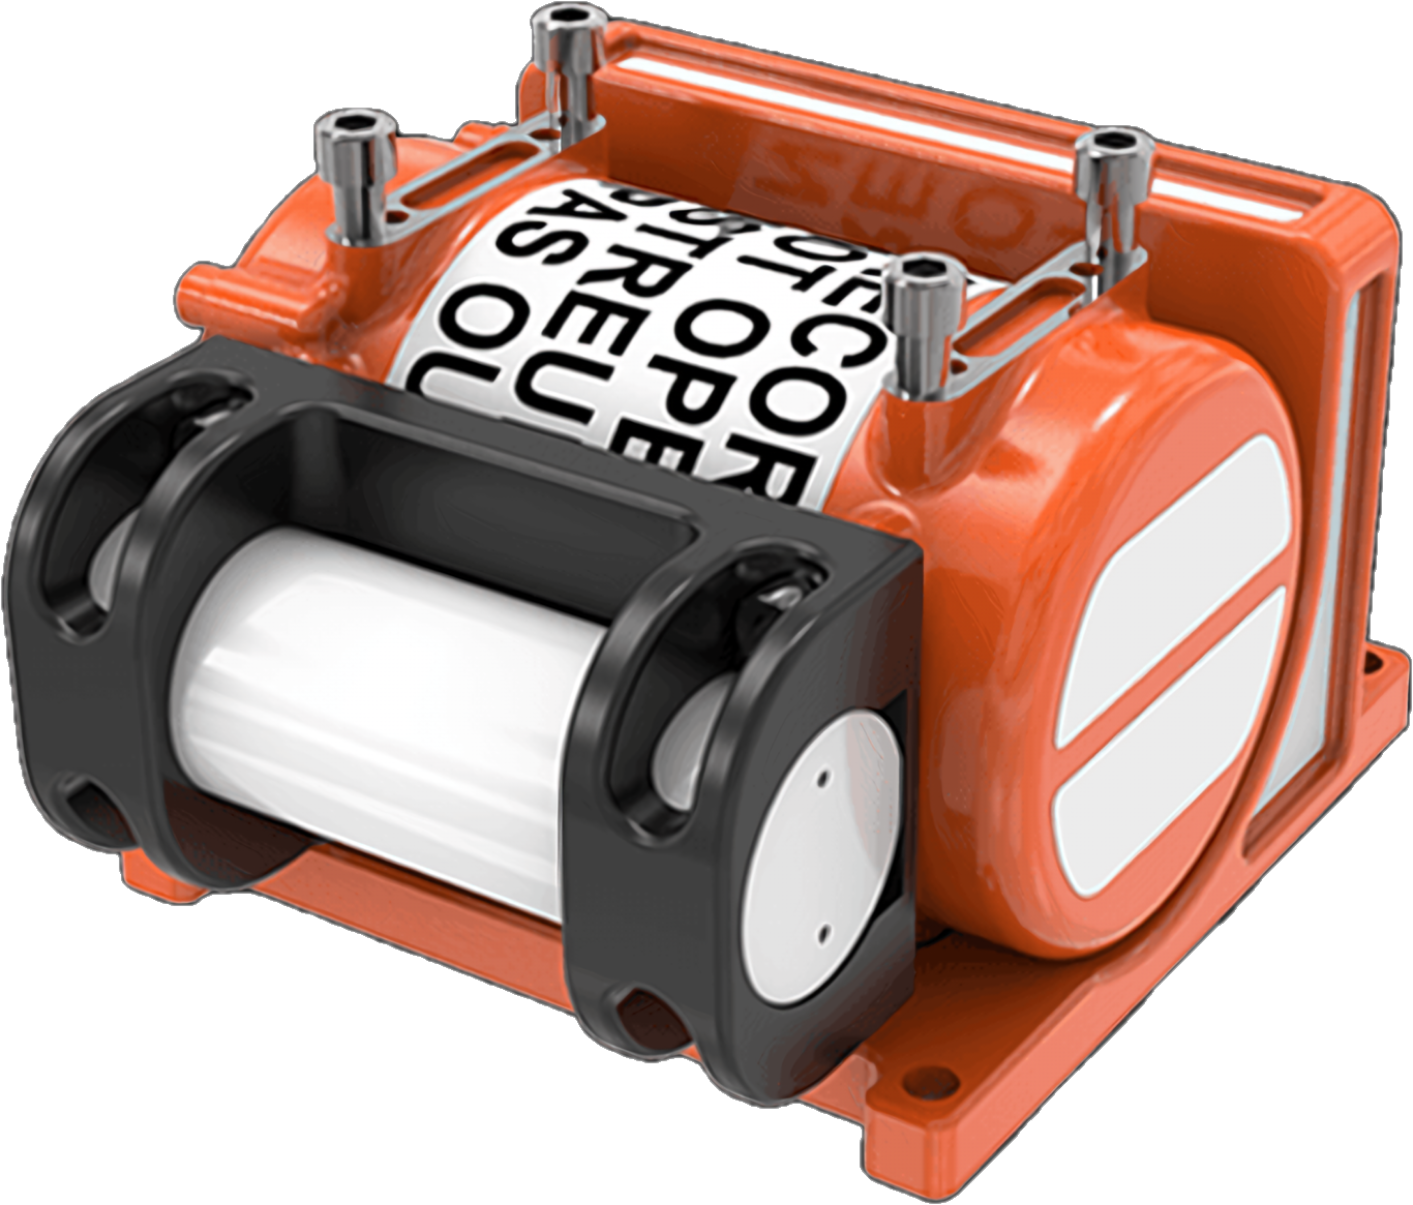
\includegraphics[width=5cm]{LOGO-PROJ}
	% \vfill\vfill\vfill % Position the date 3/4 down the remaining page
	\vfill
	
	{\large\today} % Date, change the \today to a set date if you want to be precise
	
	%------------------------------------------------
	%	Logo
	%------------------------------------------------
	
	%\vfill\vfill
	%\includegraphics[width=0.2\textwidth]{placeholder.jpg}\\[1cm] % Include a department/university logo - this will require the graphicx package
	
	%----------------------------------------------------------------------------------------
	
	\vfill % Push the date up 1/4 of the remaining page
	
\end{titlepage} 
\afterpage{\blankpage}

\clearpage

% --------------------- TABLE OF CONTENTS  ------------------------------- 
\tableofcontents
\clearpage

\printunsrtglossary[type=abbreviations]
\printunsrtglossary % default: style=list, type=main

% ---------- CAHIER DES CHARGES ---------------------------------\\
\onecolumn

\begin{figure}
	\begin{minipage}{0.47\textwidth}
		\centering
		
\includegraphics[width=.4\textwidth,left,]{./ETML-ES-LOGO.png}
	\end{minipage}
	
	\hfill
	\begin{minipage}{0.7\textwidth}
		\raggedleft
		\LARGE \textbf{Boîte noire miniaturisée\\ 2023, 1942B}
	\end{minipage}
\end{figure}


% ---- DESCRIPTION ----
\section{Cahier des charges}
\noindent
\begin{minipage}[t]{.5\textwidth} %
	\subsection{Introduction}
	Ce projet vise à stocker les données de mesures et de localisation d'un avion en utilisant une centrale inertielle et un GPS/GNSS. En combinant ces technologies, nous pouvons enregistrer des informations précises sur les caractéristiques du vol et la trajectoire de l'avion. En cas d'accident, ces enregistrements permettent de déterminer les causes potentielles. En somme, ce système de collecte et de stockage de données fournit une compréhension approfondie des vols et des données essentielles. Le cahier des charges détaillé est disponible en annexe.
\end{minipage} %
\begin{minipage}[t]{.5\textwidth} %
	\raggedleft
	\subsection{Aperçu}
	\begin{itemize}
		\item[•]	Sauvegarde des données inertielles chaque 500ms par défaut.
		\item[•]	Sauvegarde des données de localisation chaque 5'000ms par défaut.
		\item[•]	Possibilité de configurer les temps de sauvegarde.
		\item[•]	Résistance aux chocs.
		\item[•]	Bonne autonomie / Low power.
		\item[•]	\Gls{gps}
		\item[•]	\Gls{gnss}.
		\item[•]	\Gls{timestamp} par satellite.
		\item[•]	\gls{centrale inertielle} :
		\subitem- 	Accéléromètre 3-axes. 
		\subitem-	Gyroscope 3-axes.
		\item[•] Charge, lecture et config. par USB-C.
	\end{itemize}
\end{minipage}

% ---- TACHES ----
\subsection{Tâches à réaliser}
Développement et intégration d’un PCB avec capteurs et logging sur carte SD dans un boitier compact.
\begin{itemize}
	\item[•] Développement schématique 
	\subitem- Fonctionnement MCU.
	\subitem-	Périphériques de mesures et de sauvegarde / Bus de communication.
	\subitem-	Gestion batterie 
	\item[•]	Routage pour intégration dans boitier résistant aux chocs.
	\item[•]	Programmation mesure et sauvegarde des données.
	\subitem-	Configuration MCU.
	\subitem-	Configuration du périphérique de mesure pour \gls{imu}.
	\subitem-	Configuration du périphérique de sauvegarde (Carte SD).
	\subitem-	Configuration du périphérique de localisation \gls{gps}/\gls{gnss}.
	\subitem-	Configuration et communication avec l'interface.
	\subitem-	Communication et traitement des données mesurées.
\end{itemize}

\subsection{Schéma de principe}
% ---- SChema de principe ----
\begin{figure}[h]
	\centering
	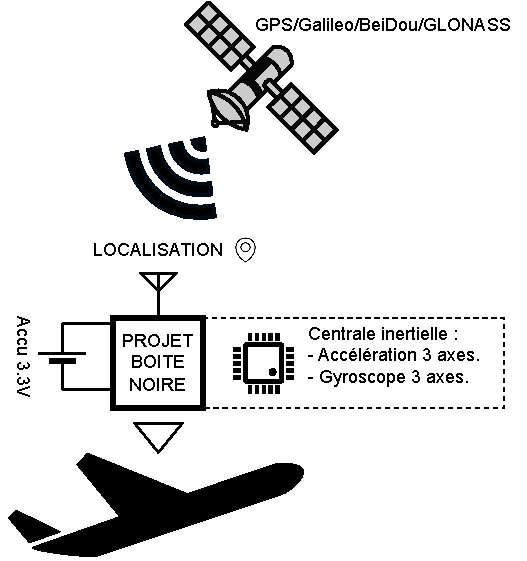
\includegraphics[width=0.6\linewidth]{../figures/cdc/schema_principe}
	\caption{Schéma de principe.}
	\source{Auteur}
	\label{fig:schemaprincipe}
\end{figure}

Ce système électronique de mini boîte noire pour avion, serait capable d'enregistrer des informations récentes sur les données inertielle et la position d'un vol, dans une mémoire non volatile (carte microSD). Le dispositif, abrité dans un boîtier plastique pour assurer une réception optimale des données GPS et une installation compact. Celui-ci fournirait des données via un port USB pour l'extraction des mesures sur la carte microSD ou pour configurer des paramètres tels que les intervalles de mesures. Les mesures sur les trois axes d'accélération et de vitesse angulaire seraient recueillies par défaut toutes les 500 ms et les données de position GPS toutes les 5000 ms. Des intervalles d'enregistrement plus longs sont envisageables pour optimiser la durée de vie de la carte SD, selon la taille et l'organisation des données. Le dispositif sauvegarderait les données des 15 dernières minutes de vol (ou plus) dans un fichier CSV pour traitement ultérieur, selon le principe FIFO. L'objectif principal du prototype est de privilégier la compacité pour minimiser son encombrement à bord de l'avion.


\clearpage

% ---- JALONS ----
\subsection{Planification}
\begin{figure}[h]
	\centering
	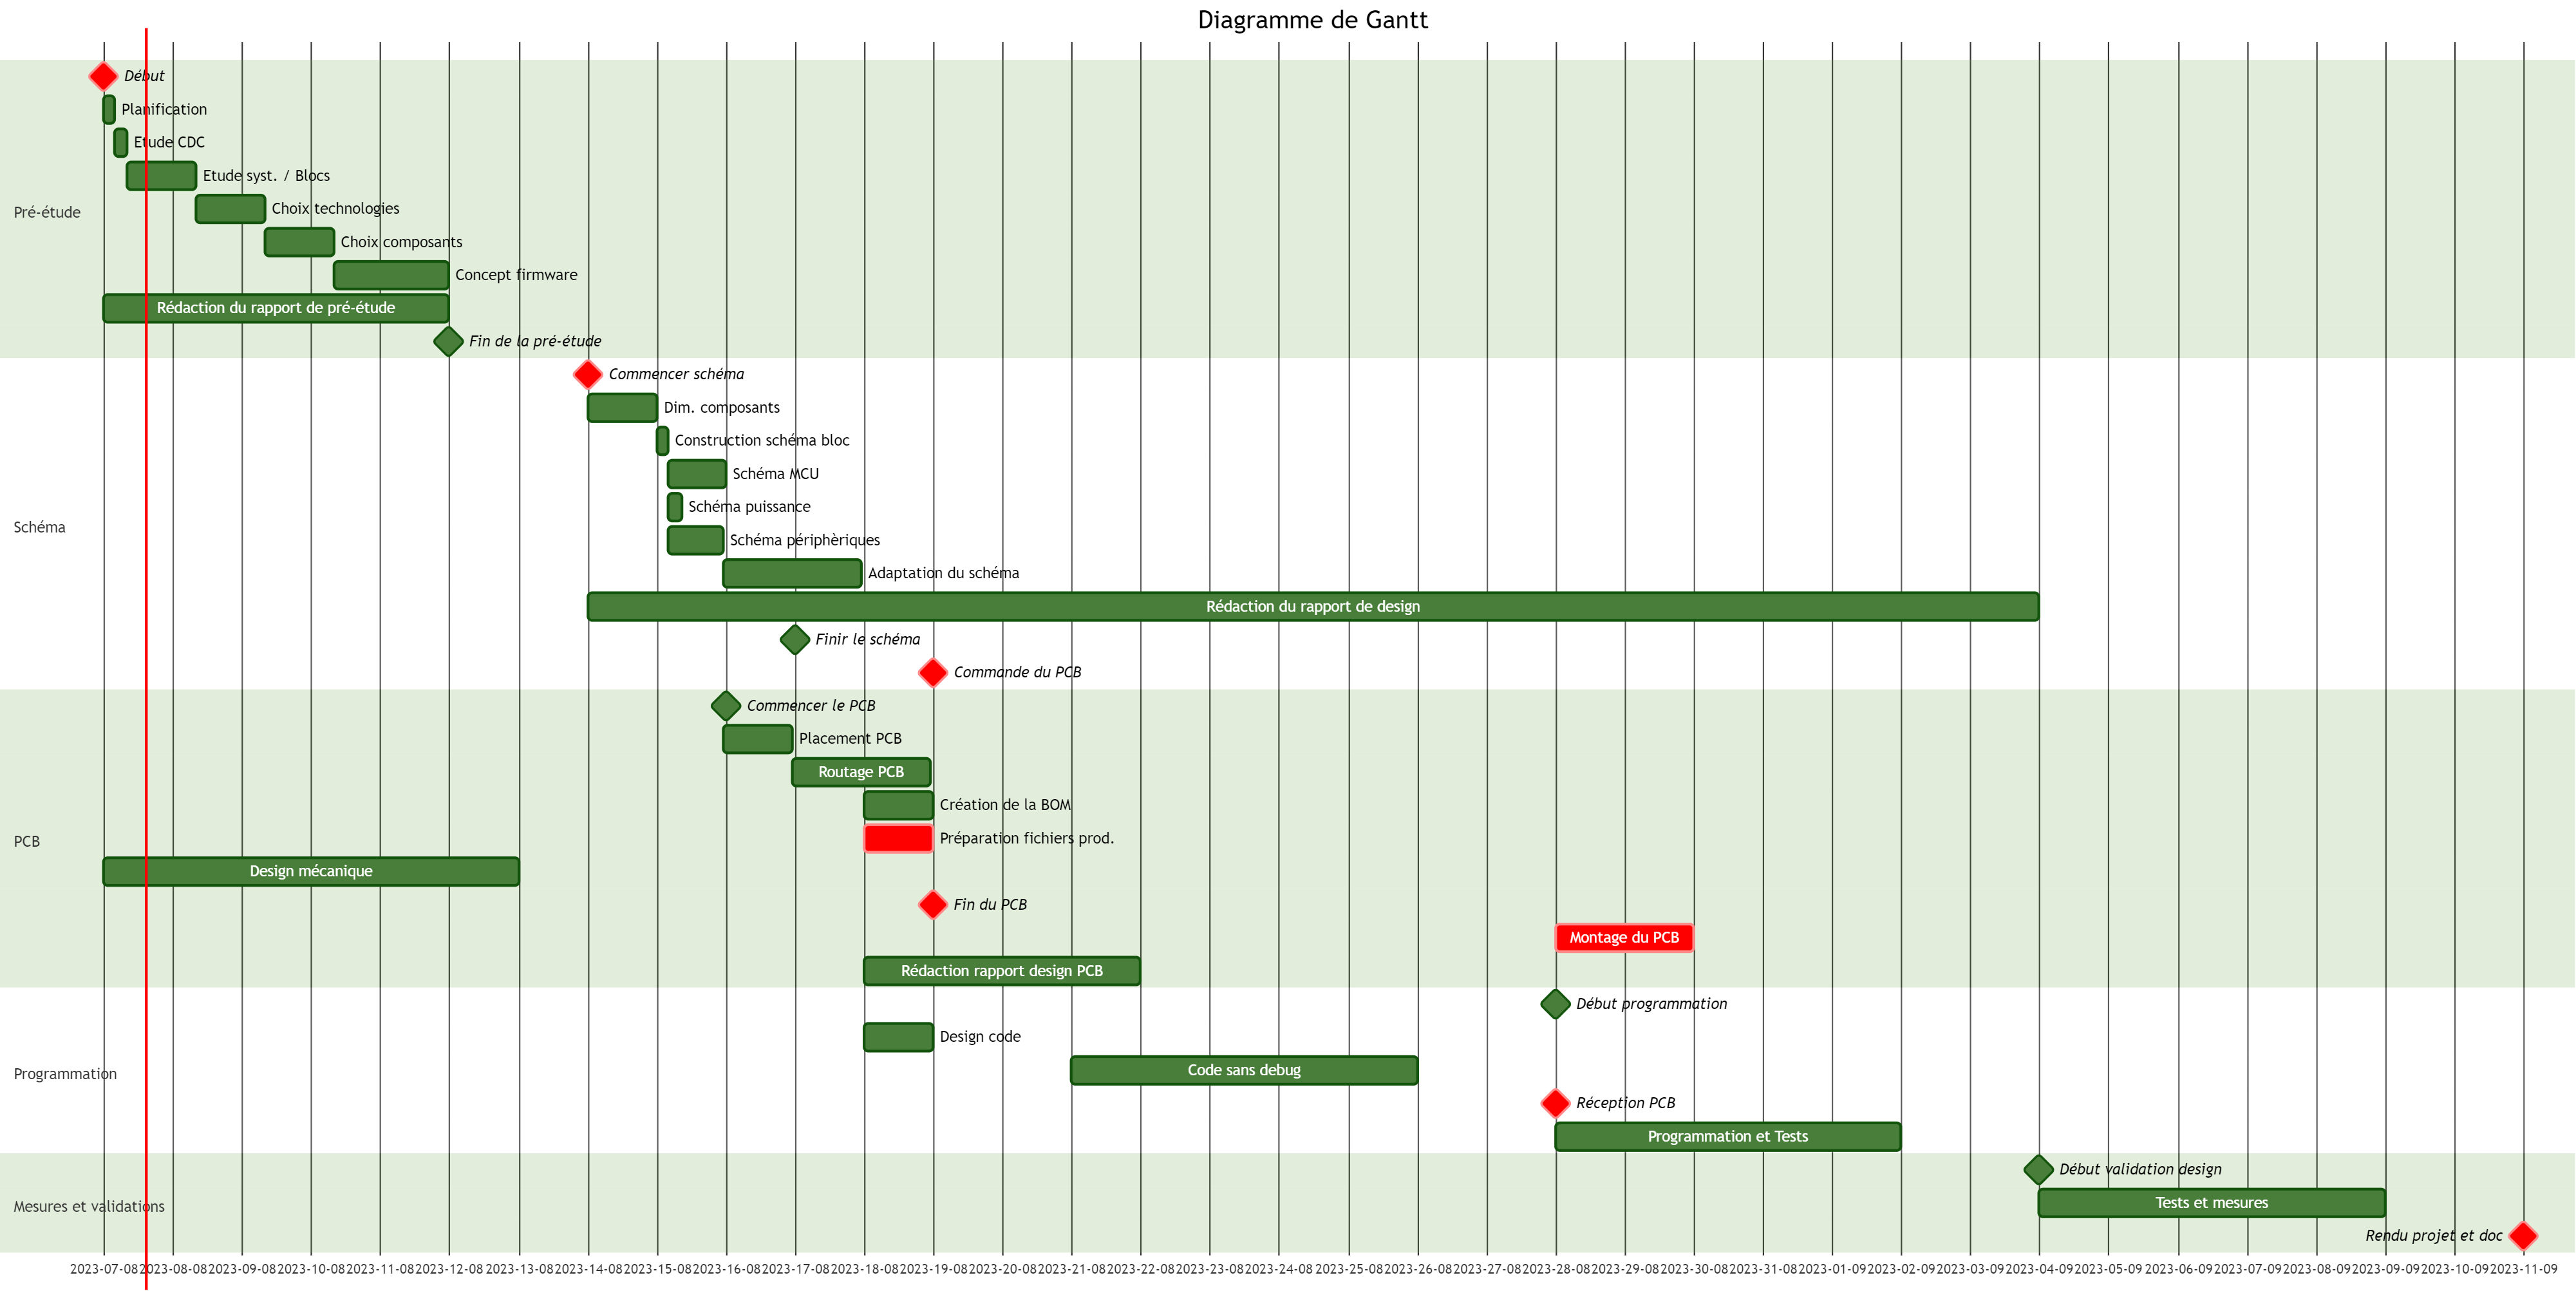
\includegraphics[width=1\linewidth]{../figures/cdc/planif}
	\caption{Planification, Diagramme de gantt.}
	\source{Auteur}
	\label{fig:planification}
\end{figure}
\begin{figure}[h]
	\centering
	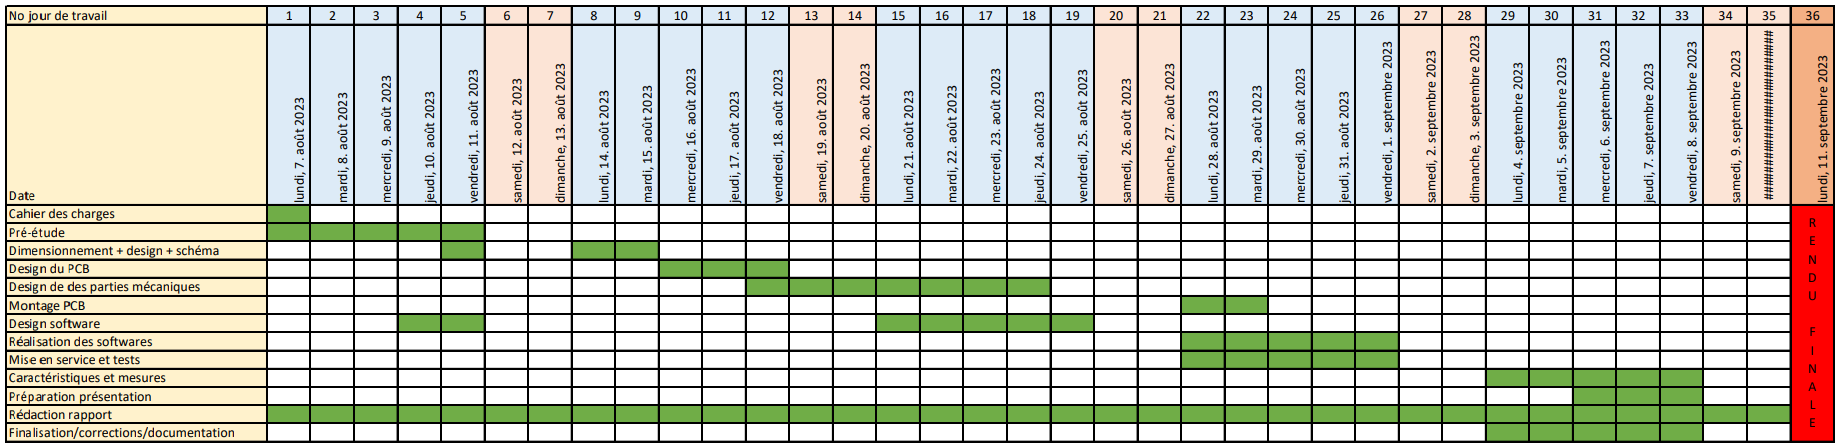
\includegraphics[width=1\linewidth]{../figures/cdc/planif_theorique}
	\caption{Planification théorique.}
	\source{Auteur}
	\label{fig:planiftheorique}
\end{figure}


\subsection{Livrable}
\begin{itemize}
	\item[•] Les fichiers sources de CAO électronique des PCB réalisés
	\item[•] Tout le nécessaire à fabriquer un exemplaire hardware de chaque :
	\item[•] fichiers de fabrication (GERBER) / liste de pièces avec références pour commande / implantation
	\item[•] Prototype fonctionnel
	\item[•] Modifications / dessins mécaniques, etc
	\item[•] Les fichiers sources de programmation microcontrôleur (.c  / .h)
	\item[•] Tout le nécessaire pour programmer les microcontrôleurs (logiciel ou fichier .hex)
	\item[•] Un calcul / estimation des coûts
	\item[•] Un rapport contenant les calculs - dimensionnement de composants - structogramme, etc.
\end{itemize}

\clearpage


% ------------------- PRE-ETUDE ---------------------------------
\section{Pré-étude} \label{sec:Pre-Etude}

\subsection{Choix des composants importants} \label{ssec:Choix-composant}

\subsubsection{Centrale inertielle} \label{sssec:Choix-Centrale-inertielle}

\subsubsection{GPS / GNSS} \label{sssec:Choix-GPS}

\subsubsection{Microcontrôleur} \label{sssec:Choix-MCU}

\subsubsection{Batterie, charge et régulation} \label{sssec:Choix-Batterie-charge}

\subsection{Estimation des coûts} \label{sssec:Estimation-Couts}


% ---------- DÉVELOPPEMENT SCHÉMATIQUE --------------------------
\section{Développement du schéma électronique} \label{sec:Dev-Schematique}
Dans cette section, nous décrirons la phase principale du développement ainsi que la démarche suivie pour élaborer le schéma électronique du projet.

\subsection{Blocs développés} \label{ssec:Dev-blocs}
Pour faciliter le développement et la lecture du schéma, il est judicieux de diviser le système en plusieurs blocs. Une structure a ainsi été définie, divisant le circuit en trois blocs principaux : \hyperref[ssec:Dev-MCU]{\textbf{Microcontrôleur \ref{ssec:Dev-MCU}}} (Intelligence du système, connexion du programmeur et LED de vie.), \hyperref[ssec:Dev-Devices]{\textbf{Périphériques \ref{ssec:Dev-Devices}}} (\gls{GNSS}, \gls{imu}, \gls{FTDI}, connecteur USB, Carte SD.) et \hyperref[ssec:Dev-Alim]{\textbf{Alimentations \ref{ssec:Dev-Alim}}} (Connecteur batterie, gestion de charge, régulateurs de tension et système ON/OFF.).

Nous pouvons sur la figure \ref{fig:blocs} observer les différentes interaction entre les blocs, elles sont par la suite décrites dans le tableau \ref{tab:descrConnexion}.

\begin{figure}[h]
	\centering
	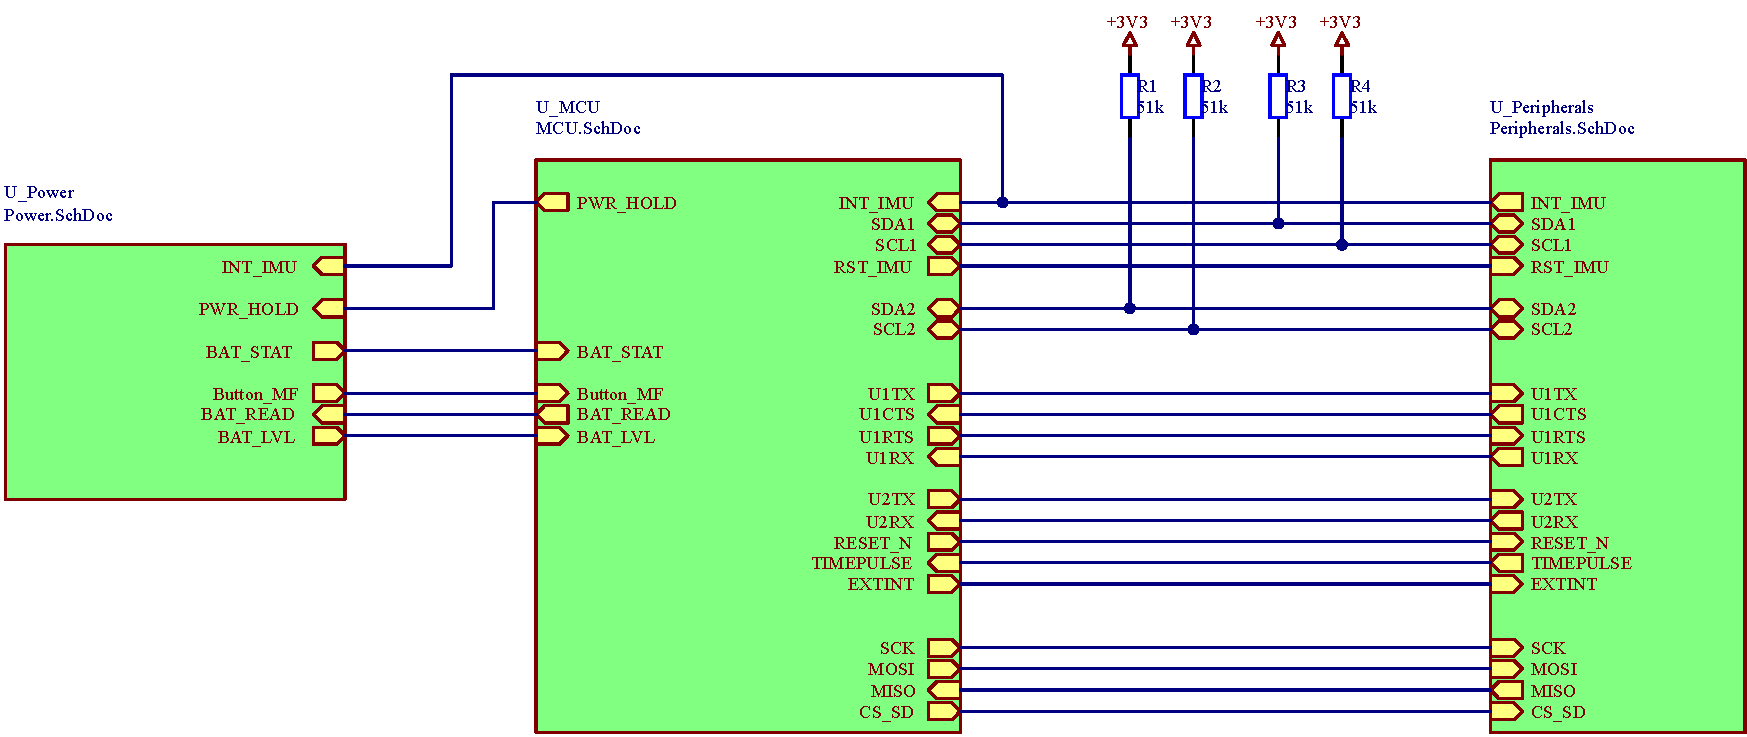
\includegraphics[width=.85\linewidth]{../figures/etude/sch/BLOCS}
	\caption{Blocs du système.}
	\source{Auteur}
	\label{fig:blocs}
\end{figure}

\begin{table}[h]
		\centering
		\resizebox{\columnwidth}{!}{%
			\begin{tabular}{l|l}
				Connexion/s & Description \\
				\hline
				INT\_IMU & Interruption de la centrale inertielle, informe le \gls{mcu} et peut allumer le système. \\ 
				RST\_IMU & Permet de réinitialiser la \gls{imu}. \\
				PWR\_HOLD & Le \gls{mcu} peut se maintenir alimenté par cette connexion. \\
				BAT\_STAT & Fournit le statut de la batterie au \gls{mcu}. \\
				Button\_MF & Fournit le niveau logique du bouton au \gls{mcu}. \\
				BAT\_READ & Le \gls{mcu} peut activer la lecture de la tension de la batterie. \\
				BAT\_LVL & Lecture analogique de la tension de batterie. \\
				SDA1, SCL1 & Communication I2C avec l'\gls{imu}. \\
				SDA2, SCL2 & Communication I2C optionnelle avec le \gls{GNSS}. \\
				U1TX/RX... & Communication UART avec le \gls{FTDI} pour l'USB. \\
				U2TX/RX & Communication UART avec le \gls{GNSS}. \\
				RESET\_N & Permet de réinitialiser le \gls{GNSS}. \\
				TIMEPULSE & Permet de mesurer le temps par un signal pulsé. \\
				EXTINT & Permet de gérer le mode d'alimentation du \gls{GNSS} \\
				SCK, MOSI... & Communication SPI avec la carte SD. \\ 
				R1,2,3,4 & Résistances de PULL-UP pour communication I2C. \\
			\end{tabular}
		}
		\caption{Description des connexions}
		\label{tab:descrConnexion}
	\end{table}

\clearpage

\subsection{Microcontrôleur} \label{ssec:Dev-MCU}

\subsubsection{Connexion} 
Pour utiliser le microcontrôleur, il est nécessaire de définir ses entrées/sorties en se référant à son \gls{datasheet}. Ce dernier permet de connaître les connexions dédiées à certains bus de communication ou à des entrées analogiques. 

\begin{figure}[h]
	\centering
	\begin{subfigure}[b]{0.6\textwidth}
		\centering
		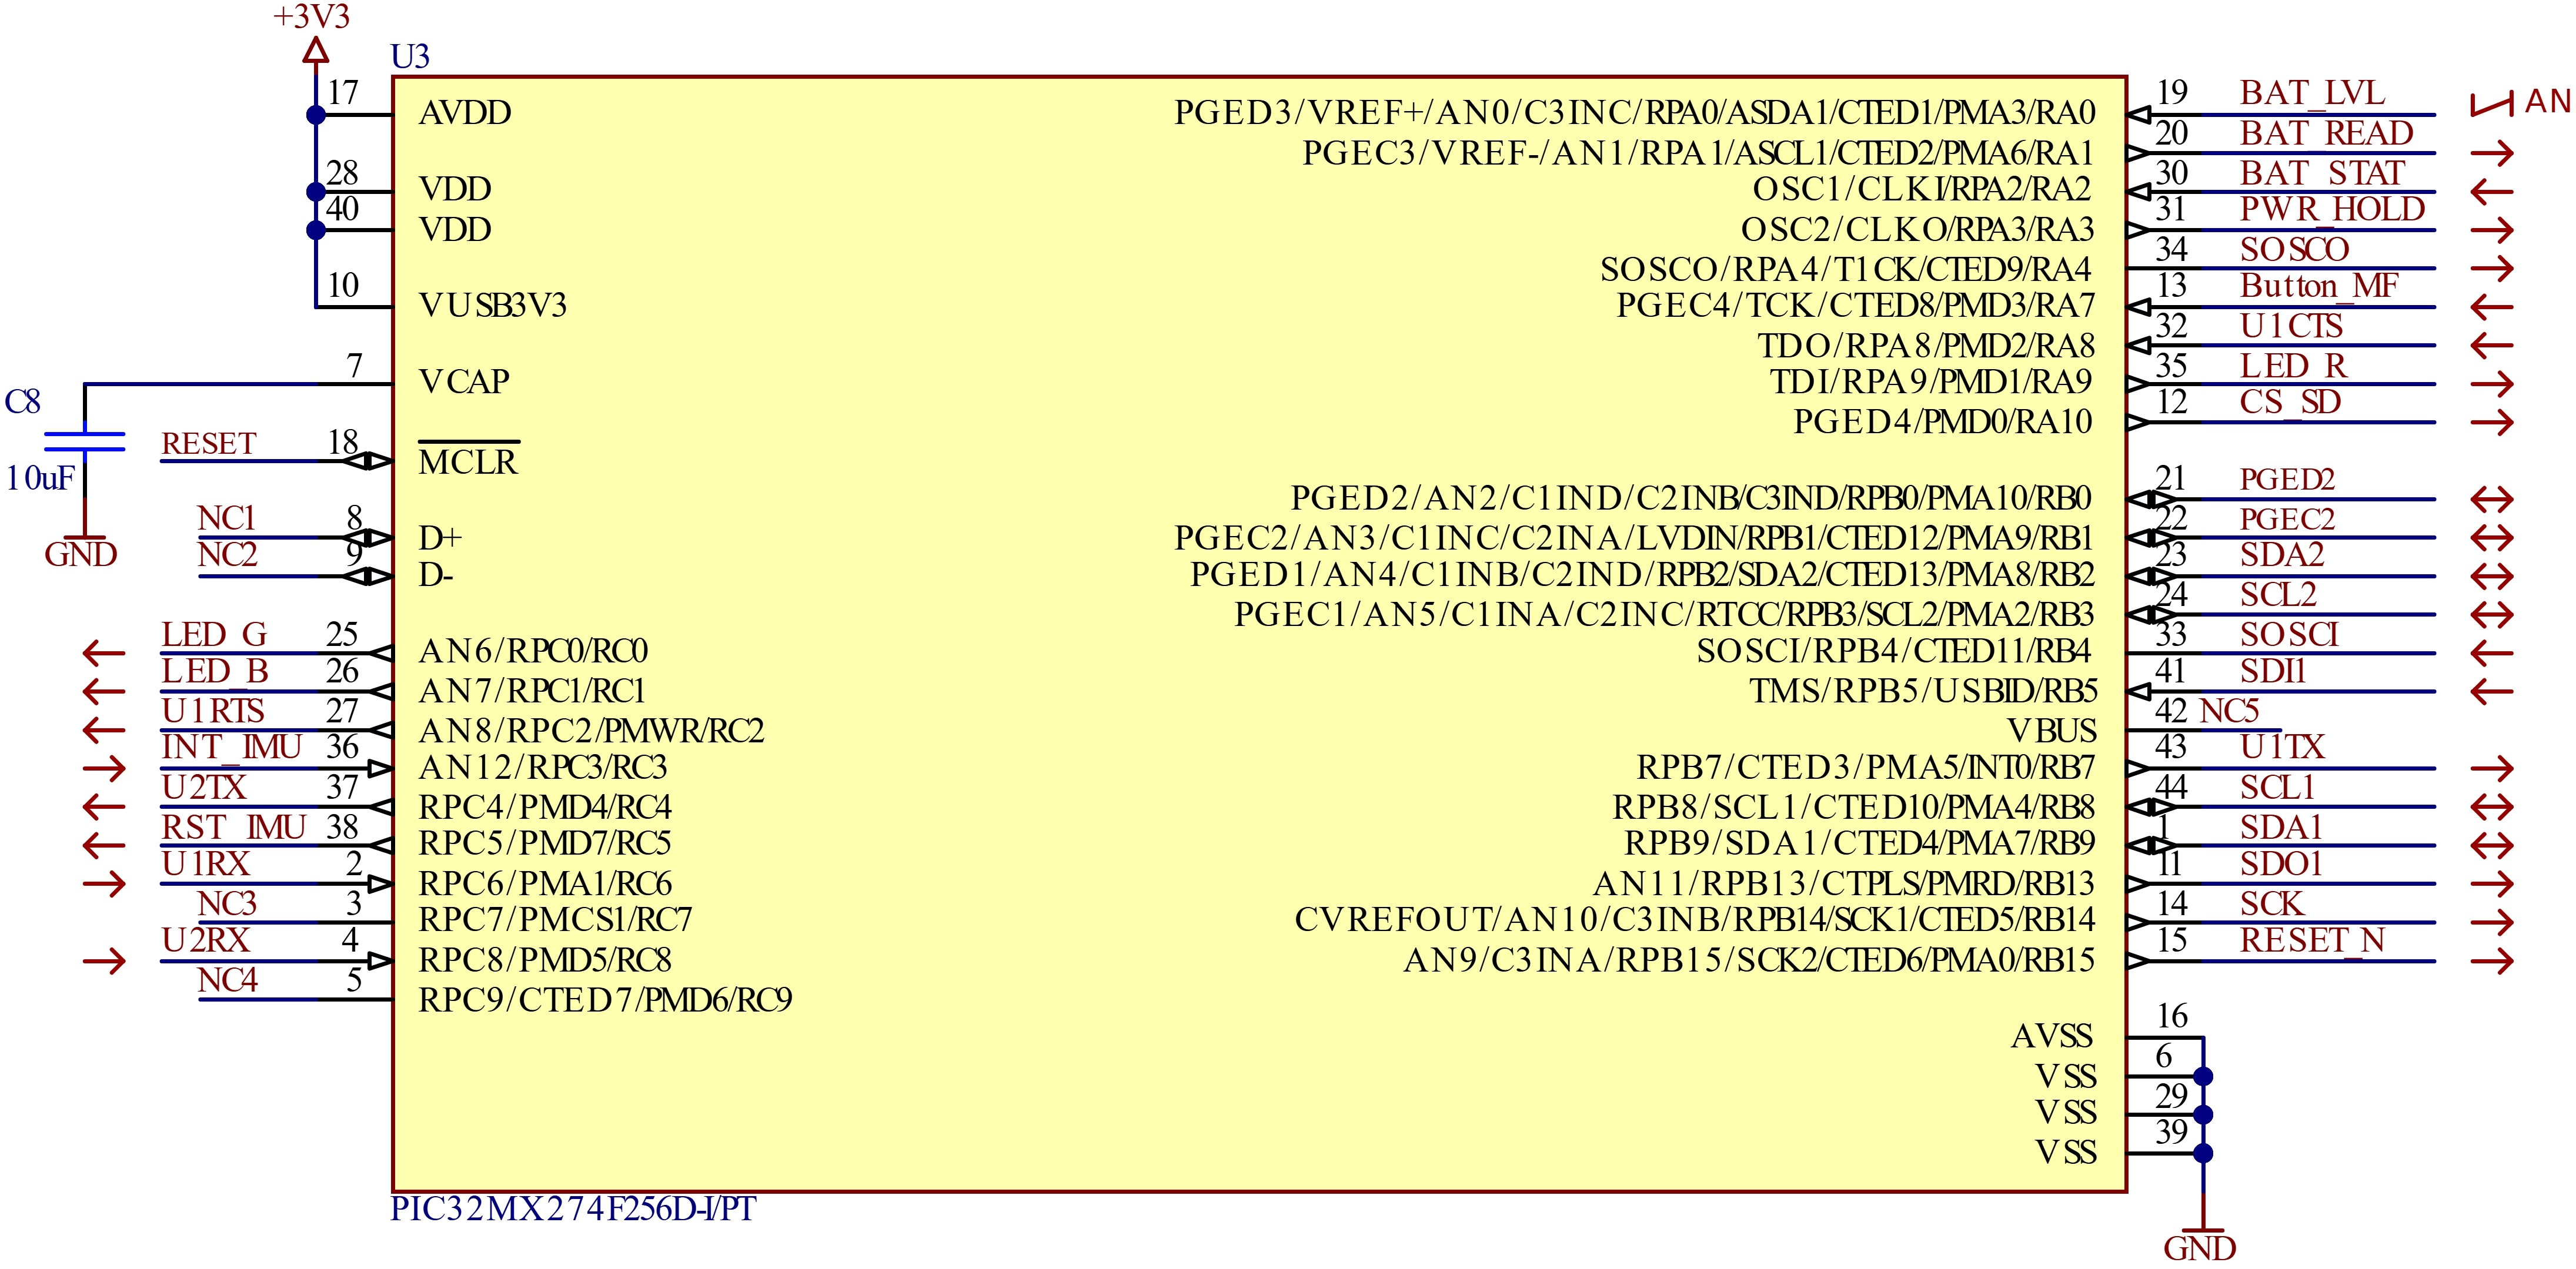
\includegraphics[width=1\linewidth]{../figures/etude/sch/MCU}
		\caption{Connexions du microcontrôleur}
		\label{fig:mcu}
	\end{subfigure}
	\hfill
	\begin{subfigure}[b]{0.3\textwidth}
		\centering
		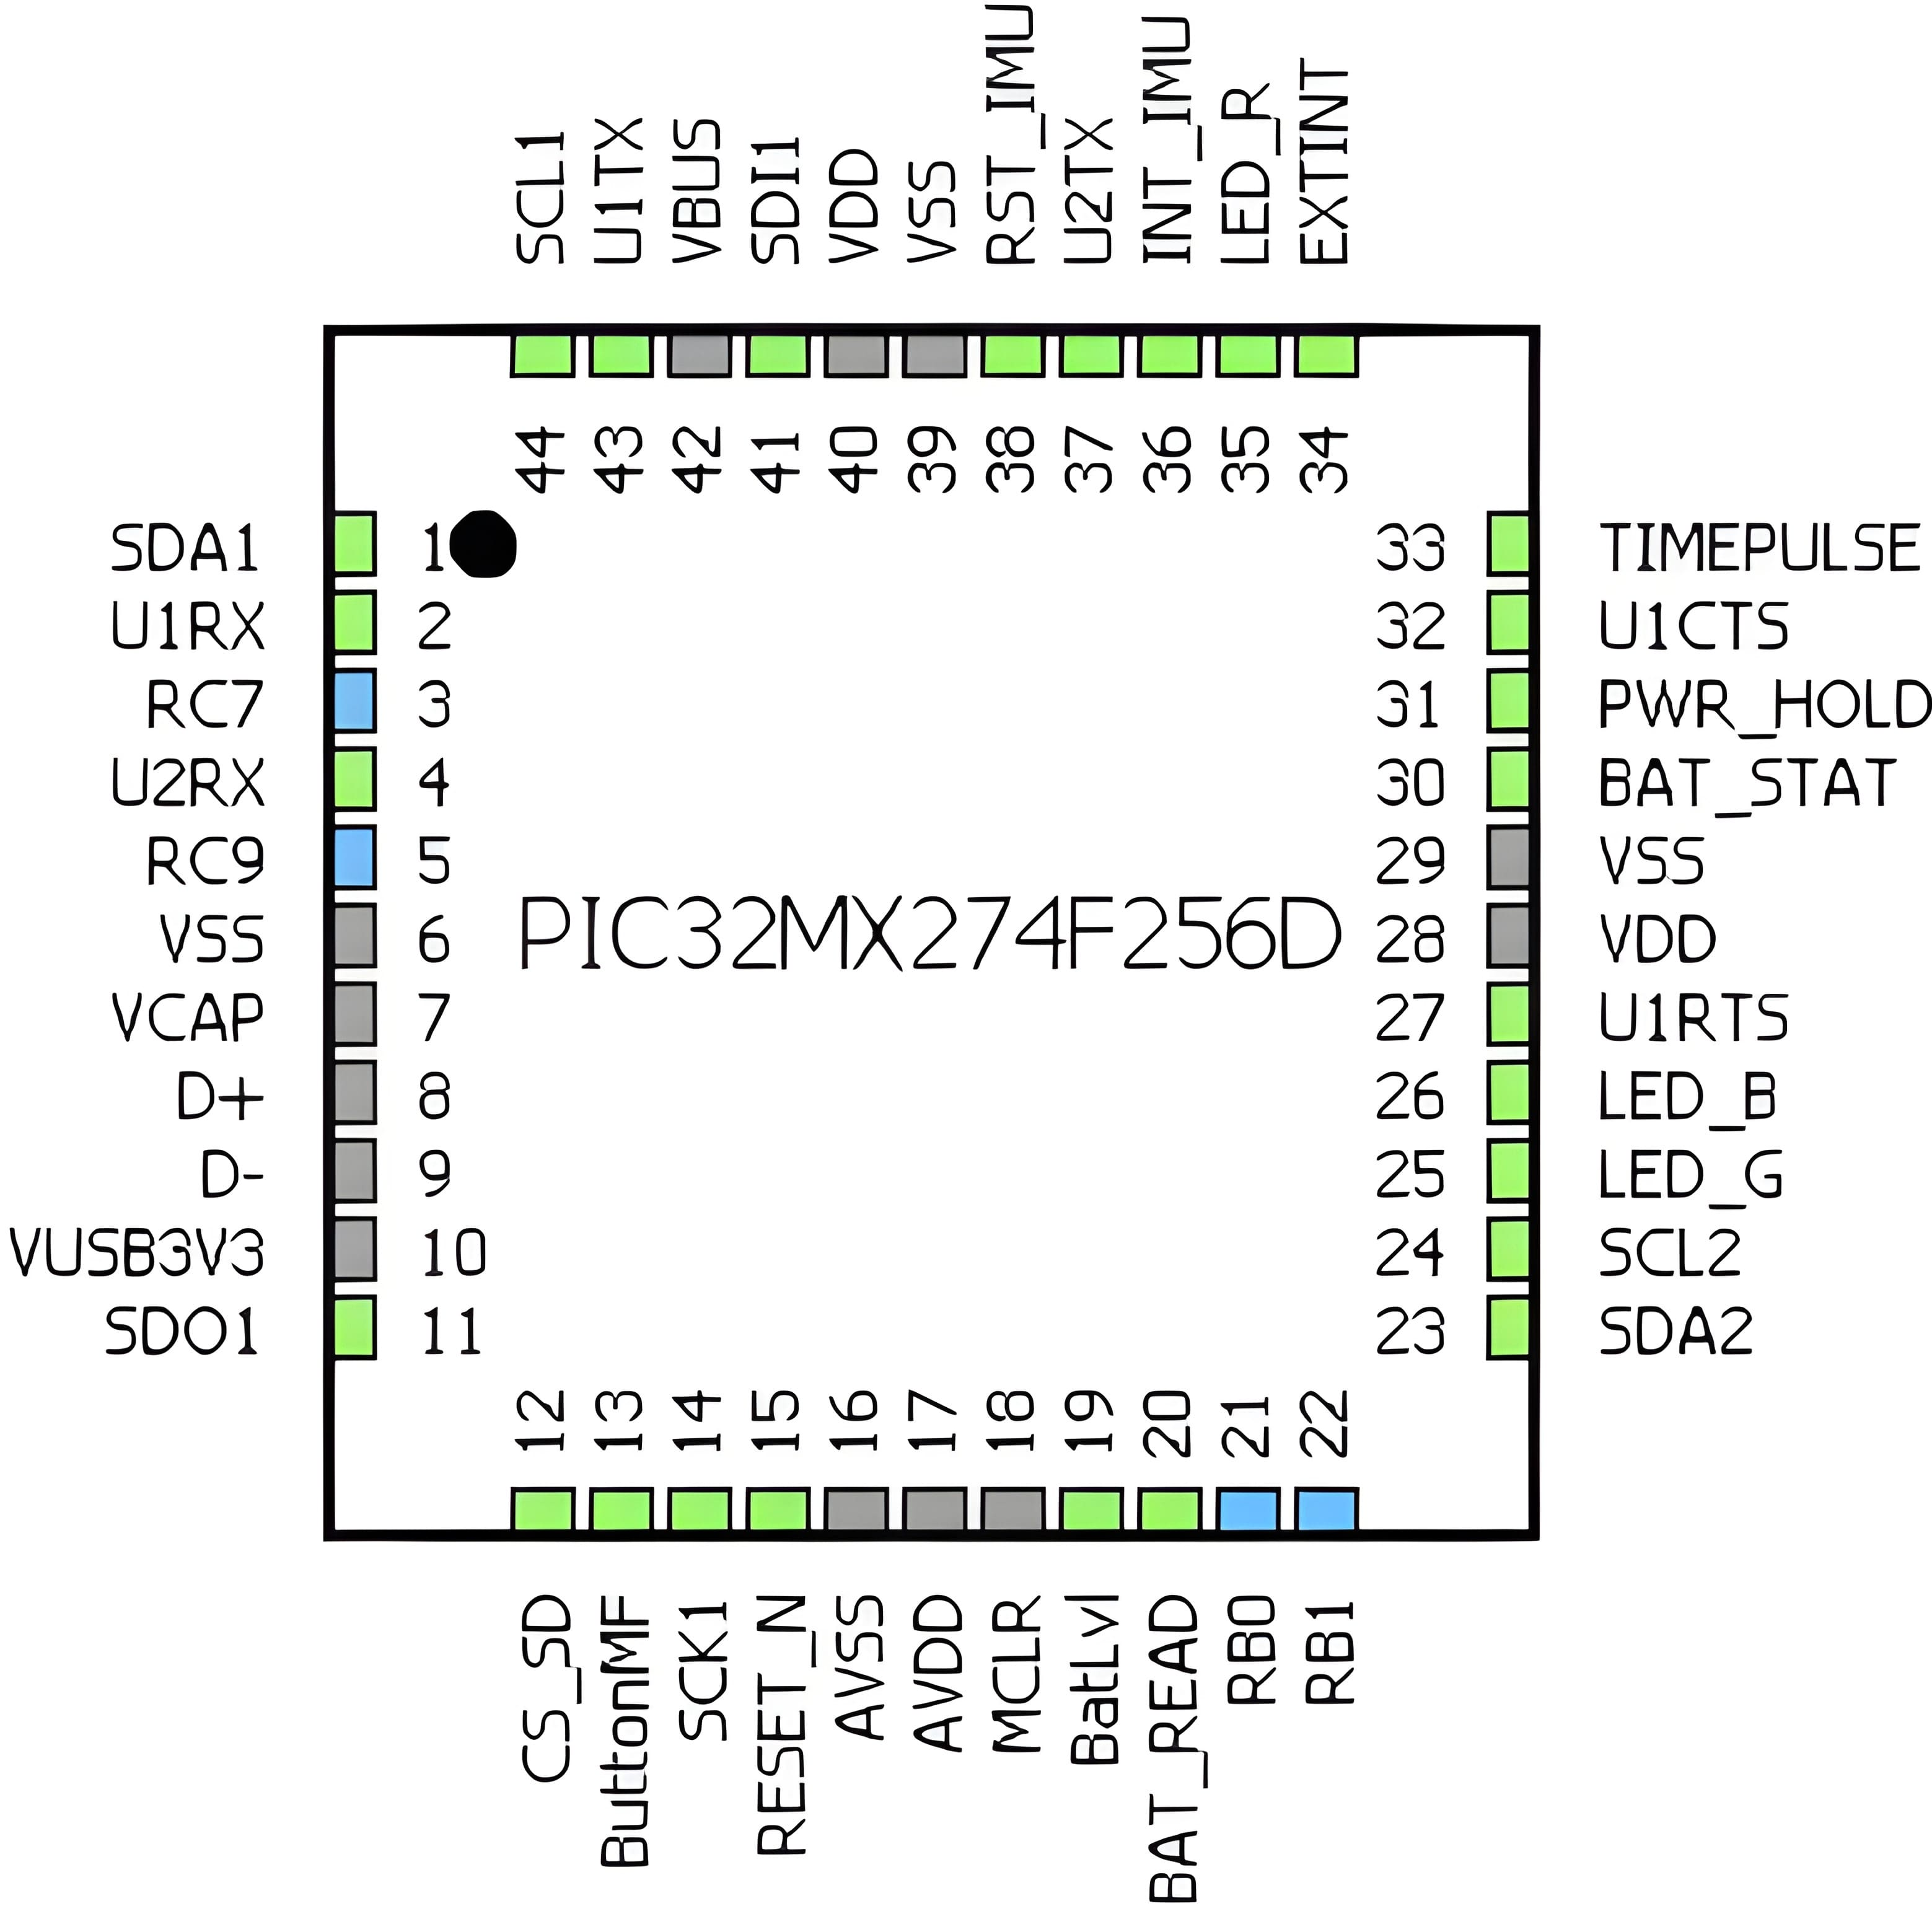
\includegraphics[width=1\linewidth]{../figures/etude/sch/MCU-HARMONY}
		\caption{Config. \gls{harmony}.}
		\label{fig:mcu-harmony}
	\end{subfigure}
	\hfill
	\caption{Configuration des PINs du microcontrôleur.}
	\source{Auteur}
	\label{fig:sch-connMcu}
\end{figure}

Pour valider les connexions de la figure \ref{fig:mcu}, une vérification a été réalisée à l'aide du configurateur graphique \gls{harmony}, comme le montre la figure \ref{fig:mcu-harmony}. Cette étape a confirmé la possibilité d'attribuer certaines fonctions à des PINs spécifiques. Les PINs non utilisées du microcontrôleur sont redirigées vers un connecteur. Dans le contexte du prototype, cela permet de les exploiter ailleurs sur la carte.


\subsubsection{Programmateur et reset} 

\begin{figure}[h]
	\centering
	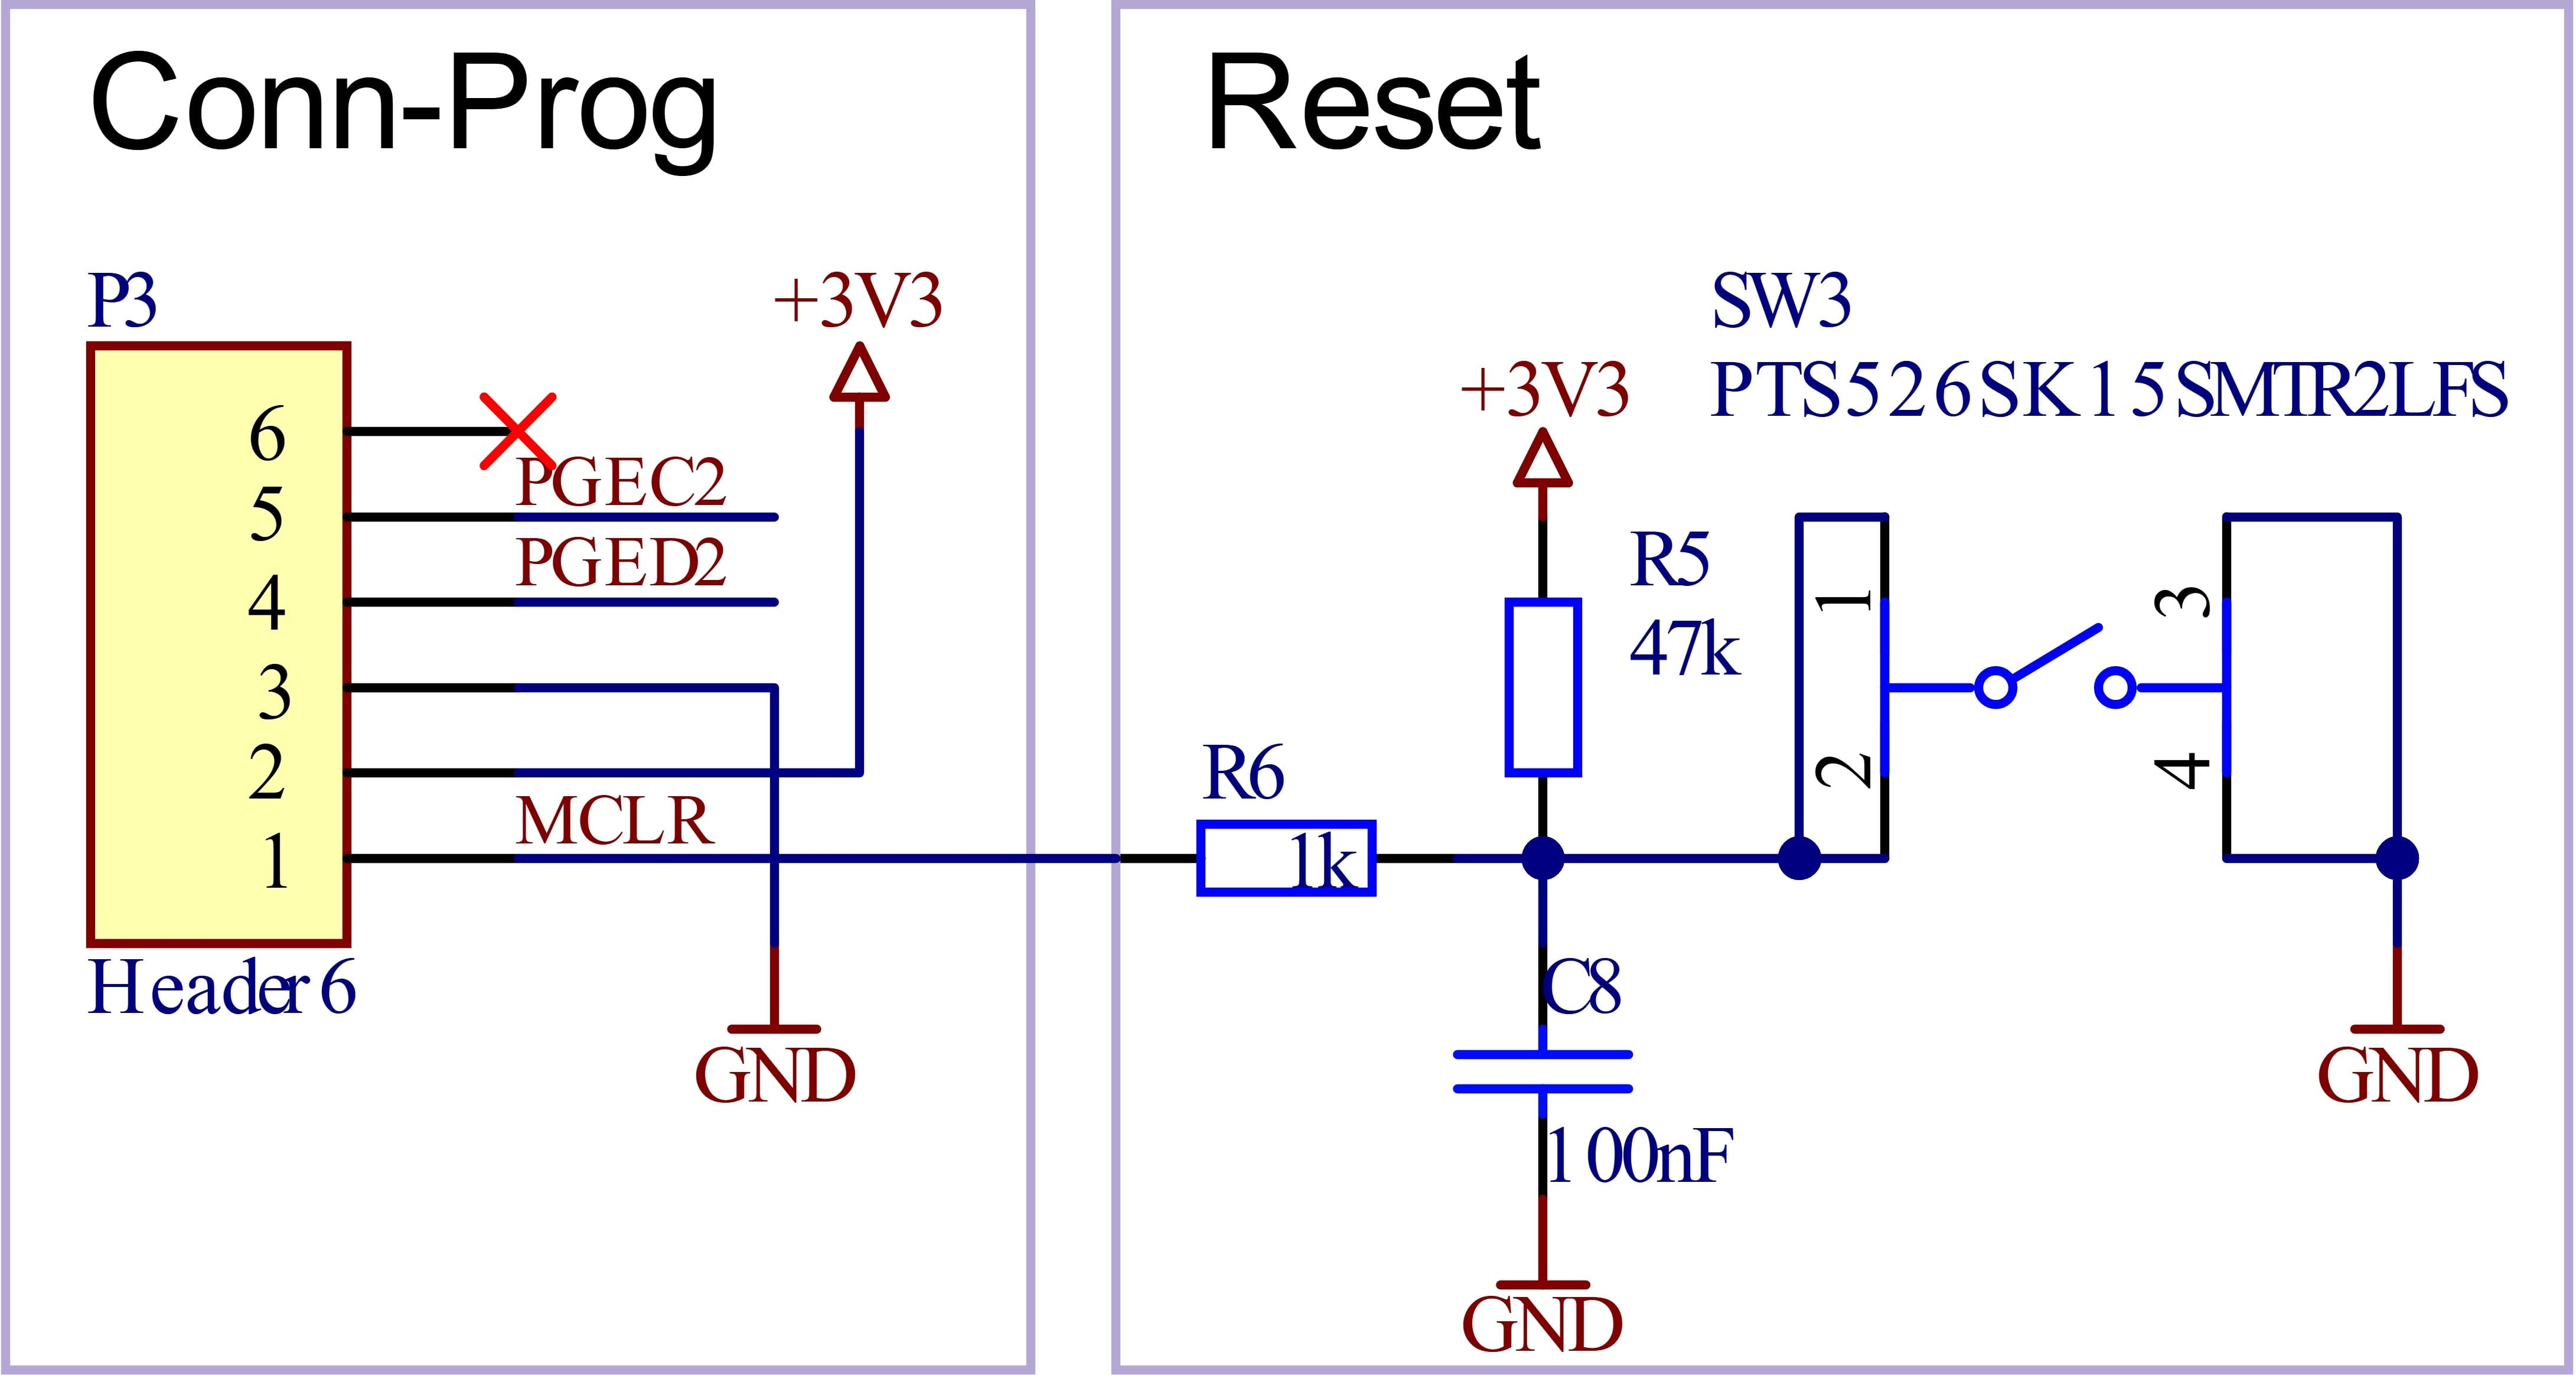
\includegraphics[width=.65\linewidth]{../figures/etude/sch/Prog-Reset}
	\caption{Schéma programmateur et reset.}
	\source{Auteur}
	\label{fig:prog-reset}
\end{figure}

Sur la figure \ref{fig:prog-reset}, nous pouvons observer le connecteur de programmation \textit{P3}. La connexion \textbf{MCLR} (Master Clear), qui permet de réinitialiser le \gls{mcu} lors de sa programmation, est suivie d'un bouton pour permettre une réinitialisation manuelle.

\clearpage

\subsubsection{LED de vie} 

\begin{figure}[h]
	\centering
	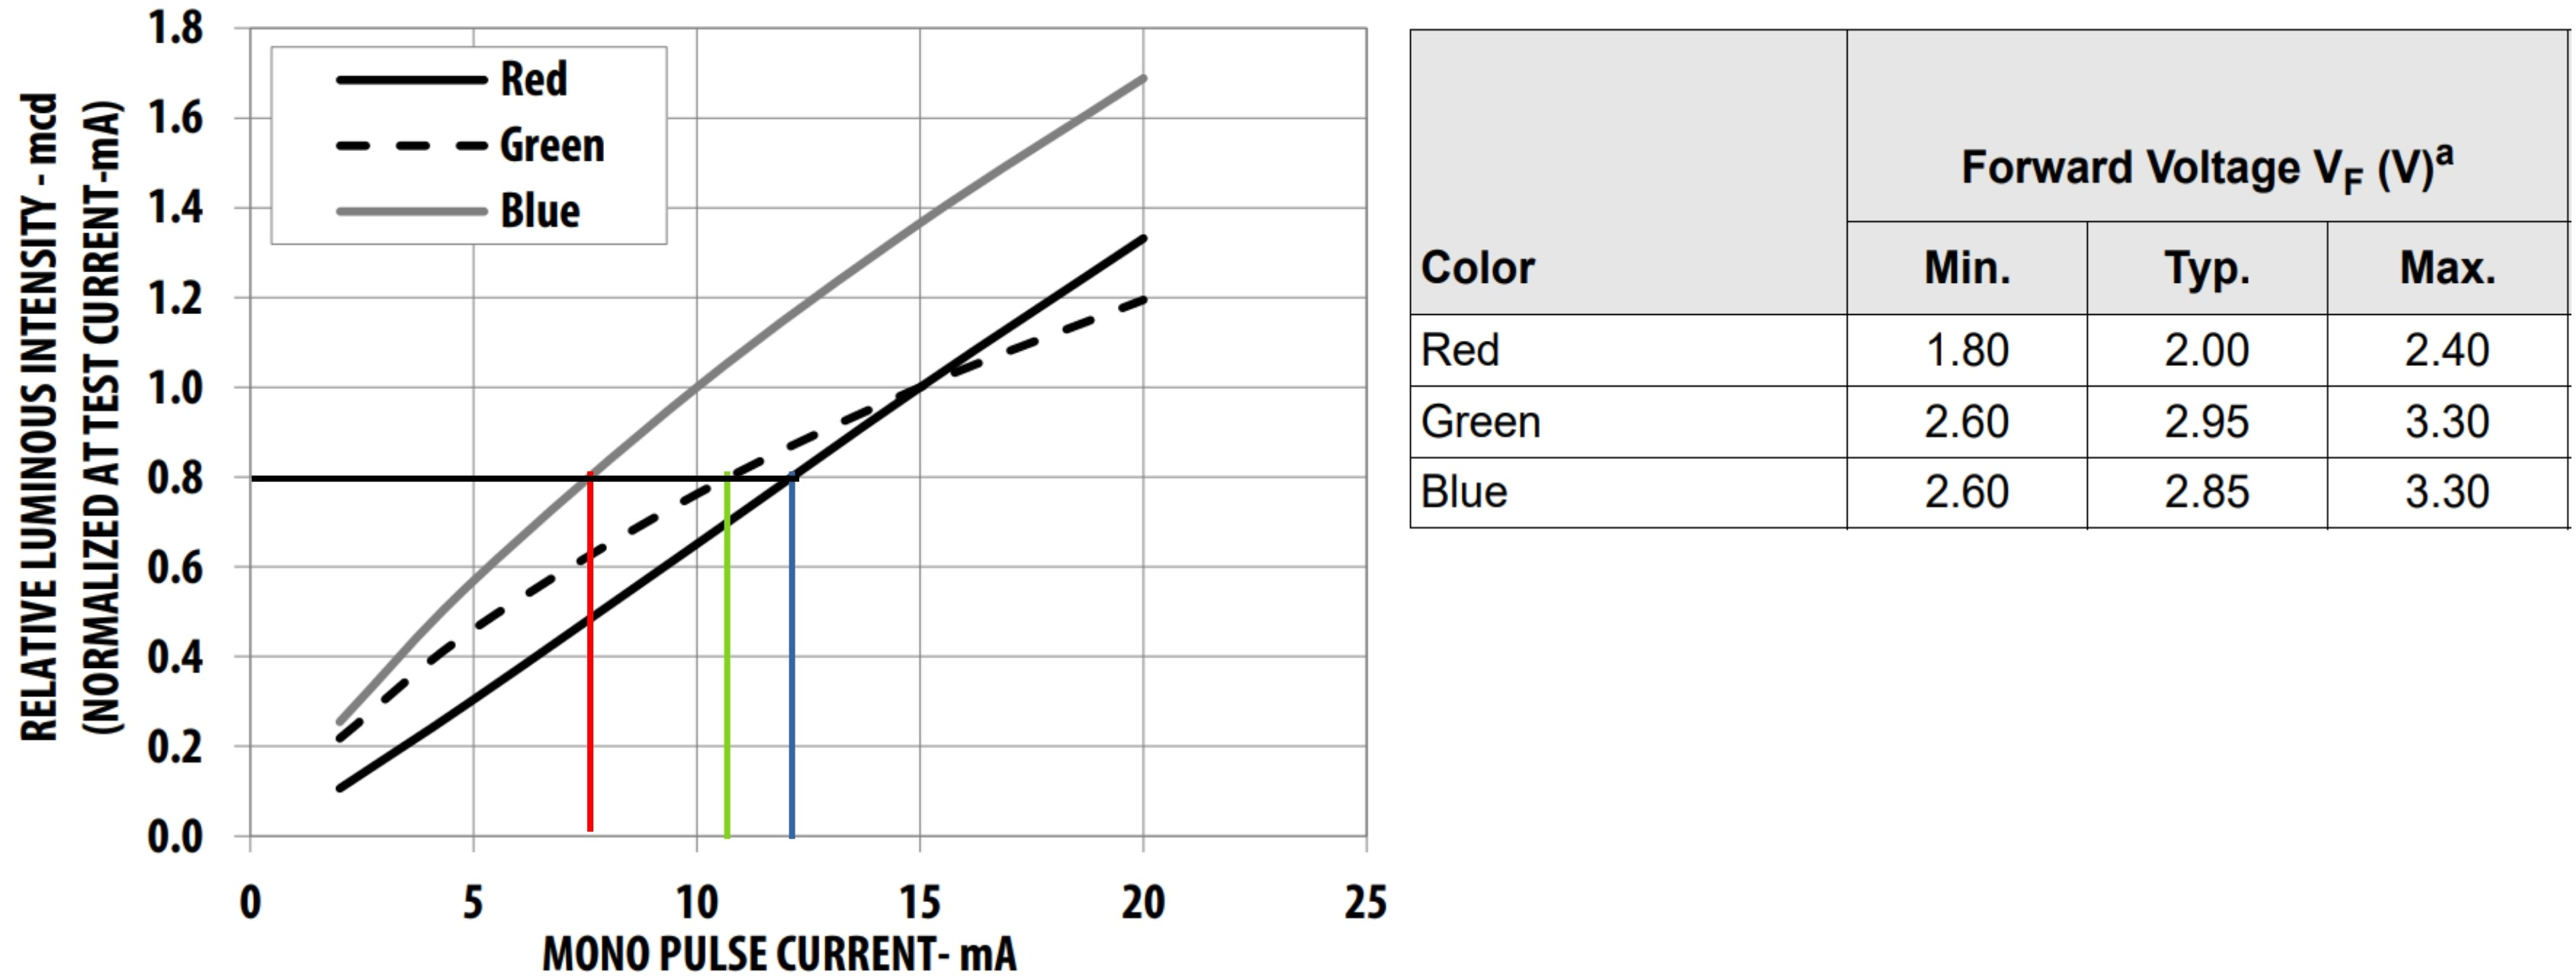
\includegraphics[width=.9\linewidth]{../figures/etude/DIM-LED}
	\caption{Données de la LED}
	\source{\gls{datasheet} \href{https://docs.broadcom.com/doc/ASMB-KTF0-0A306-DS100}{ASMB-KTF0-0A306}}
	\label{fig:dim-led}
\end{figure}

\begin{figure}[h]
	\centering
	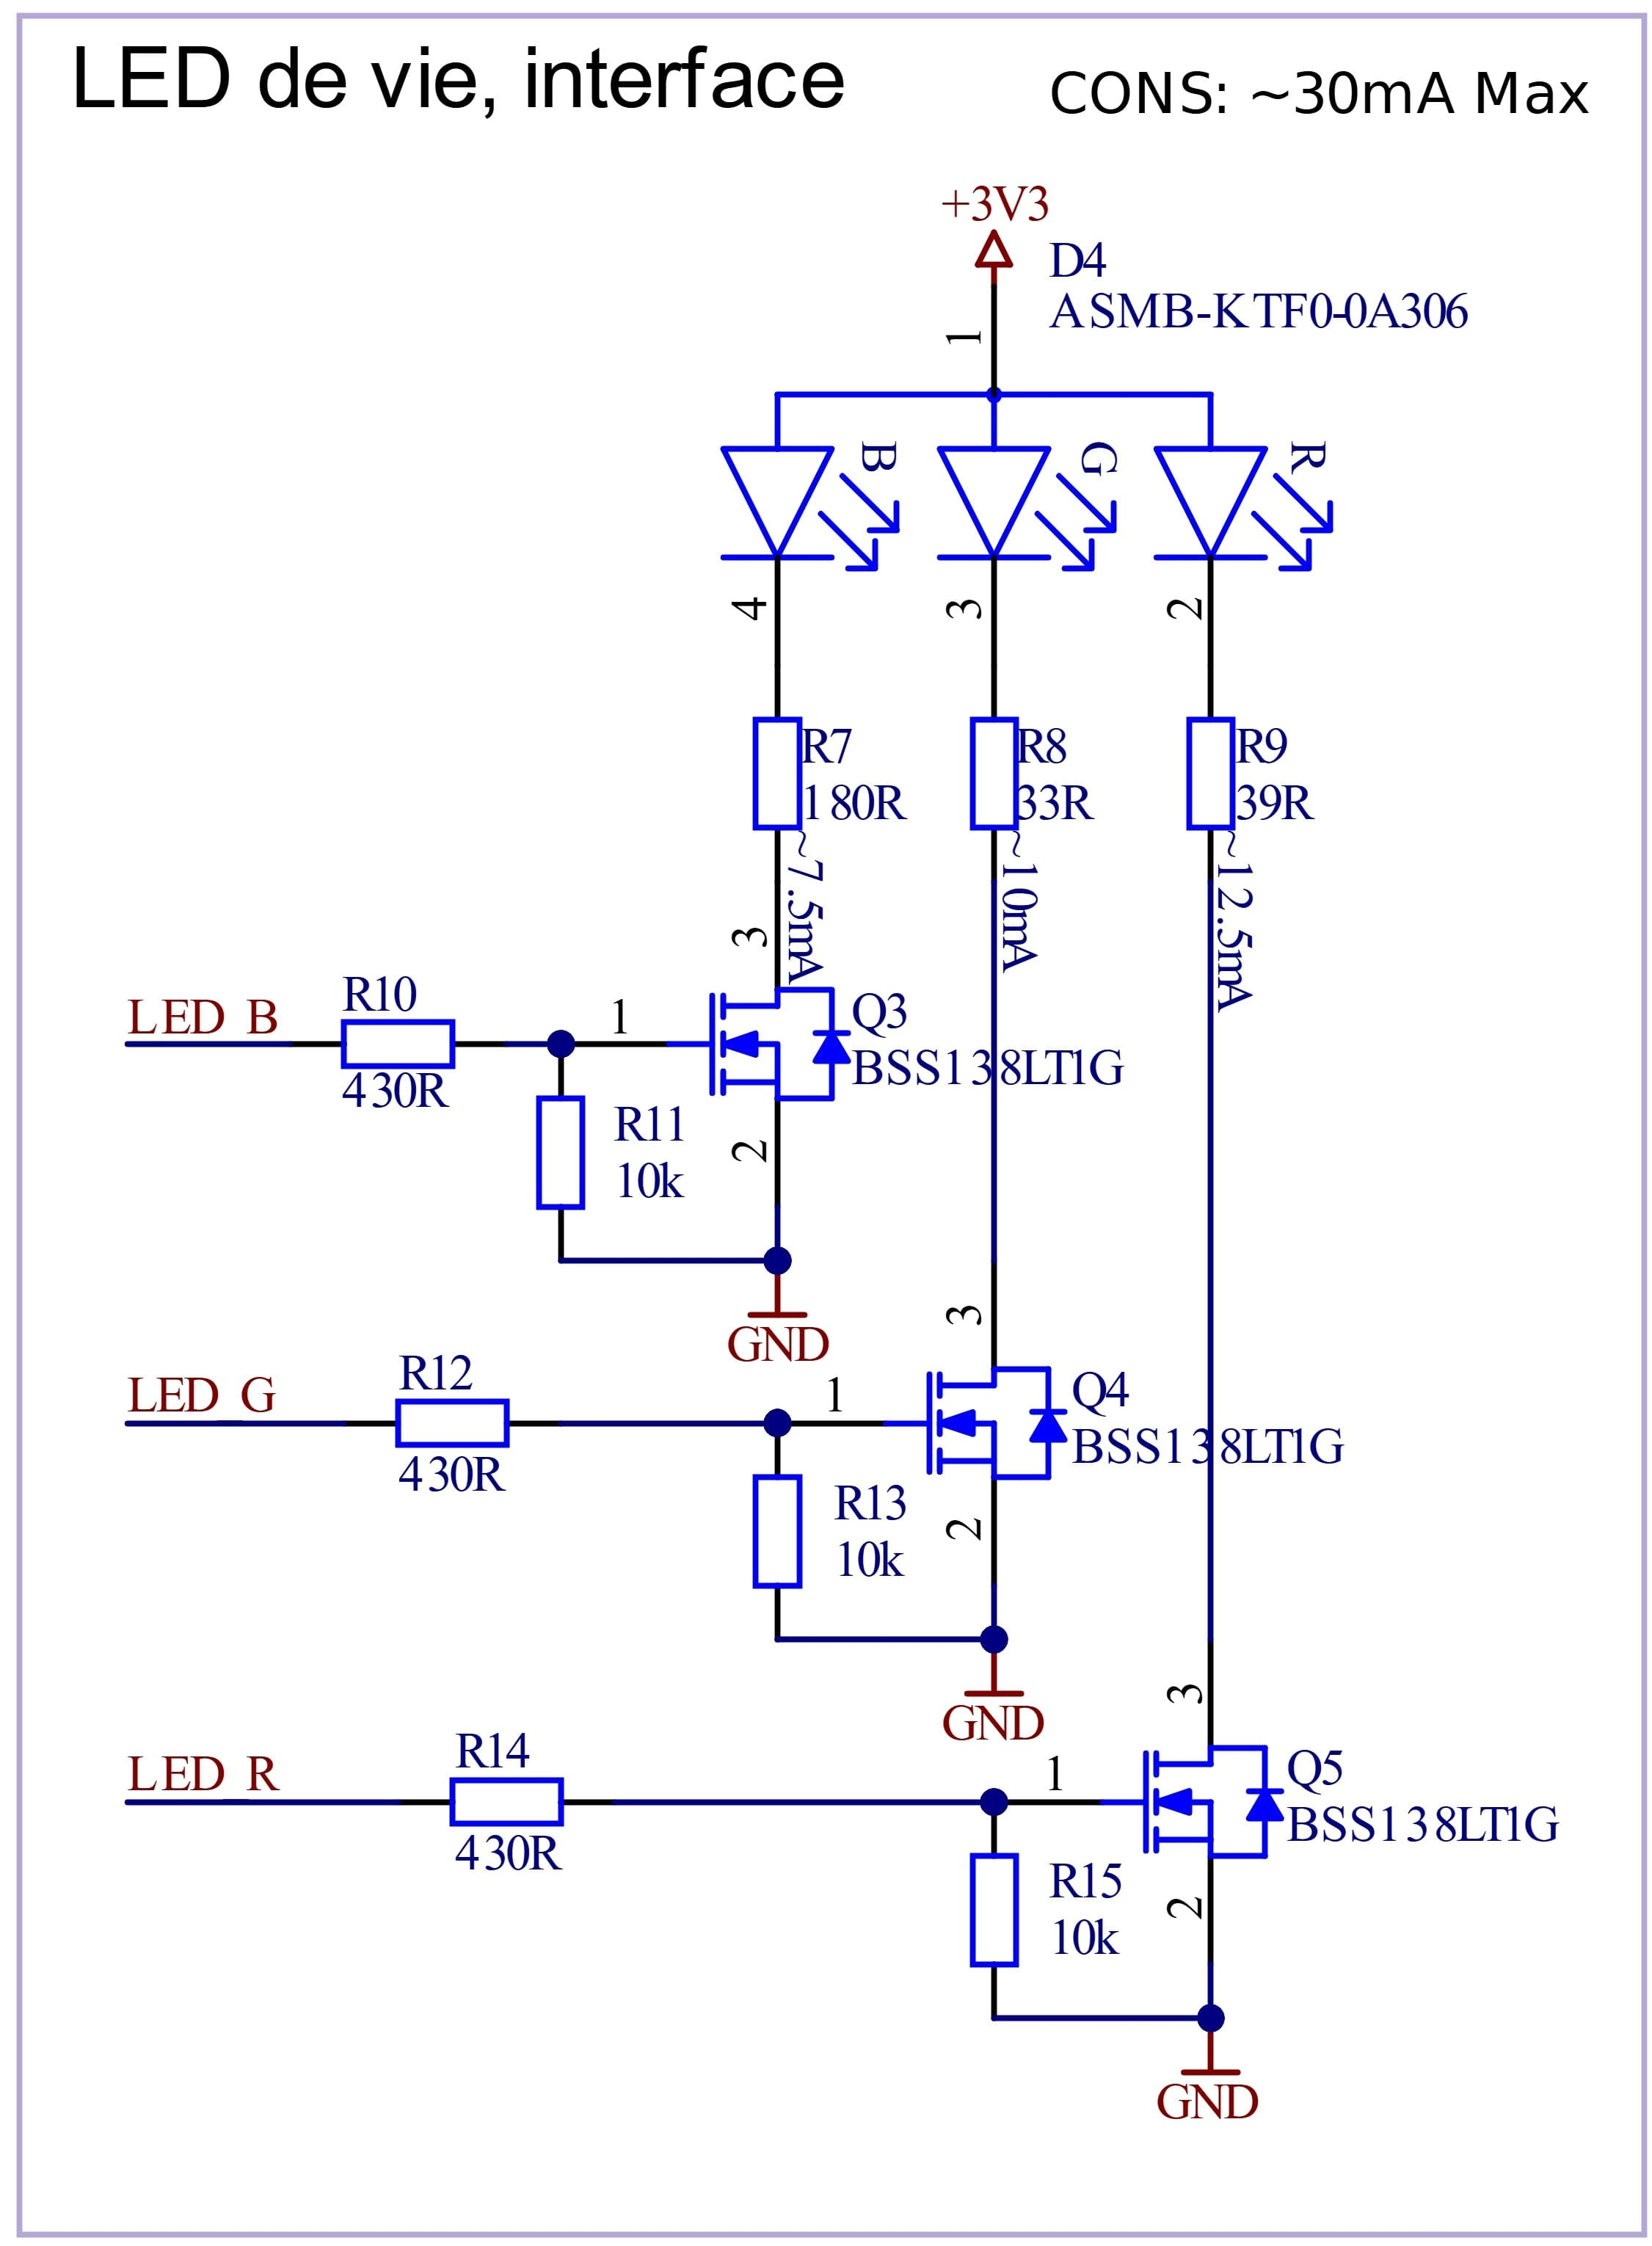
\includegraphics[width=0.4\linewidth]{../figures/etude/sch/LED-Vie}
	\caption{Schéma de la LED de vie.}
	\source{Auteur}
	\label{fig:led-vie}
\end{figure}

Les résistances de la figure \ref{fig:led-vie} ont été dimensionnées en respectant les caractéristiques des LEDs pour chacune des couleurs (voir figure \ref{fig:dim-led}). Ces dernières éclairent à 80\% de leur luminosité nominale dans un souci d'économie d'énergie, leur utilité étant réduite à ce stade de prototypage.

\begin{center}
	\underline{Exemple dimensionnement résistance LED bleue}
	\begin{equation*}
		R_{blue} = \frac{(Vcc - V_{blue})}{I_b} = \frac{(3.3 - 2.85)}{12*10^-3} = 37.5 \Omega
	\end{equation*}
\end{center}

\clearpage

\subsection{Périphériques} \label{ssec:Dev-Devices}
Dans cette section, nous allons décrire les schématiques des périphériques du système.
 
\subsubsection{Carte SD}

\begin{figure}[h]
	\centering
	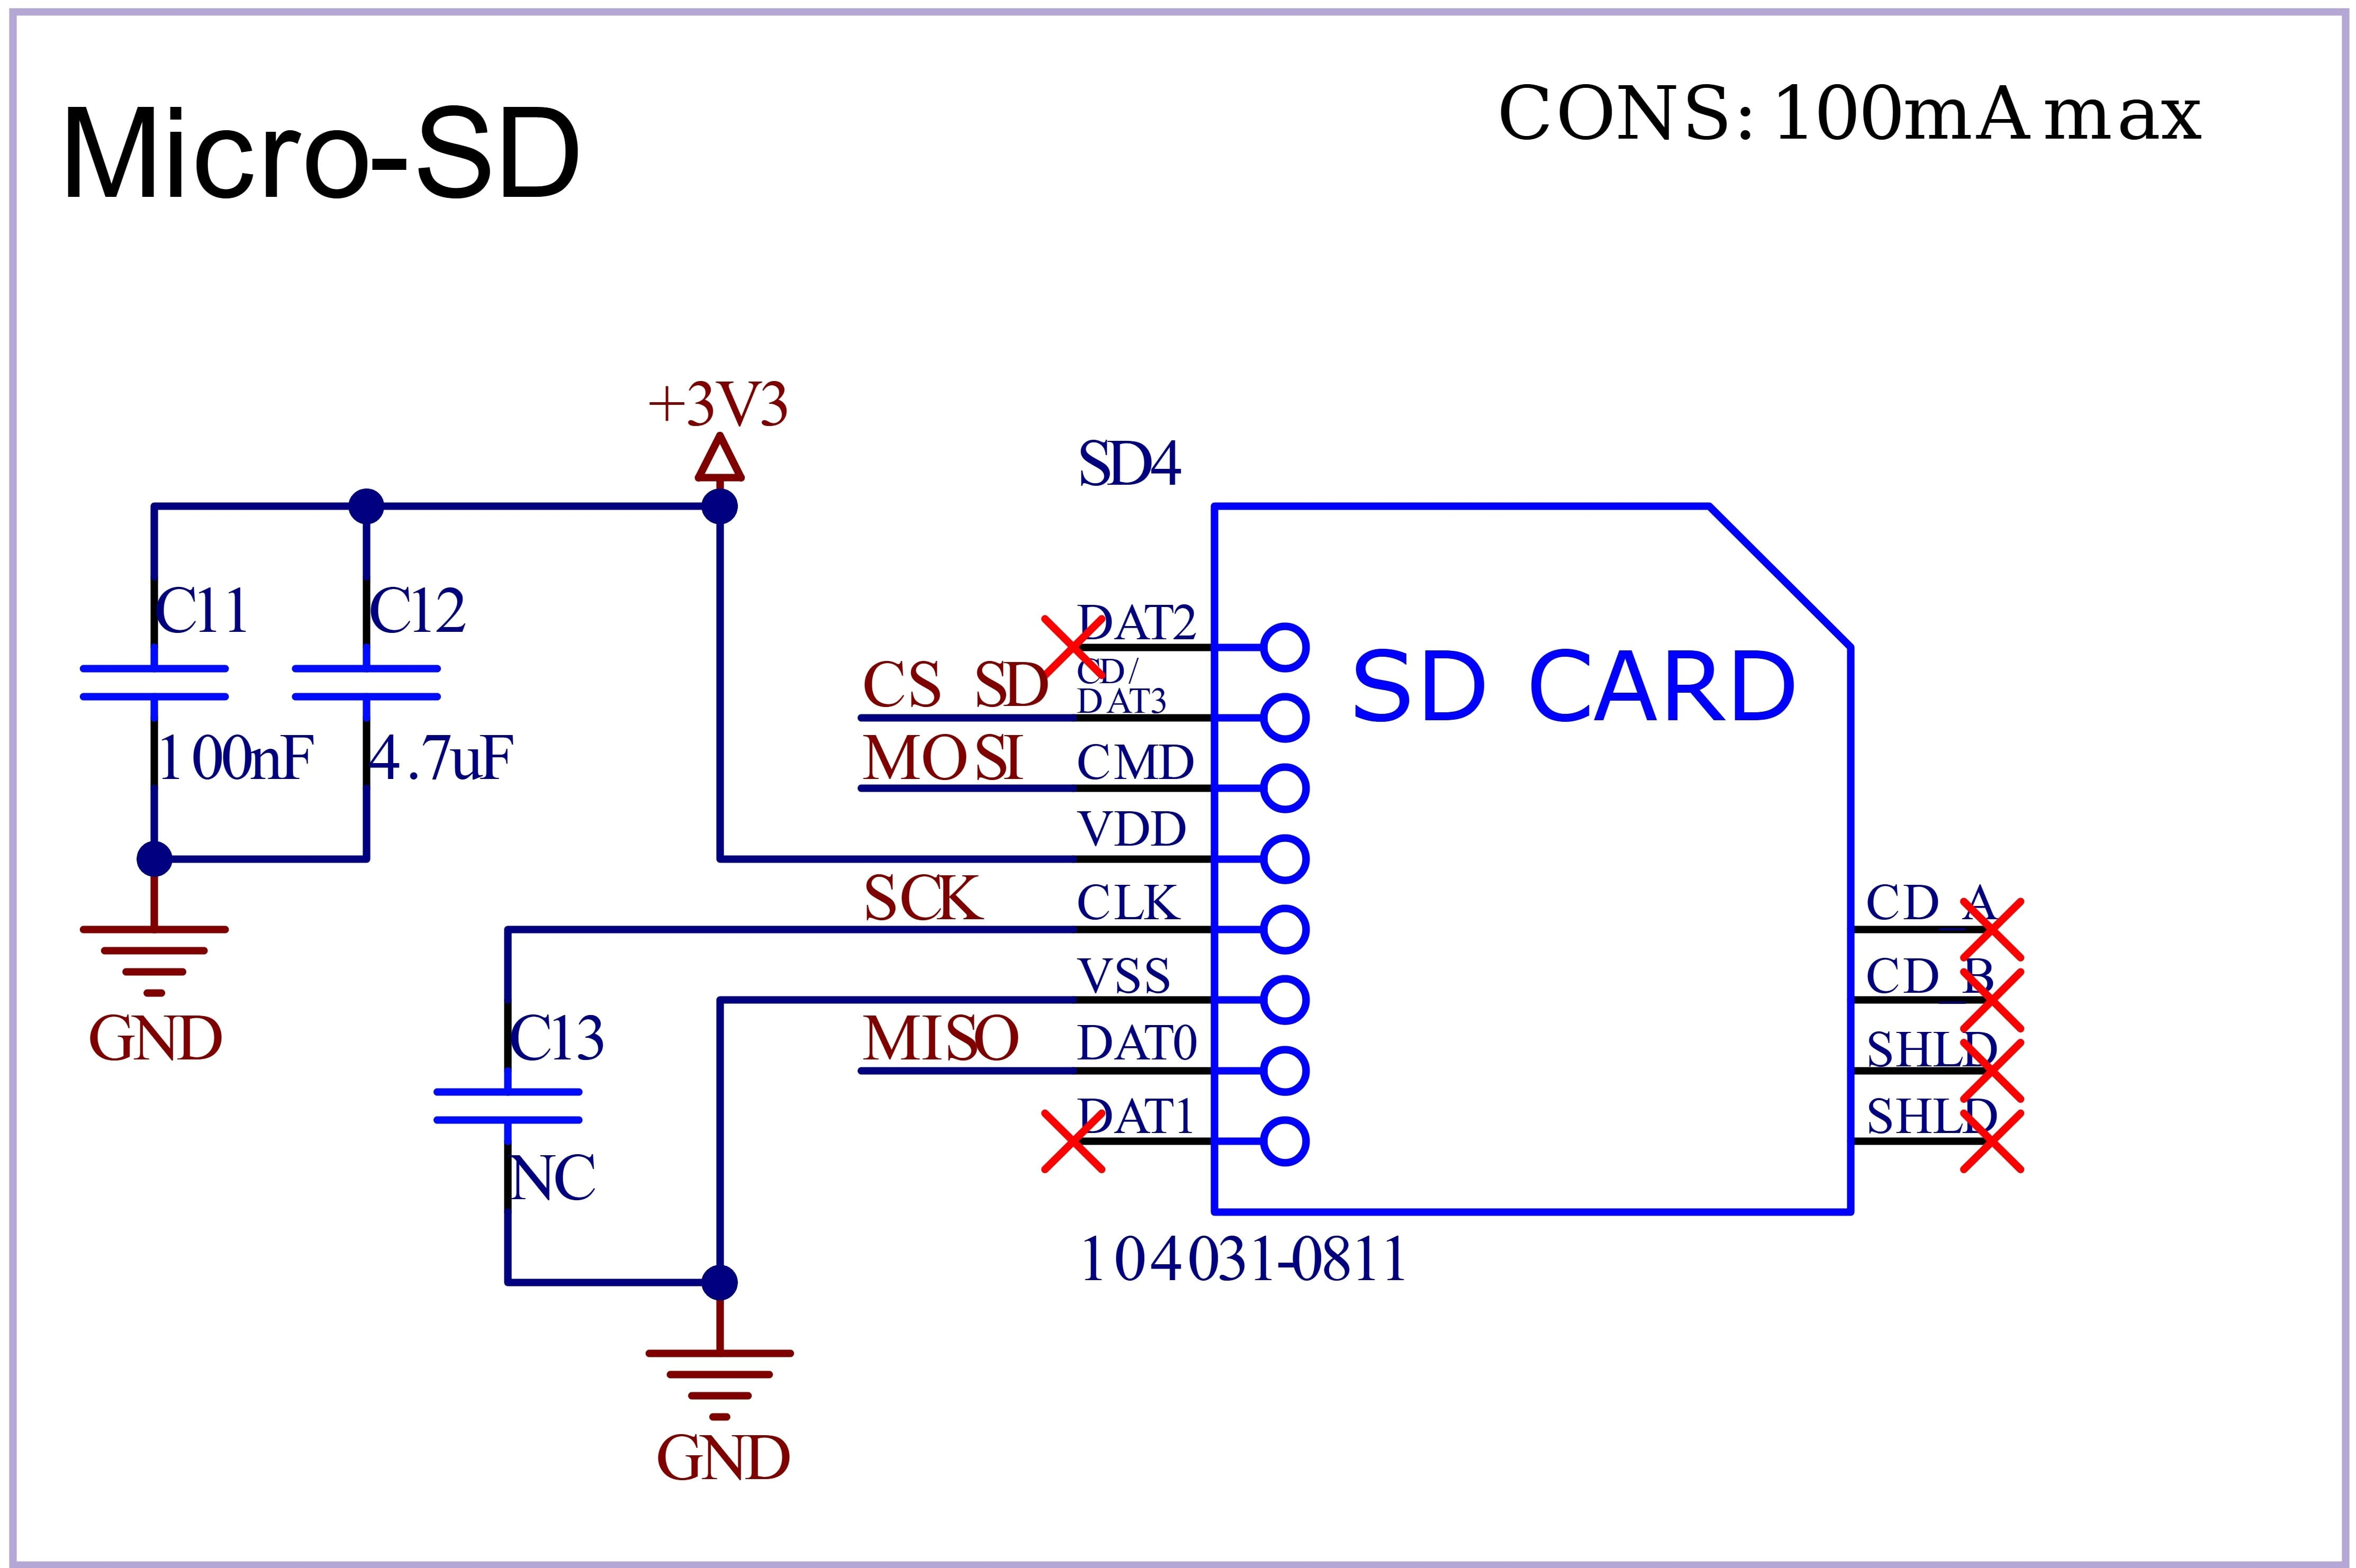
\includegraphics[width=0.5\linewidth]{../figures/etude/sch/Carte-SD}
	\caption{Branchement carte SD.}
	\source{Auteur}
	\label{fig:carte-sd}
\end{figure}

La carte SD de la figure \ref{fig:carte-sd} est branchée en respectant la connectique pour une communication SPI simple. De plus, un condensateur est connecté entre \textbf{SCK} et \textbf{GND}. Toutefois, ce condensateur ne sera pas monté sauf si un filtrage sur la ligne de clock s'avère nécessaire.


\subsubsection{Centrale inertielle}

\begin{figure}[h]
	\centering
	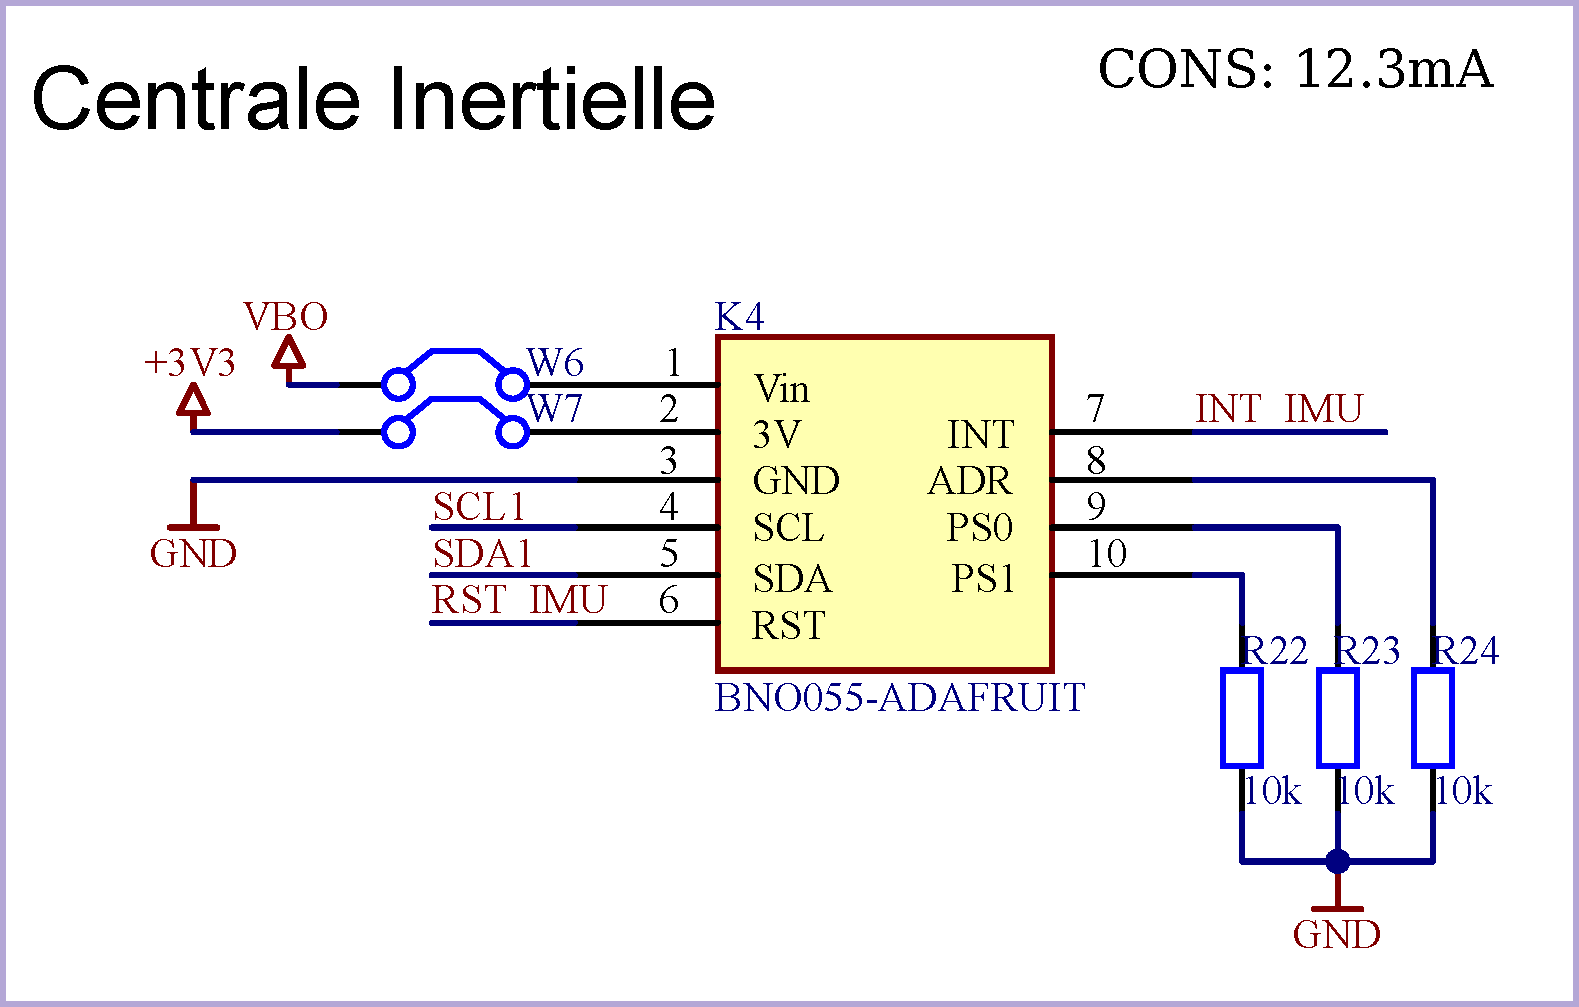
\includegraphics[width=0.5\linewidth]{../figures/etude/sch/IMU}
	\caption{Schéma centrale inertielle.}
	\source{Auteur}
	\label{fig:imu}
\end{figure}

La centrale inertielle, étant déjà montée sur une carte d'extension, ne nécessite pas de composants passifs additionnels. Trois résistances de PULL-DOWN sont présentes, respectivement sur \textbf{ADR}, \textbf{PS0} et \textbf{PS1}. Elles permettent de configurer l'adresse et l'interface de communication de l'\gls{imu}. De plus, un jumper\footnote{Connecteur permettant de faire ou de rompre une connexion.} est présent sur les alimentations. Ceci permet de choisir si la centrale inertielle est alimentée indépendamment du reste du système (pour pouvoir l'allumer séparément) ou avec la même alimentation que le reste du système.


\subsubsection{GNSS}
\begin{figure}[h]
	\centering
	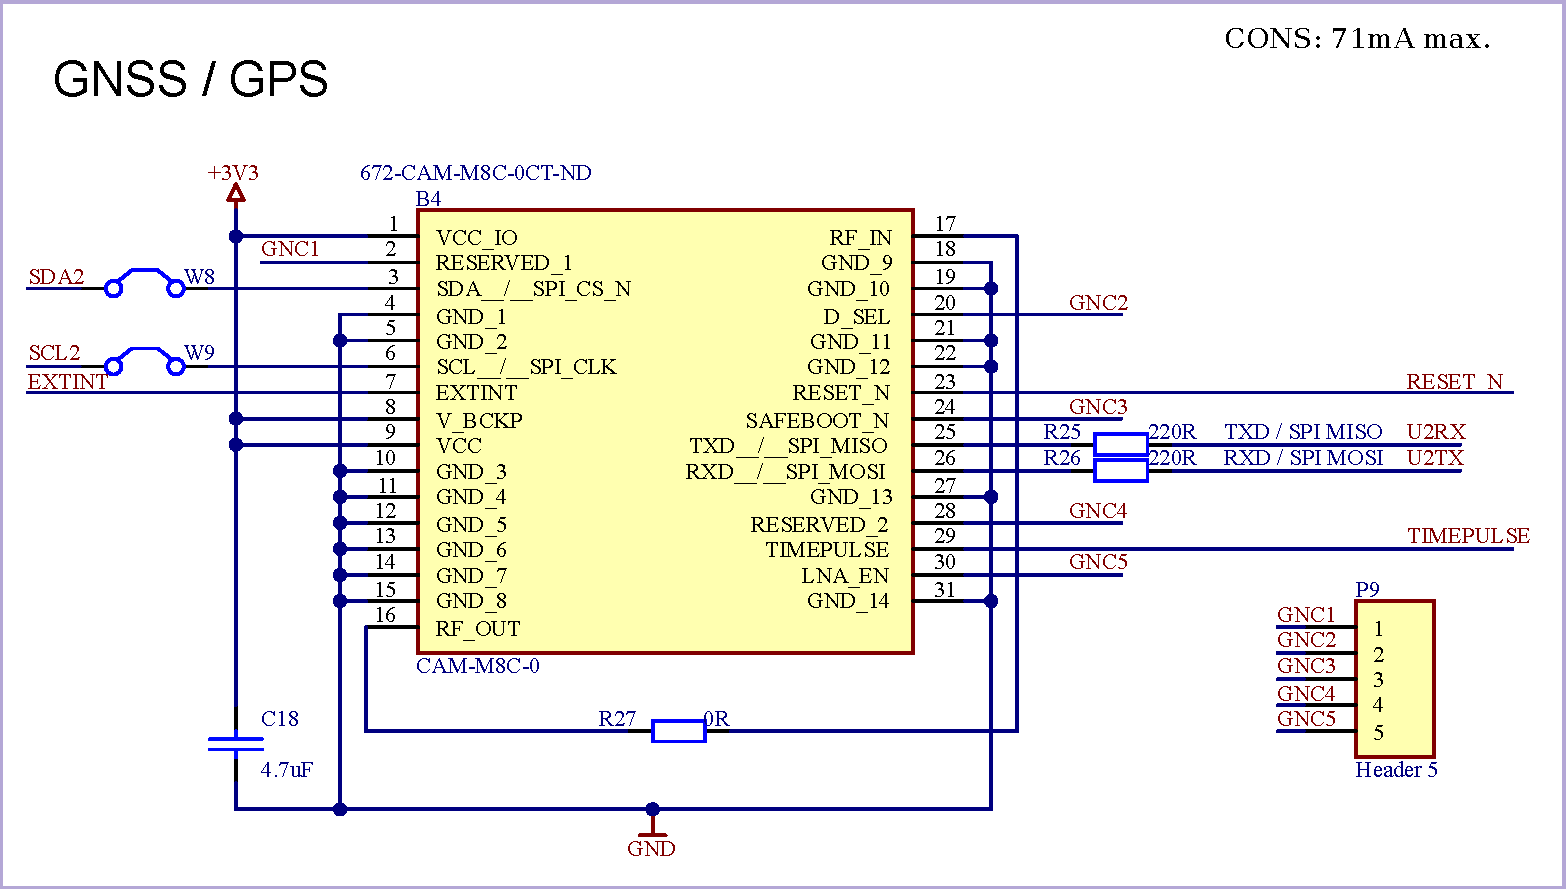
\includegraphics[width=.6\linewidth]{../figures/etude/sch/GNSS}
	\caption{Schéma du \gls{GNSS}.}
	\source{Auteur}
	\label{fig:gnss}
\end{figure}

Le \gls{GNSS} est connecté selon un schéma présenté dans son \href{https://www.u-blox.com/sites/default/files/CAM-M8-FW3_HIM_%28UBX-15030063%29.pdf}{Hardware Integration Manual}, à la section \textbf{2.2}. Ce schéma représente un design minimal pour recevoir des données via l'interface UART. Par rapport à la figure \ref{fig:gnss}, les différences sont les suivantes : l'interface I2C est également disponible, la PIN \textbf{RESET\_N} est connectée au \gls{mcu} et les PINS non-utilisées sont reliées à un connecteur afin de permettre leur utilisation éventuelle dans le cadre du prototype.

\subsubsection{USB - FTDI}

\begin{figure}[h]
	\centering
	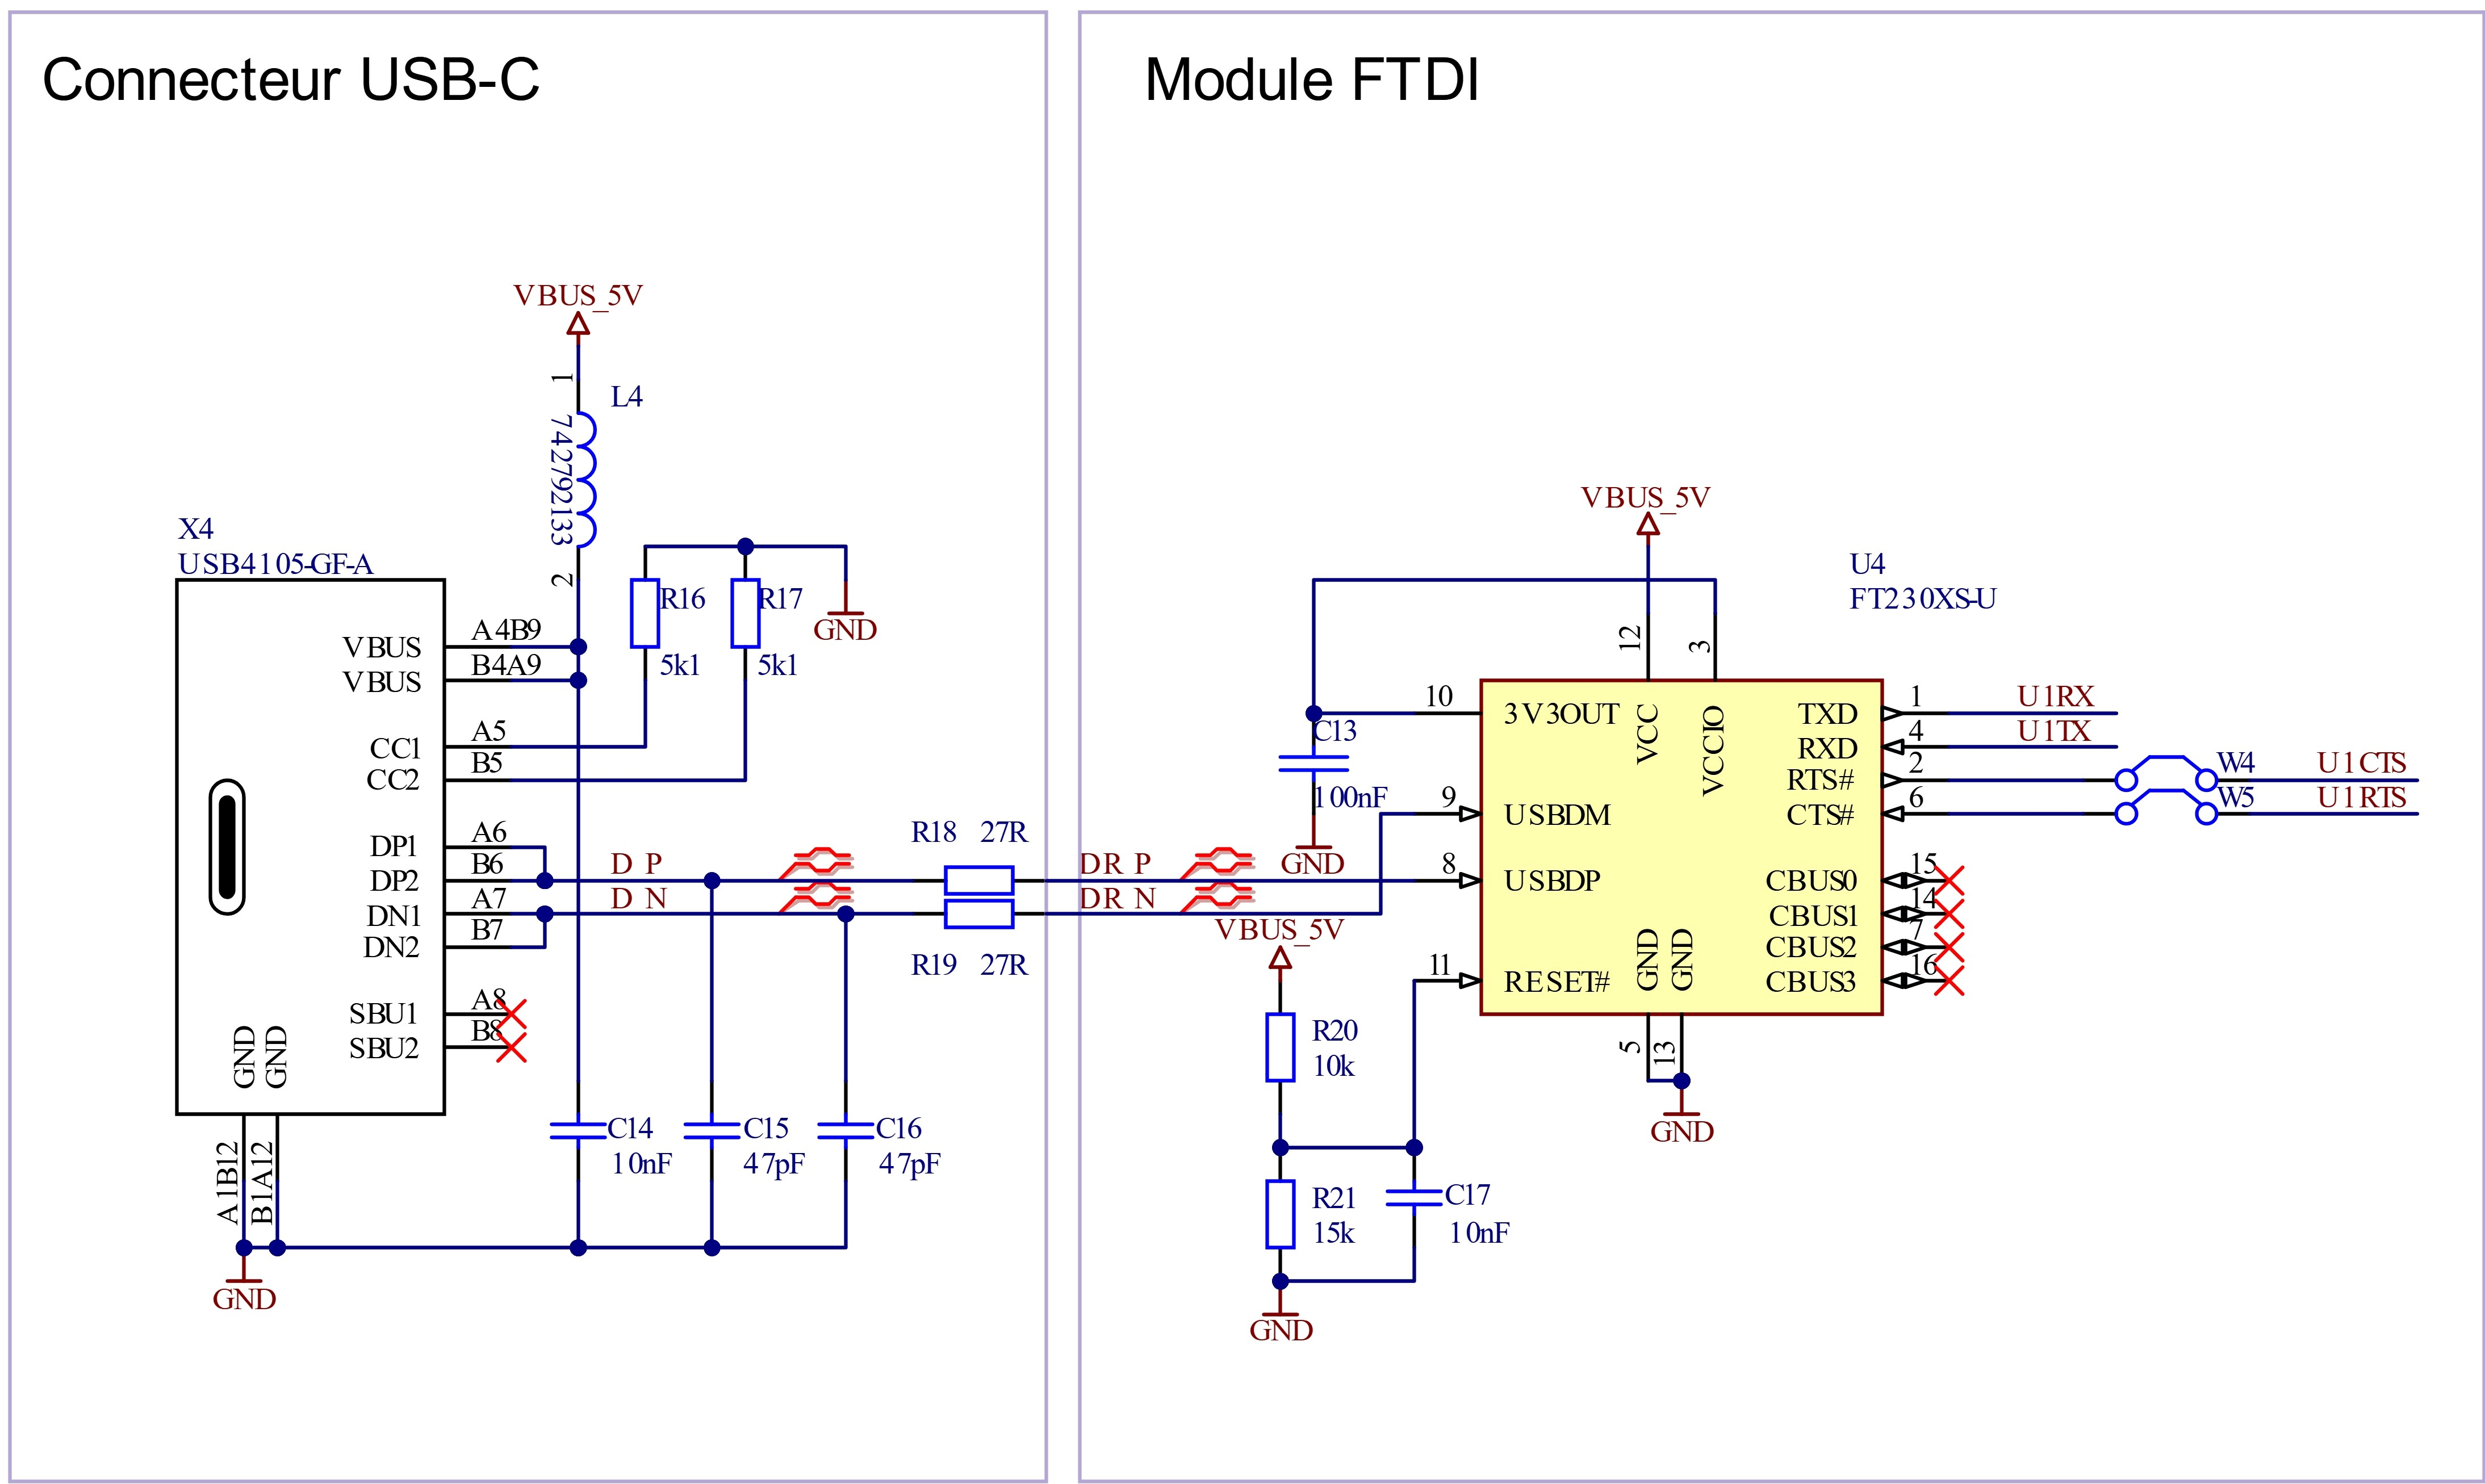
\includegraphics[width=.8\linewidth]{../figures/etude/sch/USB-FTDI}
	\caption{Schéma connecteur USB et FTDI.}
	\source{Auteur}
	\label{fig:usb-ftdi}
\end{figure}

Le schéma du connecteur USB-C est conçu pour présenter une résistance aux interférences. Son signal 5V est filtré par une \textit{ferrite bead}. Les pistes différentielles de l'USB sont ensuite reliées au module \gls{FTDI}, qui est interfacé en UART et est alimenté par l'USB.

\clearpage

\subsection{Alimentations} \label{ssec:Dev-Alim}
Dans cette section, nous allons décrire les fonctionnement et dimensionnements principaux du bloc alimentation comprenant les différents régulateurs et la batterie.

\subsubsection{Chargeur de batterie} \label{sssec:Chargeur-bat}

\begin{figure}[h]
	\centering
	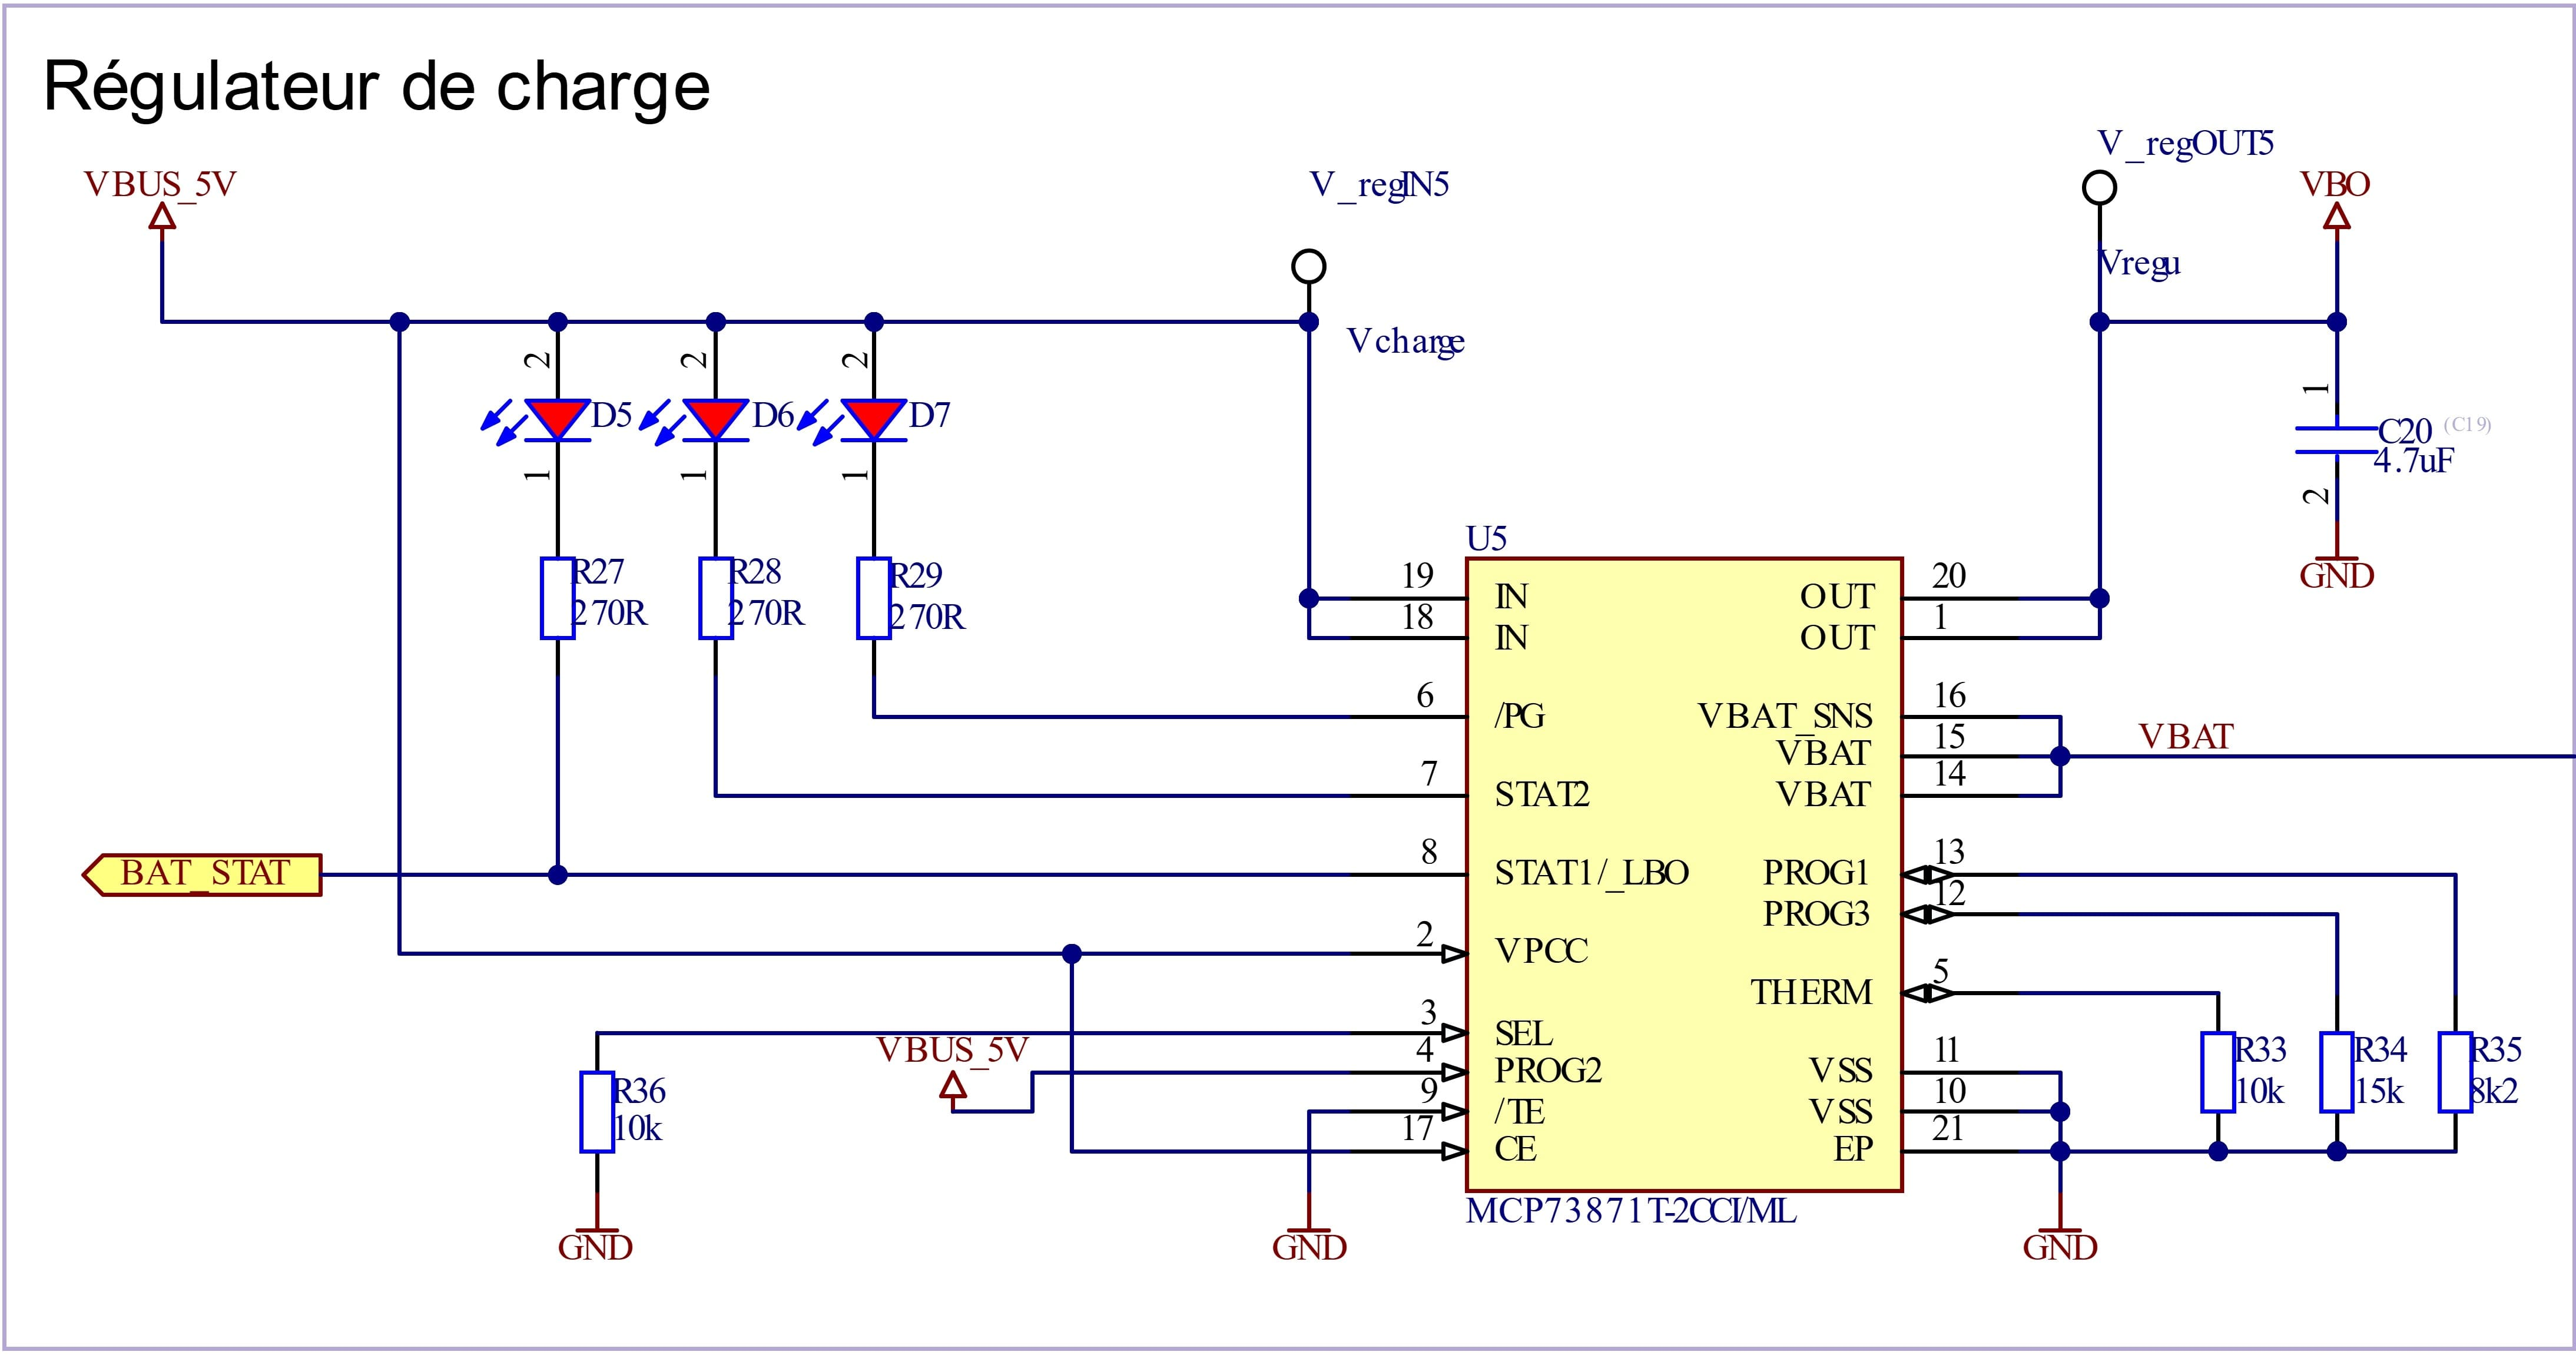
\includegraphics[width=.93\linewidth]{../figures/etude/sch/CHRG-BAT}
	\caption{Schéma chargeur de batterie.}
	\source{Auteur}
	\label{fig:chrg-bat}
\end{figure}

Le composant \textbf{MCP73871T-2CCI/ML} est configurable pour délivrer un courant de charge programmable à la batterie. Ce courant se sépare en deux phases : la charge normale et la charge de terminaison. Cette dernière est activée lorsque la batterie approche de sa capacité maximale. Pour déterminer ces courants, il convient de se baser sur la capacité de la batterie et de certains ratios standards associés.

Où :

$C = 1300 mAh$ est la capacité de la batterie.

$k_{term} = 0.05$ est le ratio de fin de charge.

$k_{chg} = 0.1$ est le ratio de charge.

Le courant de terminais peut être calculé ainsi :
\begin{equation*}
	I_{term} = C * k_{term} = 1300 * 0.05 = 65 \; mA
\end{equation*}
Par conséquent, d'après la \gls{datasheet} (\href{https://ww1.microchip.com/downloads/en/DeviceDoc/MCP73871-Data-Sheet-20002090E.pdf}{Equation 4-2}) la résistance de programmation de fin de charge vaudrait :
\begin{equation*}
	R_{prog3} = \frac{1000V}{I_{term}} = \frac{1000}{65*10^{-3}} = 15.38 \; k\Omega \Rightarrow 15 \; k\Omega
\end{equation*}
Nous pouvons de la même facon cacluler la résistance de charge \textbf{Rprog1} :
\begin{equation*}
	R_{prog3} = \frac{1000V}{C*k_{chg}} = \frac{1000}{1300*0.1} = 7.69 \; k\Omega \Rightarrow 8,2 \; k\Omega
\end{equation*}

\clearpage

\subsubsection{Système d'enclenchement} \label{sssec:On-OFF}


\begin{figure}[h]
	\centering
	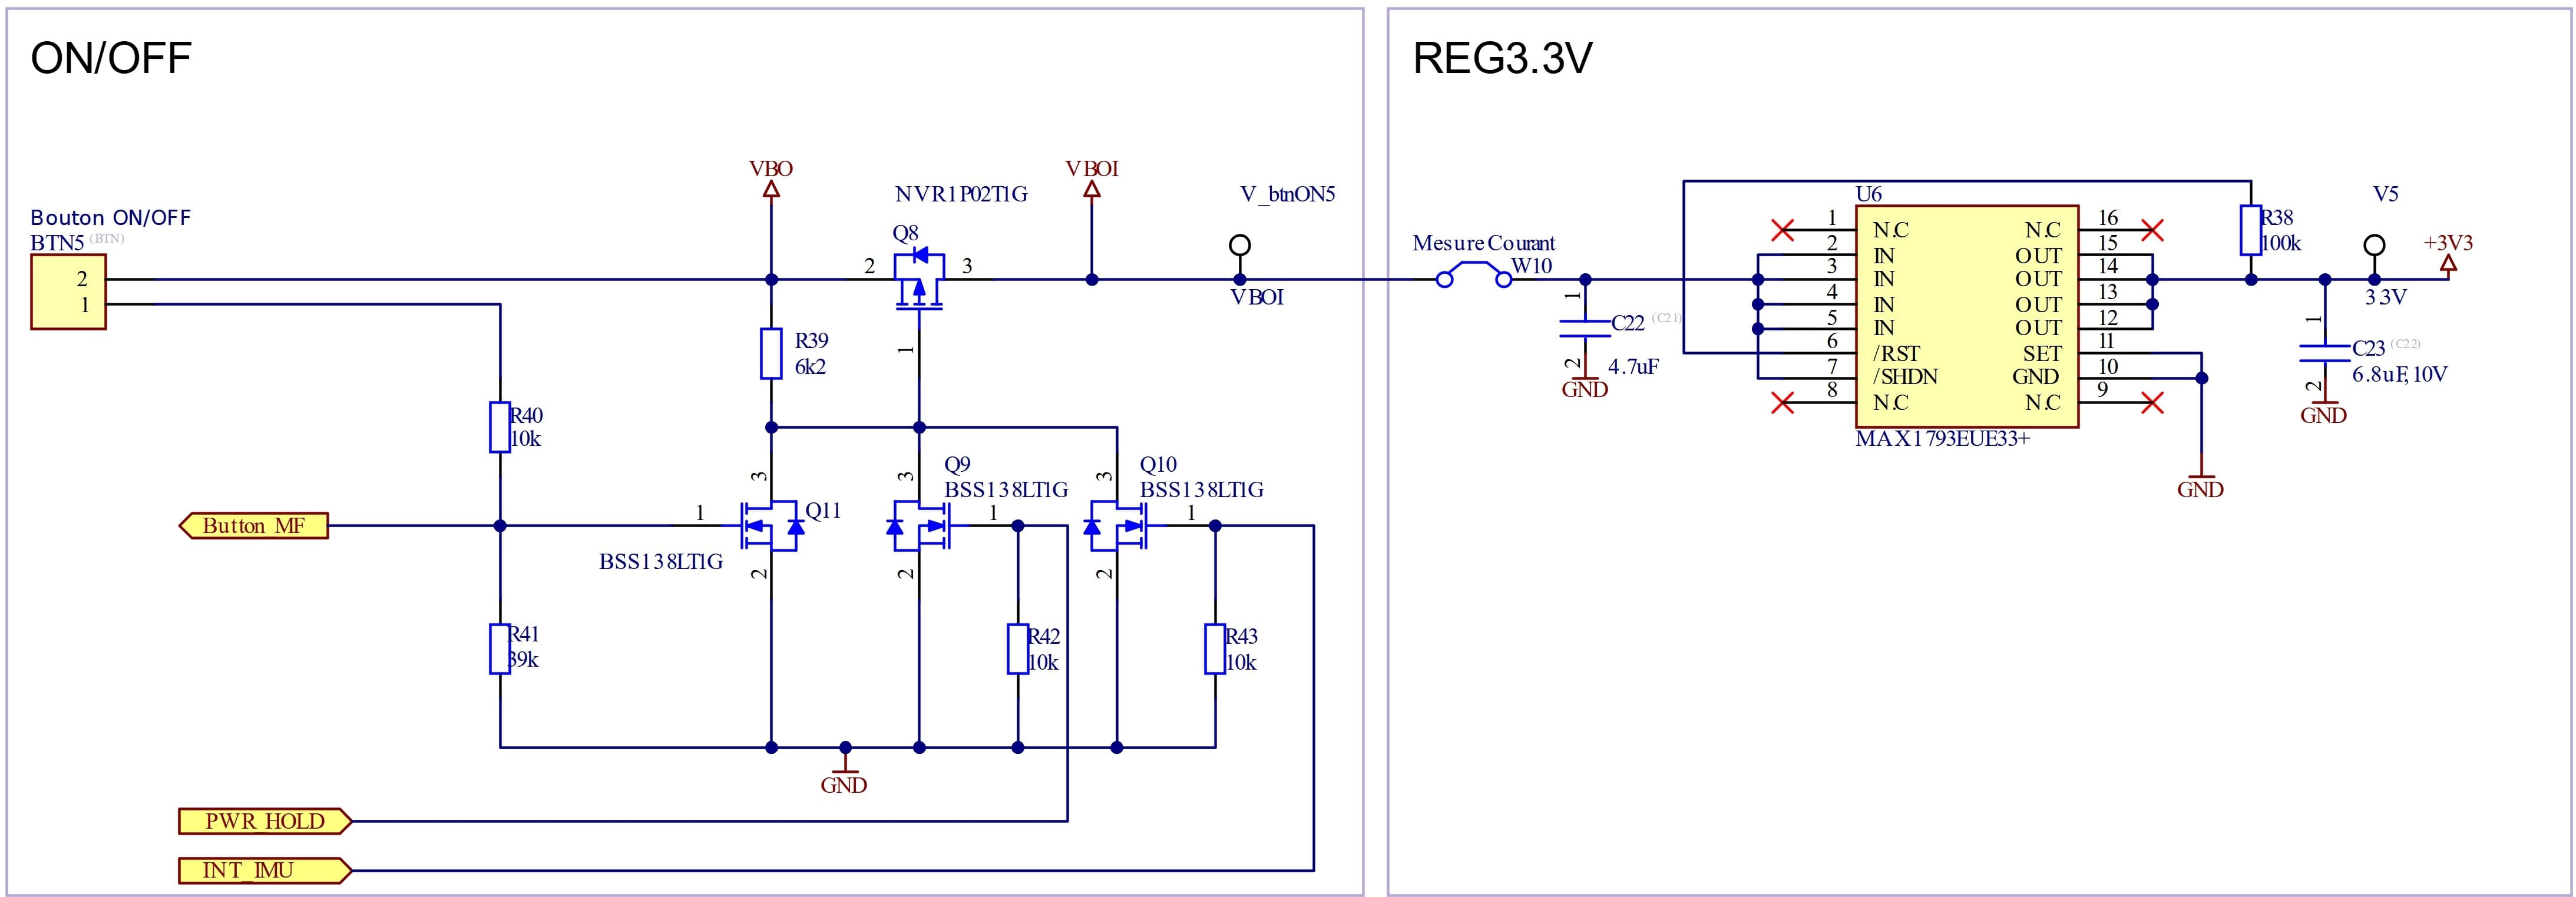
\includegraphics[width=1\linewidth]{../figures/etude/sch/ON-OFF}
	\caption{Schéma allumage du système.}
	\source{Auteur}
	\label{fig:on-off}
\end{figure}

Sur la figure \ref{fig:on-off}, nous observons les différentes manières de connecter la tension régulée de la batterie au régulateur linéaire \textbf{3.3V}. Quand cette connexion n'est pas réalisée, le système n'est pas alimenté, à l'exception de l'\gls{imu} qui peut être alimenté de manière autonome. Pour mettre en marche le système, trois options sont possibles : \vspace{2mm}

\begin{itemize}
	\item[\faChevronRight] Le microcontrôleur peut maintenir le système alimenté avec \textbf{PWR\_HOLD}. 
	\item[\faChevronRight] L'\gls{imu} peut 'allumer le système avec son interruption \textbf{INT\_IMU}. 
	\item[\faChevronRight] Un bouton peut être préssé pour enclencher la carte \textbf{Button\_MF}. 
\end{itemize}

\subsection{Conclusion et perspectives de l'étude} \label{ssec:Conclusion-etude}

Tout au long de cette étude, nous avons pu décomposer et analyser le processus de développement du schéma électronique. La démarche a priorisé la modularité, avec une division du système en trois blocs : \hyperref[ssec:Dev-MCU]{\textbf{Microcontrôleur \ref{ssec:Dev-MCU}}}, \hyperref[ssec:Dev-Devices]{\textbf{Périphériques \ref{ssec:Dev-Devices}}} et \hyperref[ssec:Dev-Alim]{\textbf{Alimentations \ref{ssec:Dev-Alim}}}. Cette approche a permis une meilleure lisibilité et une facilité d'adaptation quant au prototypage. Les différentes interactions et connexions entre les composants ont été détaillées.

Par la suite, le circuit imprimé sera développé, les composant placés et routés le tout dans un design petit et compact. La modularité du projet, permettra des tests empiriques sur les différents blocs du système, lors de la mise en service.




% ---------- DÉVELOPPEMENT PCB ----------------------------------
\section{Développement du circuit-imprimé} \label{sec:Dev-PCB}
Dans cette section, nous nous attarderons sur le processus de conception et de développement du \gls{pcb}. Nous aborderons également les différents aspects mécanique d'intégration du projet, en essayant d'analyser les différentes contraintes des composants et la structure globale. Cette analyse combinée des aspects électroniques et mécaniques est cruciale pour assurer la réussite du projet.

\clearpage

\subsection{Mécanique du projet} \label{ssec:mechProjet}
L'un des objectifs majeurs du projet est de concevoir un produit qui, par sa petite taille et son design compact, se prête à une installation qui se veut à la fois discrète et non encombrante.
 
\subsubsection{Choix du boitier}
Pour réduire la taille au maximum, un processus itératif a eu lieu, consistant à trouver un boîter plastique le plus petit possible et d'essayer en respectant les contraintes de taille, de placer les composants, puis, d'observer et déduire si la taille est suffisante. Grâce à cette procédure itérative, un boîtier a été déterminé : le \fbox{\textbf{SIC5-9-3B}} de chez \href{https://www.takachi-enclosure.com/products/SIC}{TAKACHI}.

\begin{figure}[h!]
	\centering
	\begin{subfigure}[b]{0.6\textwidth}
		\centering
		\includegraphics[width=\textwidth]{../figures/dev-pcb/boitier-dim}
		\caption{Dimensions boîtier}
		\label{fig:boitier-dim}
	\end{subfigure}
	\hfill
	\begin{subfigure}[b]{0.35\textwidth}
		\centering
		\includegraphics[width=\textwidth]{../figures/dev-pcb/boitier-dims-pcb}
		\caption{Dimension trous \gls{pcb}}
		\label{fig:boitier-dims-pcb}
	\end{subfigure}
	\caption{Dimensions du SIC5-9-3B.}
	\source{\href{https://www.takachi-enclosure.com/products/SIC}{\Gls{datasheet} du SIC5-9-3B, TAKACHI}}
	\label{fig:boitier-dimensions}
\end{figure}

\subsubsection{Placement des composants} \label{ssec:placementComp}
Désormais, sachant que nous connaissons les dimensions du \gls{pcb} grâce à la figure \ref{fig:boitier-dims-pcb}, nous pouvons positionner les composants de manière optimisée pour le routage et la mécanique. En prenant différents éléments en compte :

\begin{table}[!h]
\begin{adjustbox}{max width=\textwidth}
	\begin{tabular}{llll}
	\hline
	& Élément & & Contraintes, règles et dispositions particulières \\
	\hline
	\faChevronRight & \textbf{Connecteur USB} & : & Placer proche du bord, usinage du boitier pour passer chargeur. \\
	\faChevronRight & \textbf{Connecteur \micro SD} & : & Proche du bord, facile d'accès. \\
	\faChevronRight & \textbf{\gls{gnss}} & : & Isolé des autres composants, faciliter réception. \\
	\faChevronRight & \textbf{Carte BNO055} & : & Espace requis, permettre de le braser sur le \gls{pcb}. \\
	\faChevronRight & \textbf{LED de vie} & : & Dégagée, peut être déportée avec un guide-lumière. \\
	\faChevronRight & \textbf{Connecteur batterie} & : & Accessible et permettre de passer les fils de l'autre coté du \gls{pcb}. \\
	\faChevronRight & \textbf{Connecteur bouton ON/OFF} & : & Bouton déporté sur le boîtier. \\
	\faChevronRight & \textbf{Bouton reset} & : & Accessible pendant le développement et en cas de bug. \\
	\end{tabular}	
\end{adjustbox}
\caption{Tableau des contraintes de placement.}
\label{tab:reglesPlacement}
\source{Auteur}
\end{table}

\clearpage

\begin{figure}[h]
	\centering
	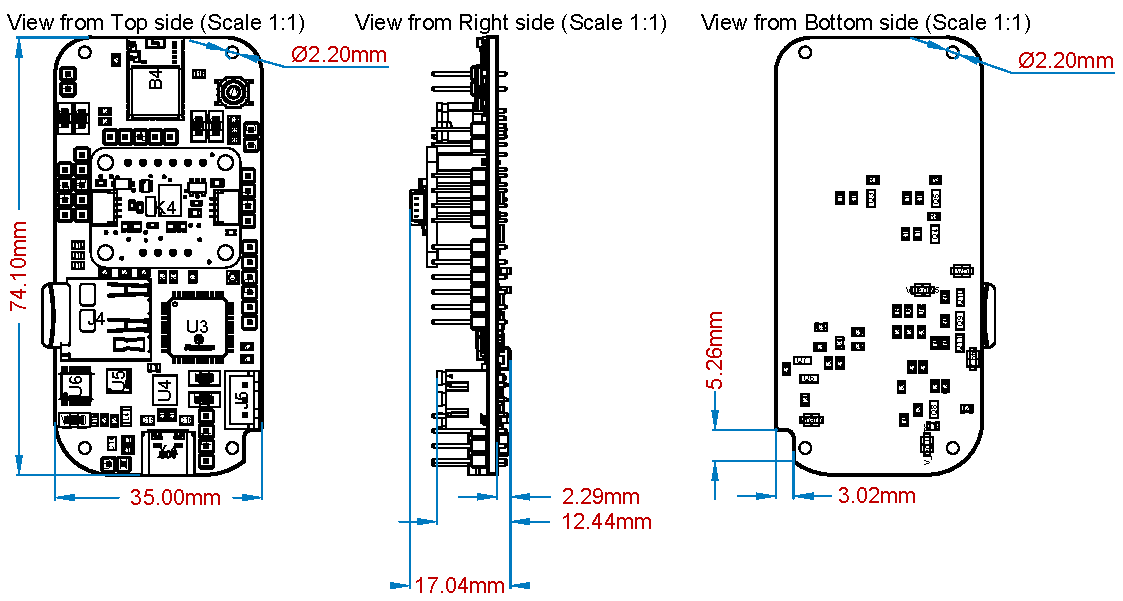
\includegraphics[width=.83\linewidth]{../figures/dev-pcb/PCB-Dims}
	\caption{Placement des composant et dimensions de la carte.}
	\source{Auteur}
	\label{fig:pcb-dims}
\end{figure}

En considérant les contraintes des différents éléments de la table \ref{tab:reglesPlacement}, nous obtenons un design tel que celui de la figure \ref{fig:pcb-dims}. Nous y observons plusieurs solutions apportées telles que :
un trou (En bas à droite du \gls{pcb}) permettant de passer les fils de la batterie, une carte SD et un connecteur USB placés proche du bord, un bouton de reset accessible et un \gls{gnss} isolé du reste pour garantir l'intégrité de l'antenne. 

\subsubsection{Assemblage}
Lors de cette section, nous allons assembler le circuit imprimé avec ses composants et la batterie, dans le modèle 3D du boîtier \textbf{SIC5-9-3B}.

\begin{figure}[!h]
	\centering
	\begin{subfigure}[b]{0.24\textwidth}
		\centering
		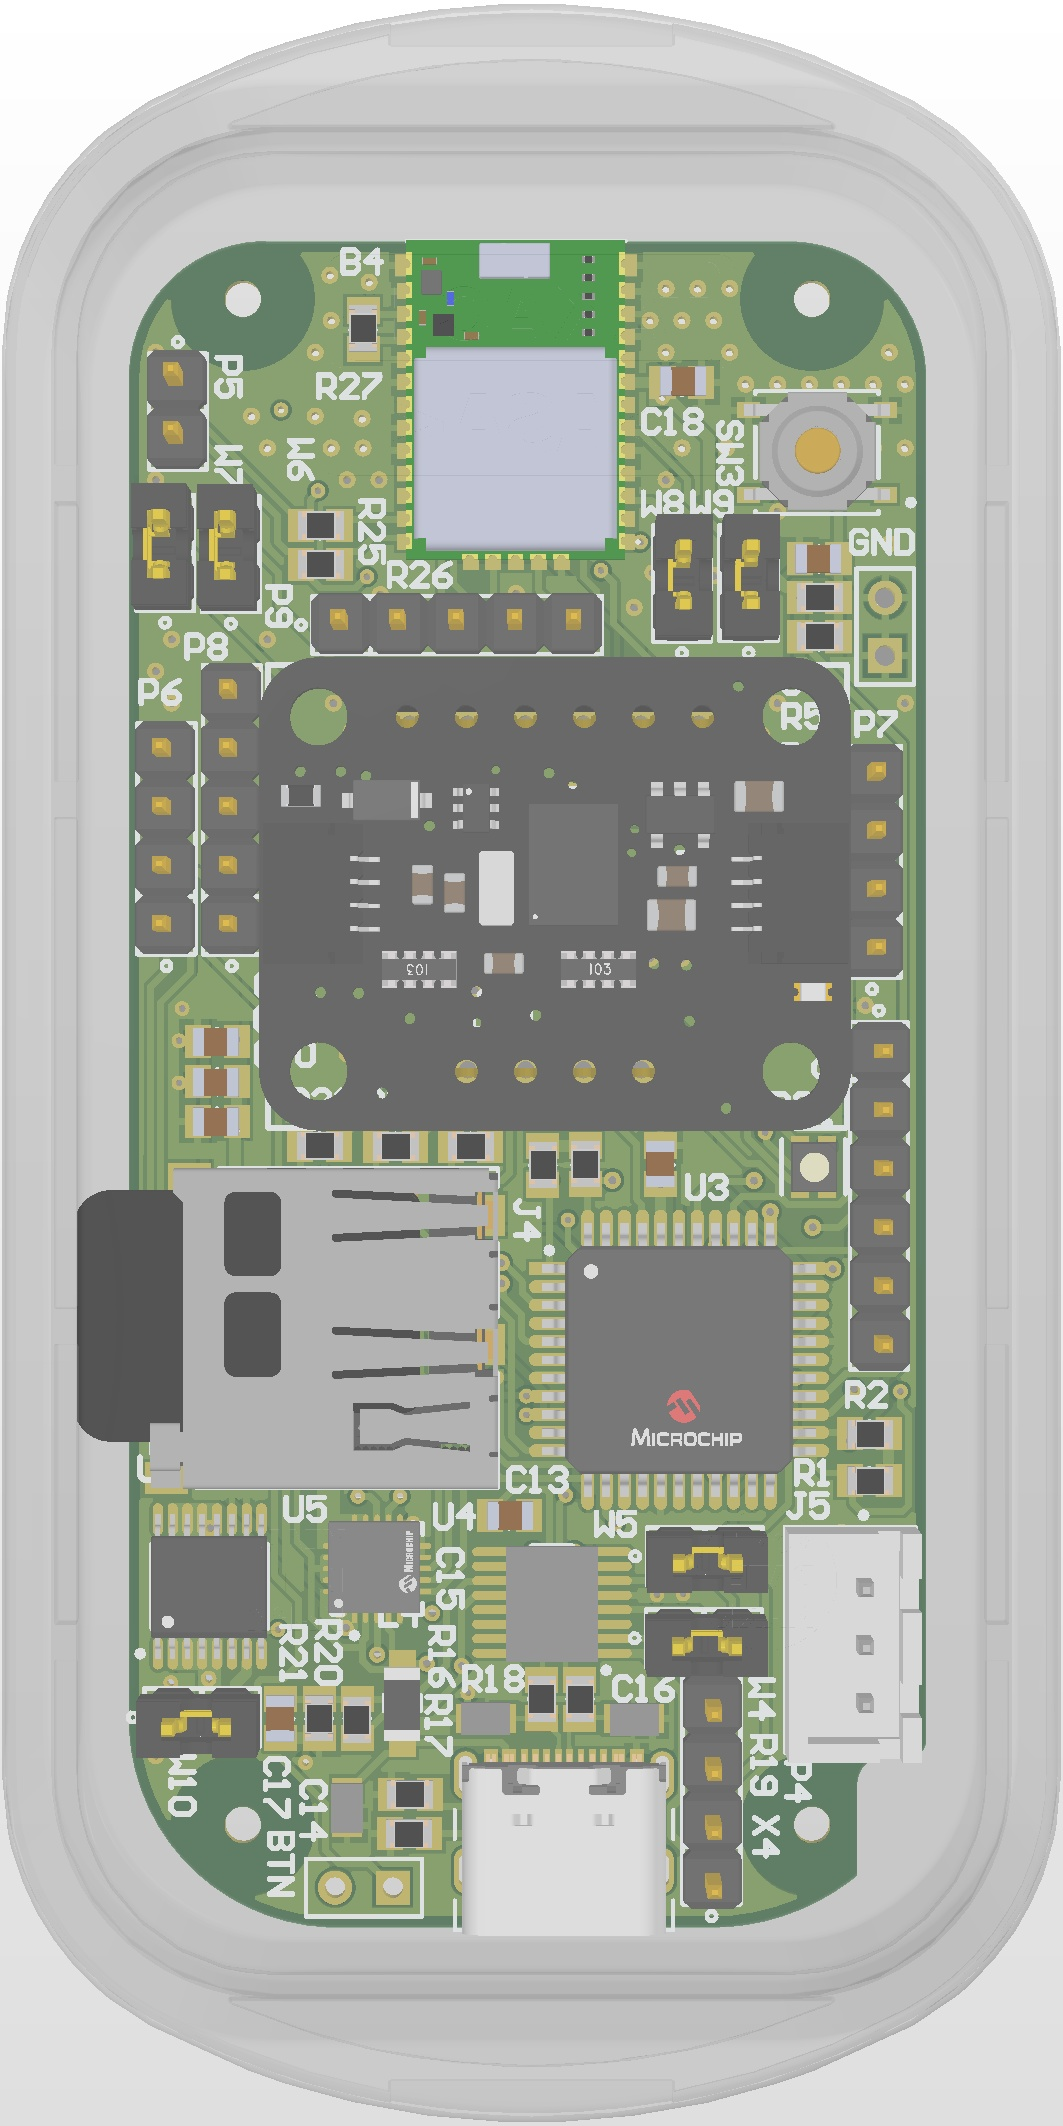
\includegraphics[width=\textwidth]{../figures/dev-pcb/3d-view3}
		\caption{Vue 3D, 1}
		\label{fig:3d-1}
	\end{subfigure}
	\hfill
	\begin{subfigure}[b]{0.33\textwidth}
		\centering
		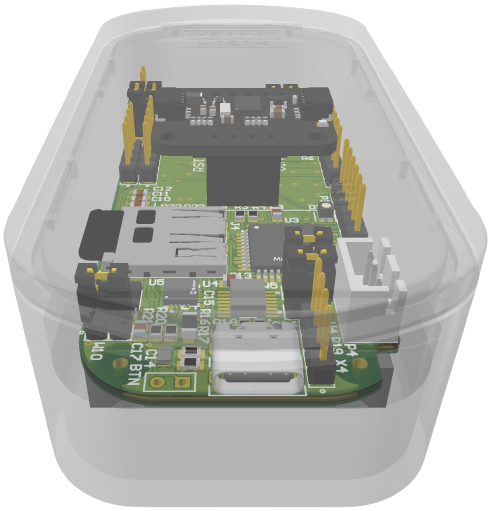
\includegraphics[width=\textwidth]{../figures/dev-pcb/3d-view2}
		\caption{Vue 3D, 2}
		\label{fig:3d-2}
	\end{subfigure}
	\hfill
	\begin{subfigure}[b]{0.36\textwidth}
		\centering
		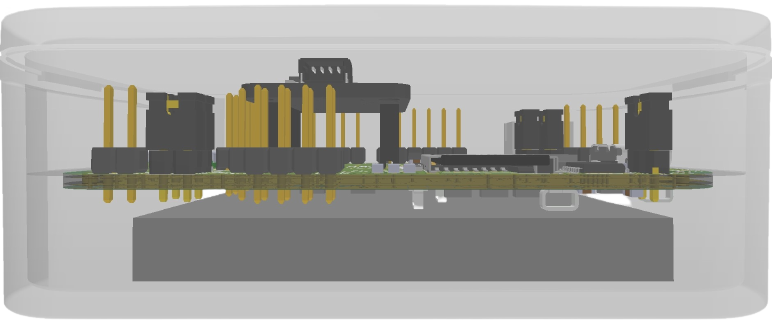
\includegraphics[width=\textwidth]{../figures/dev-pcb/3d-view1}
		\caption{Vue 3D, 3}
		\label{fig:3d-3}
	\end{subfigure}
	\caption{Vues 3d de l'assemblage.}
	\label{fig:MechAssembly}
	\source{Auteur}
\end{figure}

Comme nous pouvons observer sur la figure \ref{fig:MechAssembly}, l'ensemble, s'assemble correctement.

\clearpage

\subsection{Bill of materials} \label{ssec:BOM}
Avec le schéma électronique et la mécanique désormais finalisés, nous pouvons dresser une liste des composants nécessaires. La table \ref{tab:BOM_PRIX} répertorie les composants \textbf{hors-stock} qui ont été commandés auprès de différents fournisseurs. La table \ref{tab:BOM-Stock}, quant à elle, liste les composants \textbf{en stock} disponibles dans les locaux de l'école supérieure, avec leurs coûts respectifs. Il est à noter que ces derniers n'ont pas été commandés. Les tableaux \ref{tab:Bom_resistors} et \ref{tab:Bom_Capa} détaillent respectivement les valeurs des résistances et des condensateurs utilisés pour le projet.

\begin{table}[h]
	\centering
	\resizebox{\textwidth}{!}{%
		\begin{tabular}{|l|llll|}
			\hline
			Composant                            & \multicolumn{1}{l|}{Fournisseur} & \multicolumn{1}{l|}{Réference}              & \multicolumn{1}{l|}{Quantité} & Prix [CHF] \\ \hline
			Batterie PICPAL36                    & \multicolumn{1}{l|}{Farnell}     & \multicolumn{1}{l|}{PICPAL36}               & \multicolumn{1}{l|}{1}        & 36,54      \\ \hline
			BNO055-Adafruit                      & \multicolumn{1}{l|}{Digikey}     & \multicolumn{1}{l|}{1528-4646-ND}           & \multicolumn{1}{l|}{1}        & 26,06      \\ \hline
			GNSS                                 & \multicolumn{1}{l|}{Digikey}     & \multicolumn{1}{l|}{672-CAM-M8C-0CT-ND}     & \multicolumn{1}{l|}{1}        & 23,49      \\ \hline
			Boitier boite noire                  & \multicolumn{1}{l|}{Farnell}     & \multicolumn{1}{l|}{CHH9840BK}              & \multicolumn{1}{l|}{1}        & 6,84       \\ \hline
			Guide lumière &
			\multicolumn{1}{l|}{Digikey} &
			\multicolumn{1}{l|}{\begin{tabular}[c]{@{}l@{}}LFB075CTP-ND\\ 492-1980-ND\end{tabular}} &
			\multicolumn{1}{l|}{4} &
			6,13 \\ \hline
			PIC32MX274F256D &
			\multicolumn{1}{l|}{Digikey} &
			\multicolumn{1}{l|}{PIC32MX274F256DT-I/PTCT-ND} &
			\multicolumn{1}{l|}{1} &
			6,07 \\ \hline
			Bouton poussoir ext.                 & \multicolumn{1}{l|}{Digikey}     & \multicolumn{1}{l|}{EG5949-ND}              & \multicolumn{1}{l|}{1}        & 4,54       \\ \hline
			Connecteur uSD                       & \multicolumn{1}{l|}{Digikey}     & \multicolumn{1}{l|}{732-3819-1-ND}          & \multicolumn{1}{l|}{1}        & 2,71       \\ \hline
			LEDS &
			\multicolumn{1}{l|}{Digikey} &
			\multicolumn{1}{l|}{\begin{tabular}[c]{@{}l@{}}516-3906-1-ND\\ 732-4985-1-ND\end{tabular}} &
			\multicolumn{1}{l|}{4} &
			2,05 \\ \hline
			Connecteur USB                       & \multicolumn{1}{l|}{Digikey}     & \multicolumn{1}{l|}{2073-USB4105-GF-ACT-ND} & \multicolumn{1}{l|}{1}        & 1,97       \\ \hline
			Mosfet P                             & \multicolumn{1}{l|}{Digikey}     & \multicolumn{1}{l|}{NVR1P02T1GOSCT-ND}      & \multicolumn{1}{l|}{2}        & 0,7        \\ \hline
			Bouton tactile reset                 & \multicolumn{1}{l|}{Digikey}     & \multicolumn{1}{l|}{CKN12221-1-ND}          & \multicolumn{1}{l|}{1}        & 0,35       \\ \hline
			Ferrite Bead 600 Ohm                 & \multicolumn{1}{l|}{Digikey}     & \multicolumn{1}{l|}{732-4655-1-ND}          & \multicolumn{1}{l|}{1}        & 0,22       \\ \hline
			Connecteur batterie                  & \multicolumn{1}{l|}{Farnell}     & \multicolumn{1}{l|}{B3B-XH-A (LF)(SN)}      & \multicolumn{1}{l|}{1}        & 0,11       \\ \hline
			\multicolumn{1}{|c|}{\textbf{TOTAL}} & \multicolumn{4}{c|}{\textbf{117.78}}                                                                                        \\ \hline
		\end{tabular}%
	}
	\caption{Liste des composants hors-stocks.}
	\label{tab:BOM_PRIX}
\end{table}

\vspace{-7mm}

\begin{table}[h]
	\centering
	\resizebox{\textwidth}{!}{%
		\begin{tabular}{|l|llll|}
			\hline
			Composant                       & \multicolumn{1}{l|}{Fournisseur} & \multicolumn{1}{l|}{Réference}              & \multicolumn{1}{l|}{Quantité} & Prix [CHF] \\ \hline
			Régulateur linéaire 3.3V        & \multicolumn{1}{l|}{Digikey}     & \multicolumn{1}{l|}{MAX1793EUE33+-ND}       & \multicolumn{1}{l|}{1}        & 3.85       \\ \hline
			IC chargeur de batterie lithium & \multicolumn{1}{l|}{Digikey}     & \multicolumn{1}{l|}{MCP73871T-2CCI/MLCT-ND} & \multicolumn{1}{l|}{1}        & 2.1        \\ \hline
			Mosfet Canal N                       & \multicolumn{1}{l|}{Digikey} & \multicolumn{1}{l|}{BSS138LCT-ND}  & \multicolumn{1}{l|}{7} & 2.1  \\ \hline
			FTDI, USB-UART                       & \multicolumn{1}{l|}{Digikey} & \multicolumn{1}{l|}{768-1154-5-ND} & \multicolumn{1}{l|}{1} & 1.97 \\ \hline
			\multicolumn{1}{|c|}{\textbf{TOTAL}} & \multicolumn{4}{c|}{\textbf{10.02}}                                                               \\ \hline
		\end{tabular}%
	}
	\caption{Liste des composants en stock.}
	\label{tab:BOM-Stock}
\end{table}

\vspace{-7mm}

\begin{table}[h!]
	\centering
	\resizebox{\textwidth}{!}{%
		\begin{tabular}{|lcccccccccccccc|}
			\hline
			\multicolumn{15}{|c|}{\textbf{Résistances}} \\ \hline
			\multicolumn{1}{|l|}{Valeur} &
			\multicolumn{1}{c|}{27R} &
			\multicolumn{1}{c|}{220R} &
			\multicolumn{1}{c|}{270R} &
			\multicolumn{1}{c|}{430R} &
			\multicolumn{1}{c|}{1k} &
			\multicolumn{1}{c|}{5k1} &
			\multicolumn{1}{c|}{6k2} &
			\multicolumn{1}{c|}{8k2} &
			\multicolumn{1}{c|}{10k} &
			\multicolumn{1}{c|}{15k} &
			\multicolumn{1}{c|}{39k} &
			\multicolumn{1}{c|}{47k} &
			\multicolumn{1}{c|}{51k} &
			100k \\ \hline
			\multicolumn{1}{|l|}{Quantitée} &
			\multicolumn{1}{c|}{2} &
			\multicolumn{1}{c|}{3} &
			\multicolumn{1}{c|}{4} &
			\multicolumn{1}{c|}{6} &
			\multicolumn{1}{c|}{1} &
			\multicolumn{1}{c|}{2} &
			\multicolumn{1}{c|}{1} &
			\multicolumn{1}{c|}{1} &
			\multicolumn{1}{c|}{12} &
			\multicolumn{1}{c|}{2} &
			\multicolumn{1}{c|}{4} &
			\multicolumn{1}{c|}{1} &
			\multicolumn{1}{c|}{4} &
			1 \\ \hline
		\end{tabular}%
	}
	\caption{Liste des valeurs des résistances.}
	\label{tab:Bom_resistors}
\end{table}

\vspace{-7mm}

\begin{table}[h!]
	\centering
	\begin{tabular}{|lcccccc|}
		\hline
		\multicolumn{7}{|c|}{\textbf{Condensateurs}} \\ \hline
		\multicolumn{1}{|l|}{Valeur} &
		\multicolumn{1}{c|}{47pF} &
		\multicolumn{1}{c|}{10nF} &
		\multicolumn{1}{c|}{100nF} &
		\multicolumn{1}{c|}{4.7uF} &
		\multicolumn{1}{c|}{6.8uF} &
		10uF \\ \hline
		\multicolumn{1}{|l|}{Quantitée} &
		\multicolumn{1}{c|}{2} &
		\multicolumn{1}{c|}{2} &
		\multicolumn{1}{c|}{7} &
		\multicolumn{1}{c|}{4} &
		\multicolumn{1}{c|}{1} &
		2 \\ \hline
	\end{tabular}
	\caption{Liste des valeurs des condensateurs.}
	\label{tab:Bom_Capa}
\end{table}

\clearpage

\subsection{Routage} \label{ssec:routage}
Une fois les composants placés, les pistes et les plan ont put être 

\begin{figure}[!h]
	\centering
	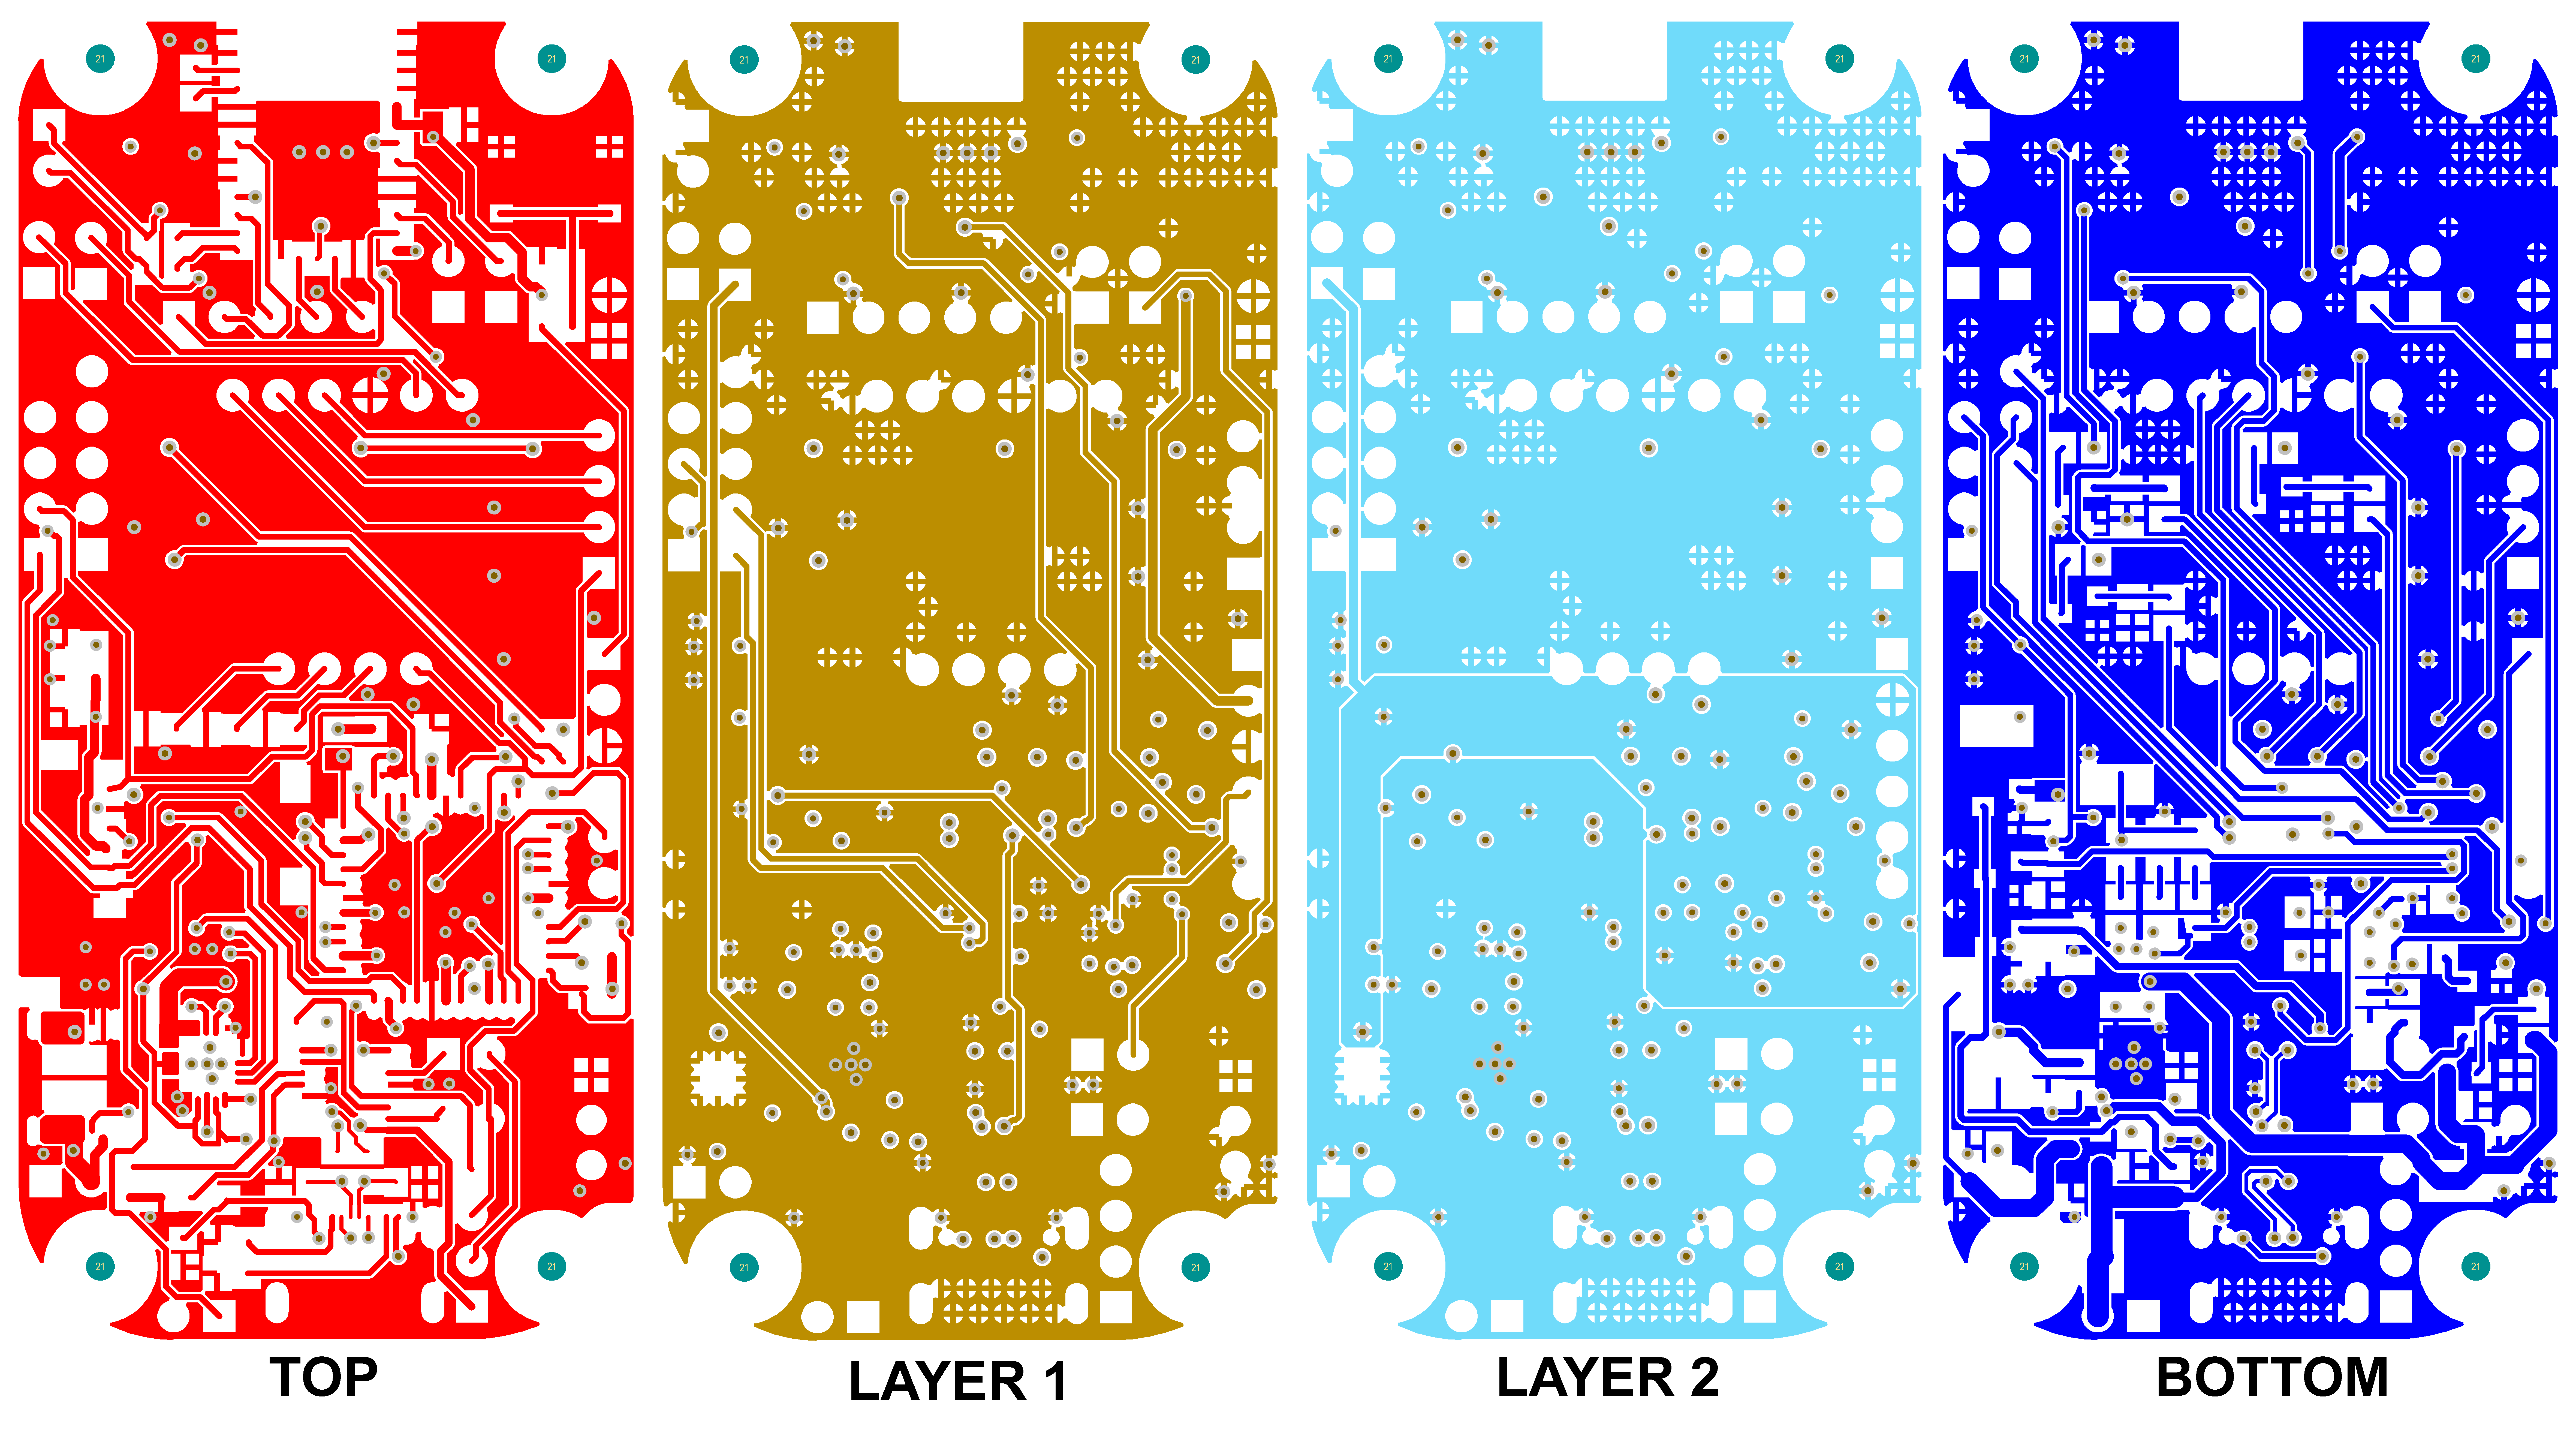
\includegraphics[width=.9\linewidth]{../figures/dev-pcb/Couches-layout}
	\caption{Routage des différentes couches.}
	\label{fig:couches-layout}
	\source{Auteur}
\end{figure}

Les justifications du routage des différentes couche sont présentées dans la table \ref{tab:descr-routage}.

\begin{table}[!h]
	\centering
	\resizebox{.63\textwidth}{!}{%
		\begin{tabular}{|lll|}
			\hline
			\textbf{TOP}     &                 &                                  \\
			& \faChevronRight & Composants à braser au four.     \\
			& \faChevronRight & Signaux proches du \gls{mcu}.     \\
			& \faChevronRight & Signaux sortant du \gls{gnss}.   \\
			& \faChevronRight & Pistes horizontales.             \\
			& \faChevronRight & Plan de masse.                    \\
			& \faChevronRight & Connecteurs pour boutons et batterie. \\ \hline
			\textbf{LAYER 1} &                 &                                  \\
			& \faChevronRight & Pistes de signaux verticaux.     \\
			& \faChevronRight & Plan de masse.                   \\ \hline
			\textbf{LAYER 2} &                 &                                  \\
			& \faChevronRight & Plan de masse homogène.          \\
			& \faChevronRight & Plan de 3.3V.                    \\ \hline
			\textbf{BOTTOM}  &                 &                                  \\
			& \faChevronRight & Composants des régulateurs.      \\
			& \faChevronRight & Mosfets et composants passifs.   \\
			& \faChevronRight & Pistes de signaux verticaux.     \\
			& \faChevronRight & Plan de masse.                   \\ \hline
		\end{tabular}%
	}
	\caption{Description des éléments du routage.}
	\label{tab:descr-routage}
\end{table}

Le routage étant complété et contrôlé, il a pu être commandé sous forme de panel avec un pochoir chez \href{https://www.eurocircuits.com/}{\textit{Eurocircuit}}. Celui-ci a eu des retards de production et de livraison par UPS.

\clearpage

\subsection{Conclusion et perspectives de la conception}

Durant cette section, nous avons conçu le circuit imprimé de la boîte noire, défini son implémentation dans un petit boîtier plastique, vérifié l'intégration du circuit et de la batterie à l'intérieur, et avons décrit les différentes justifications de développement. Par la suite, la carte sera montée, brasée, et les phases de programmation sur la carte auront lieu.




% ---------- DÉVELOPPEMENT SOFTWARE ----------------------------- 
\section{Développement du firmware} \label{sec:Dev-firmware}

Lors de cette section, nous décrirons le processus de développement du firmware du PIC32. Les décisions prises seront expliquées et les différents algorithmes seront illustrés et décrits.

En premier lieux nous allons analyser lors de la section \ref{ssec:ProtocolGNSS} comment traiter les données du \gls{gnss}, il s'agit d'un élément critique.


\subsection{Protocoles du GNSS} \label{ssec:ProtocolGNSS}
Il existe différents protocoles pour le format de données de localisation. Le \textbf{CAM-M8C-0} supporte plusieurs protocoles, visibles sur la figure \ref{fig:protocolsGNSS} :

\begin{figure}[h]
	\centering
	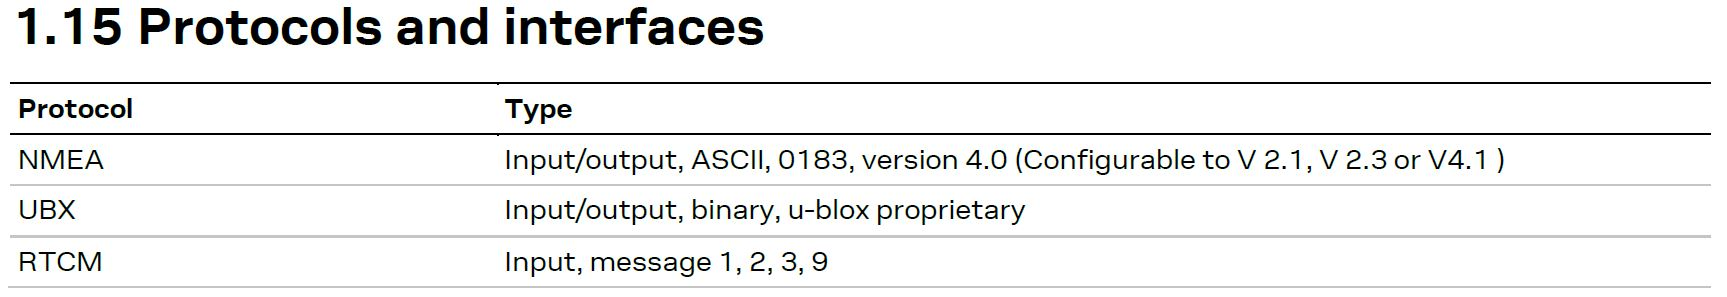
\includegraphics[width=.75\linewidth]{../figures/code/Protocols}
	\caption{Protocoles disponibles.}
	\source{\Gls{datasheet} du \href{https://content.u-blox.com/sites/default/files/CAM-M8-FW3\_DataSheet\_\%28UBX-15031574\%29.pdf}{CAM-M8C-0}}
	\label{fig:protocolsGNSS}
\end{figure} \vspace{-4mm}

\begin{tabularx}{\textwidth}{llX}
	\textbf{NMEA}& : & Norme établie par la \textit{National Marine Electronics Association}. Elle suit un format \fbox{\textbf{ASCII}}. \\
	\textbf{UBX} & : & Format propriétaire de u-blox avec des données \fbox{\textbf{binaires}}. Il permet d'envoyer des trames de configuration. \\
	\textbf{RTCM} & : & Protocole pour des données GPS différentielles. Établi par la \textit{Radio Technical Commission for Maritime Service}.
\end{tabularx} 


Le \textbf{CAM-M8C-0} est configuré, par défaut, pour envoyer des messages au format NMEA, comme illustré sur la figure \ref{fig:default-messages}. \vspace{+2mm}

\begin{figure}[!h]
	\centering
	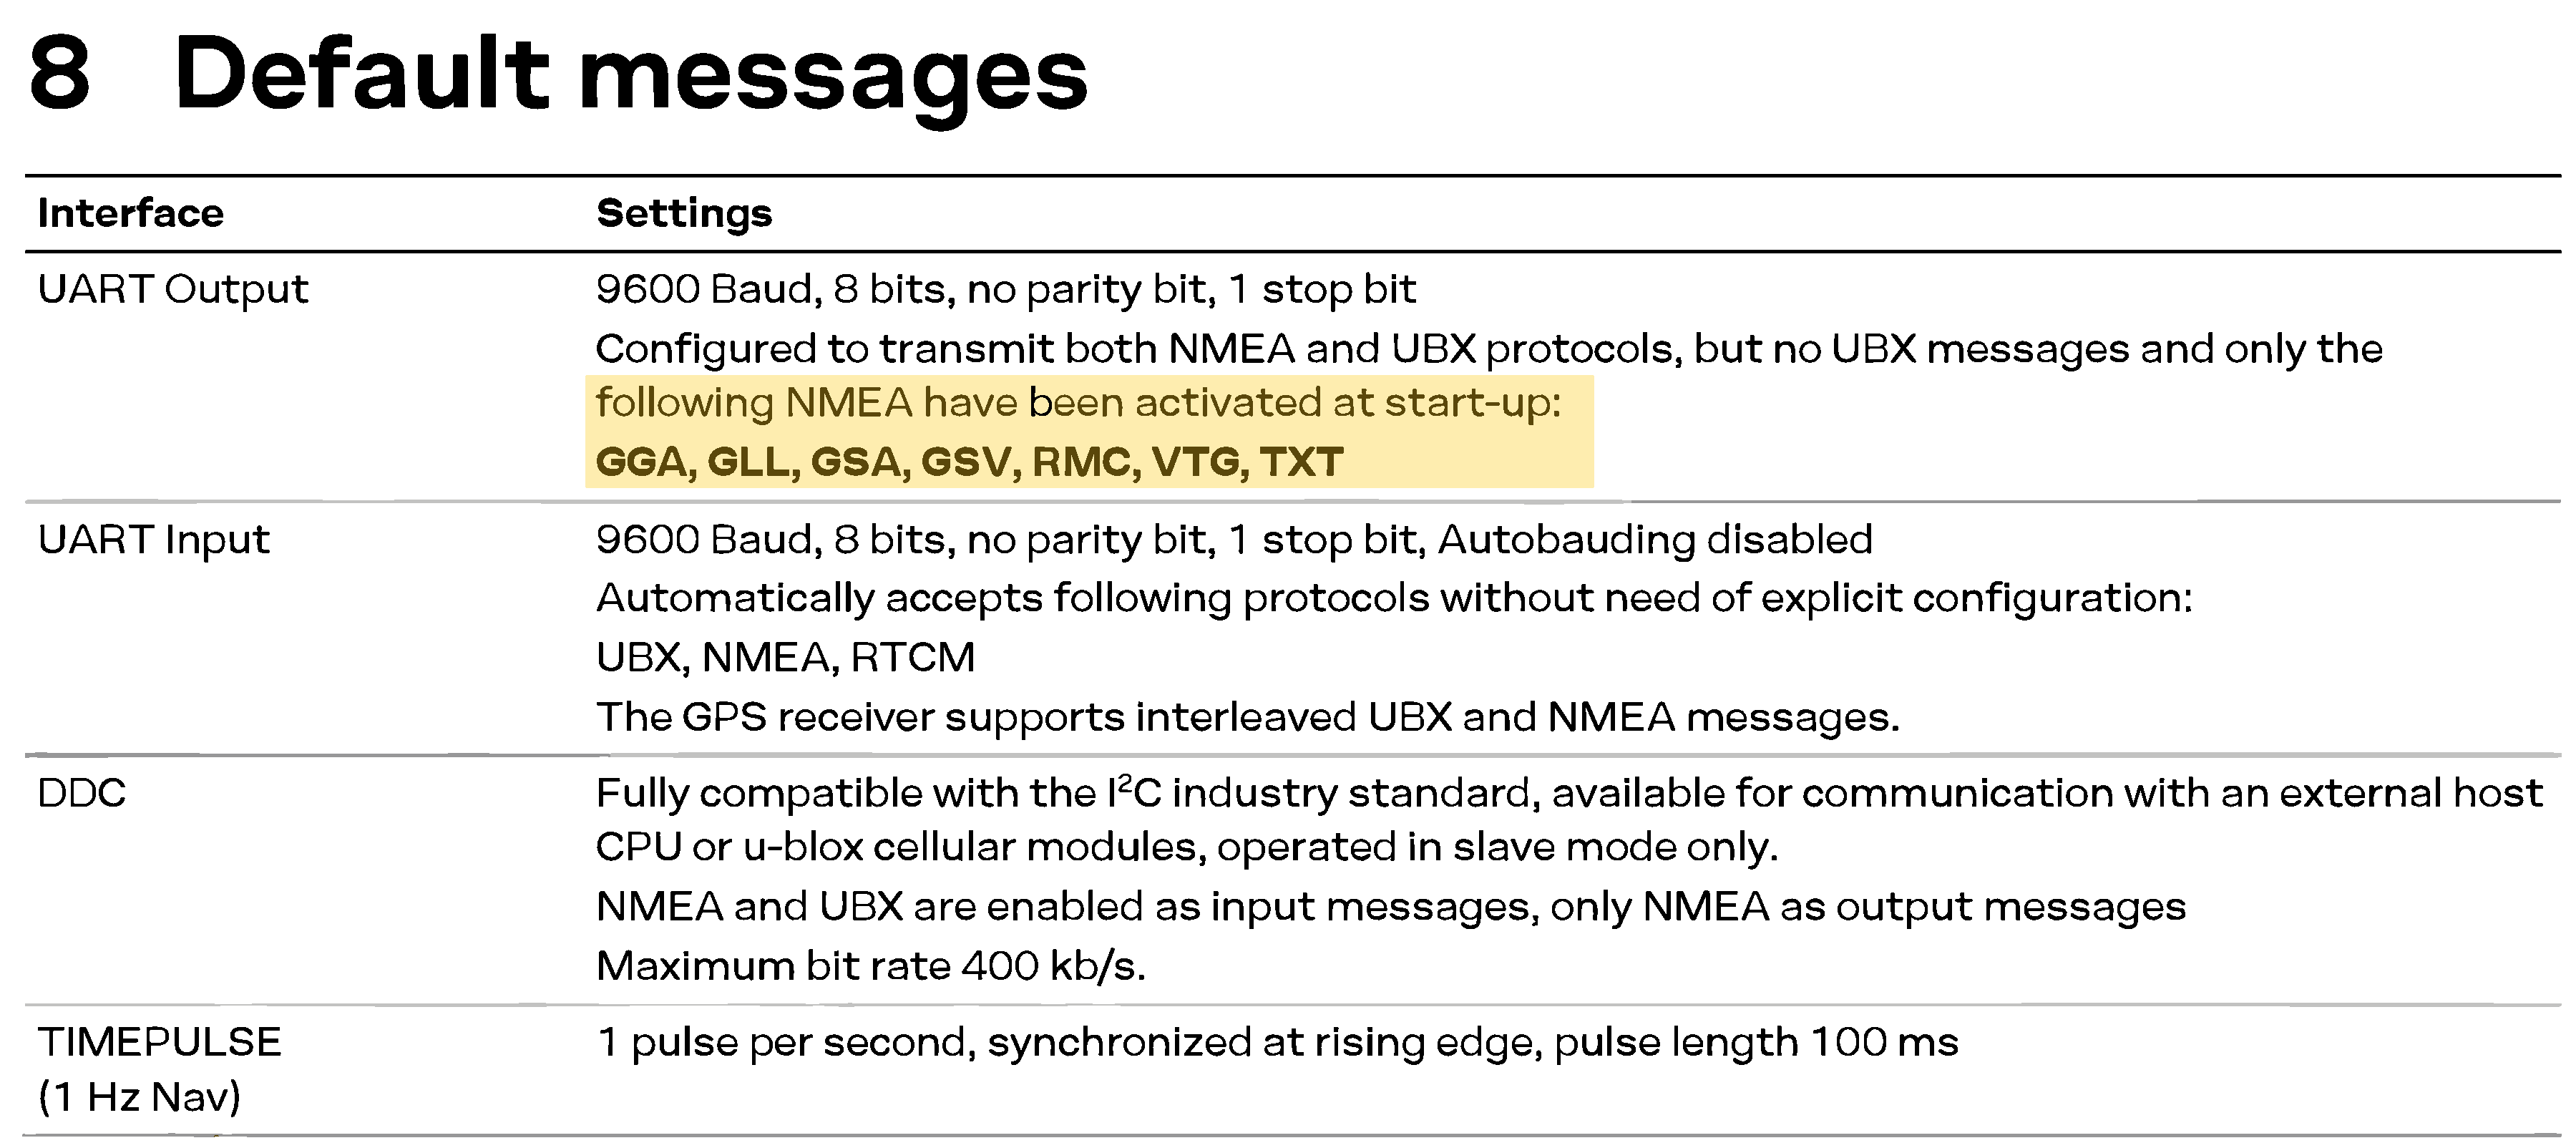
\includegraphics[width=0.7\linewidth]{../figures/code/Default-messages}
	\caption{Protocole par défaut.}
	\source{\Gls{datasheet} du \href{https://content.u-blox.com/sites/default/files/CAM-M8-FW3\_DataSheet\_\%28UBX-15031574\%29.pdf}{CAM-M8C-0}}
	\label{fig:default-messages}
\end{figure}

\clearpage

\subsubsection{Messages NMEA}
Comme nous avons pu constater sur la figure \ref{fig:default-messages}, il y a plusieurs messages \textbf{NMEA} : 

\textbf{GGA, GLL, GSA, GSV, RMC, VTG, TXT}

Ceux-ci sont décris dans le \href{https://www.ekf.de/c/cgps/cg2/inf/nmea_reference_manual.pdf}{manuel de référence du protocole NMEA} sur la figure \ref{fig:messages-nmea}

\begin{figure}[h]
	\centering
	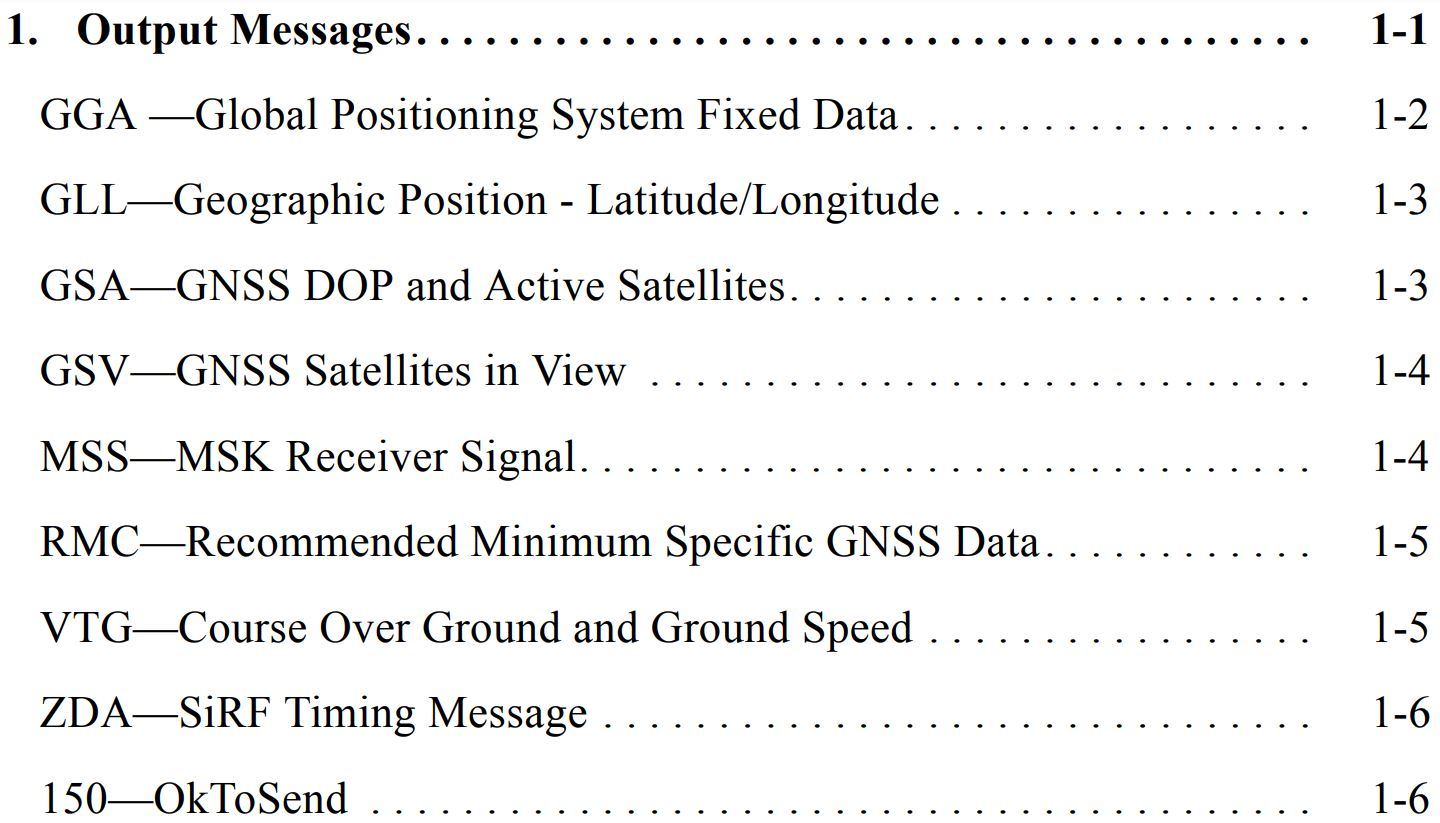
\includegraphics[width=0.55\linewidth]{../figures/code/Messages-NMEA}
	\caption{Messages NMEA.}
	\source{\href{https://www.ekf.de/c/cgps/cg2/inf/nmea_reference_manual.pdf}{Manuel du protocole NMEA}}
	\label{fig:messages-nmea}
\end{figure}

Les différents messages de la figure \ref{fig:messages-nmea} présentent des différentes données sous divers formats. Les messages peuvent être activés ou désactivés en configurant le module u-blox.

\subsubsection{Interprétation des données NMEA}
Avant d'avoir le \gls{pcb} monté et exploitable, sachant que nous connaissons le protocole par défaut du module, nous pouvons analyser des données \textbf{NMEA} pour mieux les comprendre et les traiter par la suite. Pour ce faire, le site \href{https://www.nmeagen.org/}{https://www.nmeagen.org/} permet de générer des coordonnées avec le protocole \textbf{NMEA}.

\begin{figure}[h]
	\centering
	\includegraphics[width=.75\textwidth]{../figures/code/map-localisation}
	\caption{Application d'une localisation NMEA.}
	\source{\href{https://www.nmeagen.org/}{nmeagen.org}, aéroport de La Blécherette, Lausanne}
	\label{fig:map-localisation}
\end{figure}

Sur la figure \ref{fig:parsed-nmea}, les messages de la figure \ref{fig:map-localisation} sont décodés via un \href{https://swairlearn.bluecover.pt/nmea_analyser}{analyseur NMEA en ligne}.

\begin{figure}[h]
	\centering
	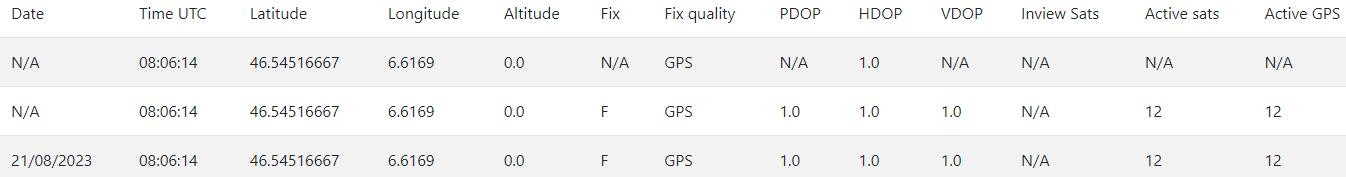
\includegraphics[width=0.8\linewidth]{../figures/code/parsed-nmea}
	\caption{Messages NMEA décodés.}
	\source{\href{https://swairlearn.bluecover.pt/nmea_analyser}{NMEA online analyser}}
	\label{fig:parsed-nmea}
\end{figure}

\clearpage

\subsubsection{Code décodeur de trame NMEA}
Afin de développer le code du décodeur \textbf{NMEA}, la librairie \href{https://github.com/kosma/minmea}{\textbf{minmea}} de licence libre, a pu être utilisée, modifiée et adaptée. Un algorithme a ensuite été mis en place :

\begin{itemize}
	\item[\oldstylenums{1}] Lecture du type de message (\textbf{GBS, GGA, GLL, GSA, GST, GSV, RMC, VTG, ZDA});
	\item[\oldstylenums{2}] Parsing des valeurs correspondantes à l'ID du message;
	\item[\oldstylenums{3}] Sauvegarde des valeurs dans une structure.
\end{itemize}


\begin{code}
\caption{gnss\_posGet\_nmea(...), décodage \textbf{NMEA}.}
\label{code:posget-nmea}
\begin{minted}[breaklines]{c}
// Get message ID, strict
*msg_id = minmea_sentence_id(message, true);
// Parse message depending on ID
if (*msg_id == MINMEA_SENTENCE_GBS)
	minmea_parse_gbs(&sentences->gbs, message);
else if (*msg_id == MINMEA_SENTENCE_GGA)
	minmea_parse_gga(&sentences->gga, message);
else if ...
\end{minted}
\end{code}

Dans le code \ref{code:posget-nmea}, on fait appel à une fonction qui va masquer les caractères du type du message. Ensuite, selon le message dont il s'agit, on le décode de différentes façons.

\begin{code}
\caption{minmea\_parse\_gbs(...), décodage message \textbf{GBS}.}
\label{code:parse-gbs}
\begin{minted}[breaklines]{c}
bool minmea_parse_gbs(struct minmea_sentence_gbs *frame, const char *sentence)
{
	// $GNGBS,170556.00,3.0,2.9,8.3,,,,*5C
	char type[6];
	if (!minmea_scan(sentence, "tTfffifff",
			type,
			&frame->time,
			&frame->err_latitude,
			&frame->err_longitude,
			&frame->err_altitude,
			&frame->svid,
			&frame->prob,
			&frame->bias,
			&frame->stddev
			))
		return false;
	if (strcmp(type+2, "GBS"))
		return false;
	return true;
}

\end{minted}
\end{code}

Dans le code \ref{code:parse-gbs}, on masque les éléments du message selon son format, d'une manière similaire à la fonction standard \textit{\textbf{scanf(...)}}.

\clearpage

Les données spécifique au message \textbf{GBS} sont ensuite stockées dans une structure, que l'on peut observer dans le code \ref{code:struct-gbs}.

\begin{code}
\caption{Structure \textbf{GBS}.}
\label{code:struct-gbs}
\begin{minted}[breaklines]{c}
struct minmea_sentence_gbs {
	struct minmea_time time;
	struct minmea_float err_latitude;
	struct minmea_float err_longitude;
	struct minmea_float err_altitude;
	int svid;
	struct minmea_float prob;
	struct minmea_float bias;
	struct minmea_float stddev;
};
\end{minted}
\end{code}

Sachant que plusieurs types de messages peuvent être interceptés, chacune des structures des différents formats de messages est elle-même stockée dans une structure que l'on peut observer dans le code \ref{code:struct-msgs}.

\begin{code}
\caption{Structures messages.}
\label{code:struct-msgs}
\begin{minted}[breaklines]{c}
typedef struct minmea_messages{
	struct minmea_sentence_gbs gbs;
	struct minmea_sentence_rmc rmc;
	struct minmea_sentence_gga gga;
	struct minmea_sentence_gll gll;
	struct minmea_sentence_gst gst;
	struct minmea_sentence_gsa gsa;
	struct minmea_sentence_gsv gsv;
	struct minmea_sentence_vtg vtg;
	struct minmea_sentence_zda zda;
}minmea_messages;
\end{minted}
\end{code}

Les données sont ensuite traitées dans l'application. Pour paramétrer le \textbf{CAM-M8C-0}, des messages \textbf{UBX} peuvent être envoyés. Pour ce faire, des éléments de la librairie \href{https://github.com/u-blox/ubxlib}{\textit{ubxlib}} peuvent être repris, notamment les fonctions d'encodage et de décodage des messages \textbf{UBX}.



\subsection{Configuration des périphériques}
Les périphériques utilisés par le microcontrôleur doivent êtres paramétrés et initialisés. Le configurateur \gls{harmony} permet de le faire simplement.

\begin{figure}[h]
	\centering
	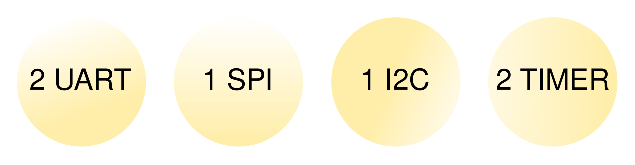
\includegraphics[width=.5\linewidth]{../figures/code/périphériques}
\end{figure}

\clearpage

\subsubsection{Timers}
Lors de cette section, 2 timers vont être configurés, ceux-ci ont des utilités différentes :

\begin{table}[h]
\begin{tabular}{lll}
	\textbf{Timer 1} & sert pour les attentes bloquantes précises. & 1 [$ms$] \\
	\textbf{Timer 2} & gère les délais entre les mesures et l'affichage des LEDs. & 10 [$ms$] \\
\end{tabular} 
\end{table} \vspace*{-5pt}

\underline{Dimensionnement timer 1}

$f_{sys} = 72\;MHz$

$f_{per} = 1\;kHz$

$presc = 8\;[-]$ \vspace*{-5pt}

\begin{equation*}
	C_{T1} = \frac{f_{sys}}{f_{per}*presc} - 1 = \frac{72*10^{6}}{1*10^{3}*8} - 1 = 8'999\; [-]
\end{equation*}


\underline{Dimensionnement timer 2}

$f_{sys} = 72\;MHz$

$f_{per} = 100\;Hz$

$presc = 16\;[-]$ \vspace*{-5pt}

\begin{equation}
	C_{T1} = \frac{f_{sys}}{f_{per}*presc} - 1 = \frac{72*10^{6}}{100*16} - 1 = 44'999\; [-]
\end{equation}

\begin{figure}[h]
	\centering
	\fbox{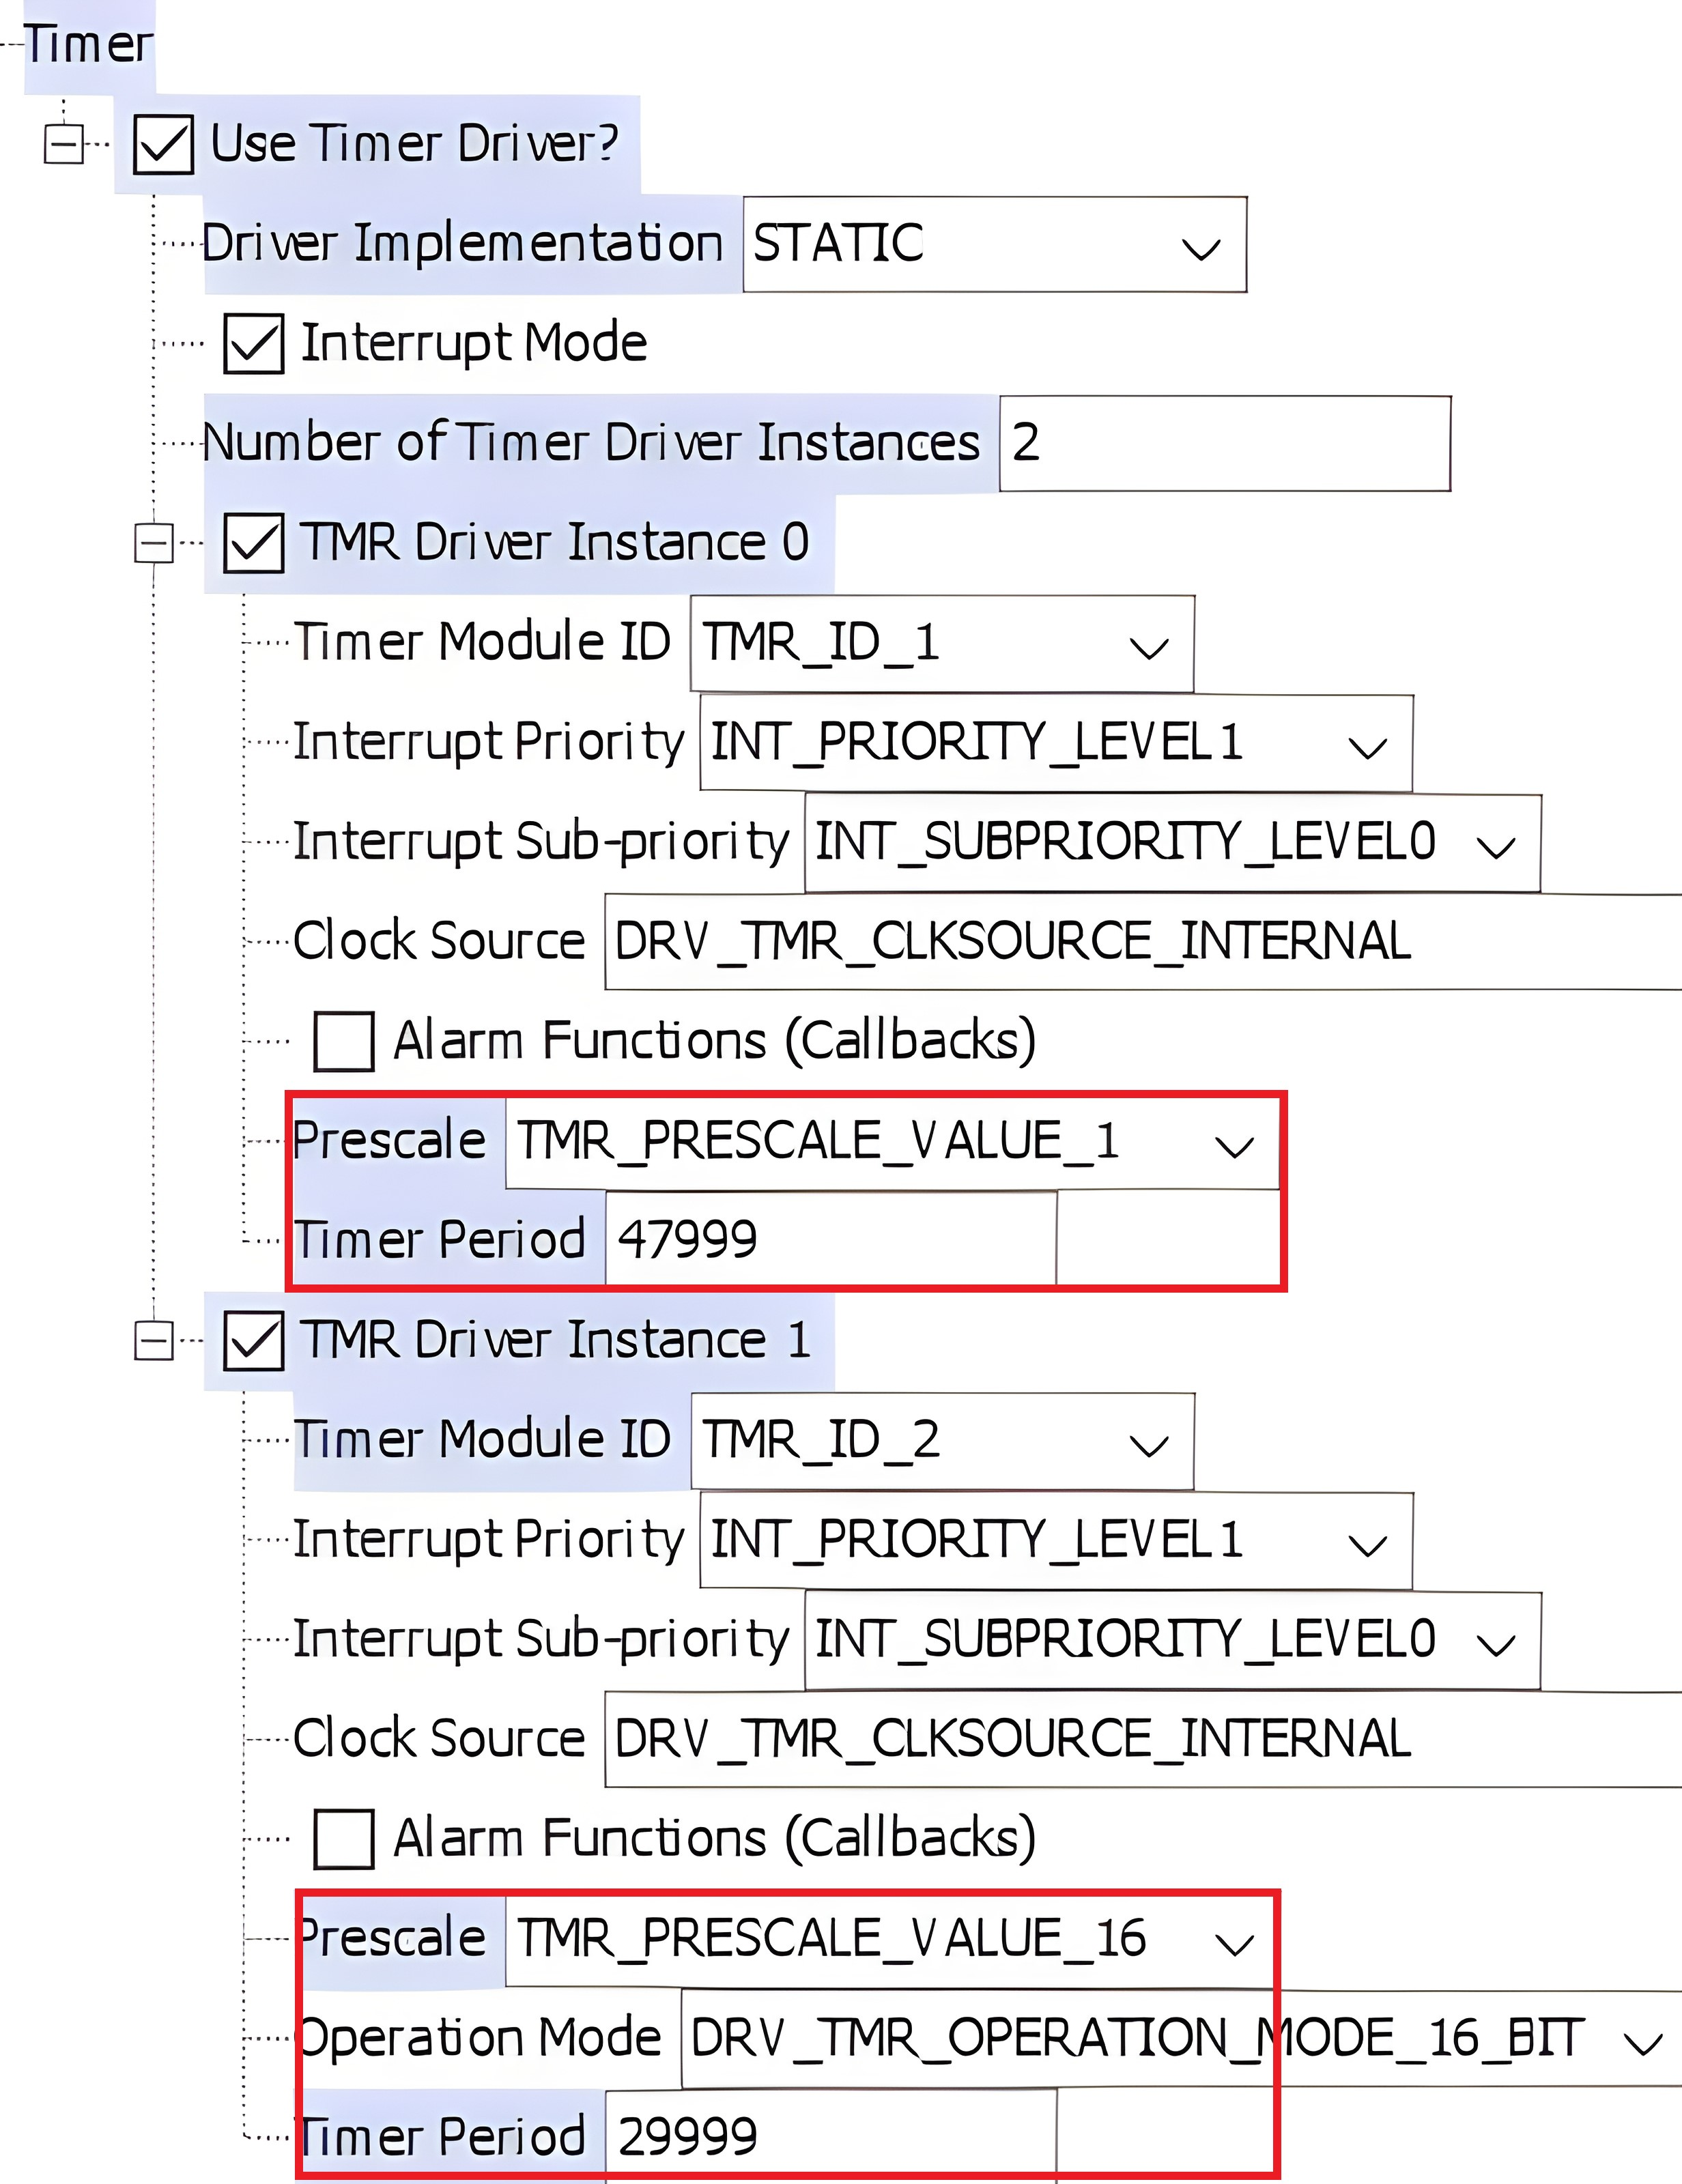
\includegraphics[width=.5\linewidth]{../figures/code/harmony/timers}}
	\caption{Configuration des timers.}
	\source{Auteur}
	\label{fig:timers}
\end{figure}

\clearpage

\begin{code}
\caption{Interruption \textbf{timer 1}, 1 [$ms$]}
\label{code:int-t1}
\begin{minted}[breaklines]{c}
void delayTimer_callback(){
	/* Increment delay timer */
	timeData.delayCnt ++;
}
\end{minted}
\end{code}

\begin{code}
\caption{Interruption \textbf{timer 2}, 10 [$ms$]}
\label{code:int-t2}
\begin{minted}[breaklines]{c}
void stateTimer_callback()
{
	/* Increment all counters */
	timeData.ledCnt ++;
	timeData.measCnt[BNO055_idx] ++;
	timeData.measCnt[GNSS_idx] ++;
	timeData.tmrTickFlag = true;
	/* When the button is pressed, the hold time is counted. */
	if(timeData.flagCntBtnPressed){
		timeData.cntBtnPressed++;
	}
	/* Do debounce on button every 10 ms */
	DoDebounce(&switchDescr, ButtonMFStateGet());
	/* Start a measure set each IMU period */        
	if ( ( timeData.measCnt[BNO055_idx] % (timeData.measPeriod[BNO055_idx]/10) ) == 0)
	timeData.measTodo[BNO055_idx] = true;
	
	/* Start a measure set each GNSS period */        
	if ( ( timeData.measCnt[GNSS_idx] % (timeData.measPeriod[GNSS_idx]/10) ) == 0)
	timeData.measTodo[GNSS_idx] = true;
	/* Manage LED if enabled */
	if((timeData.ledCnt >= LED_PERIOD) && (appData.ledState == true))
	LED_BOff();
} 
\end{minted}
\end{code}	

Dans le code \ref{code:int-t2}, nous pouvons voir le code de la routine d'interruption du timer 2. Lors de cette interruption, les différents compteurs de mesures sont incrémentés et différentes conditions vont tester si la période de mesure est atteinte. Une gestion du bouton a également lieu, notamment une mesure du temps d'appui, et une limitation des effets de rebonds mécaniques sur les signaux électriques observés par le \gls{mcu} par un échantillonnage diminué. Enfin, la LED de vie est gérée, notamment son temps allumé.

\clearpage

\subsubsection{USARTs}

Deux bus de communication UART ont dû être configurés dans le cadre de ce projet ; ceux-ci ont des utilités différentes.

\begin{center}
	\underline{Configuration des UARTs}
	\begin{table}[h]
		\centering
		\begin{tabular}{llllll}
			ID du BUS & Utilité & Baudrate & Interruption & Trame & Parité \\ 
			\hline
			UART ID1 & Réceptions commandes USB & 9600 & Priorité 1 & 8bits + 1stop & Non \\
			UART ID2 & Communication avec le \gls{gnss} & 9600 & Non & 8bits + 1stop & Non \\
		\end{tabular}
		\caption{}
		\label{tab:Usarts}
	\end{table}
\end{center}

L'USART ID1, mentionné dans le tableau \ref{tab:Usarts}, est configuré avec une interruption. Celle-ci a été mise en place afin d'implémenter un mécanisme de FIFO associé à un tampon de réception. Ceci facilite le traitement des données et évite leur perte lors de réceptions consécutives.

\subsubsection{Carte SD}
Harmony permet de configurer directement un périphérique carte-SD avec le bus SPI.
\begin{figure}[!h]
	\centering
	\begin{subfigure}[b]{0.5\textwidth}
		\centering
		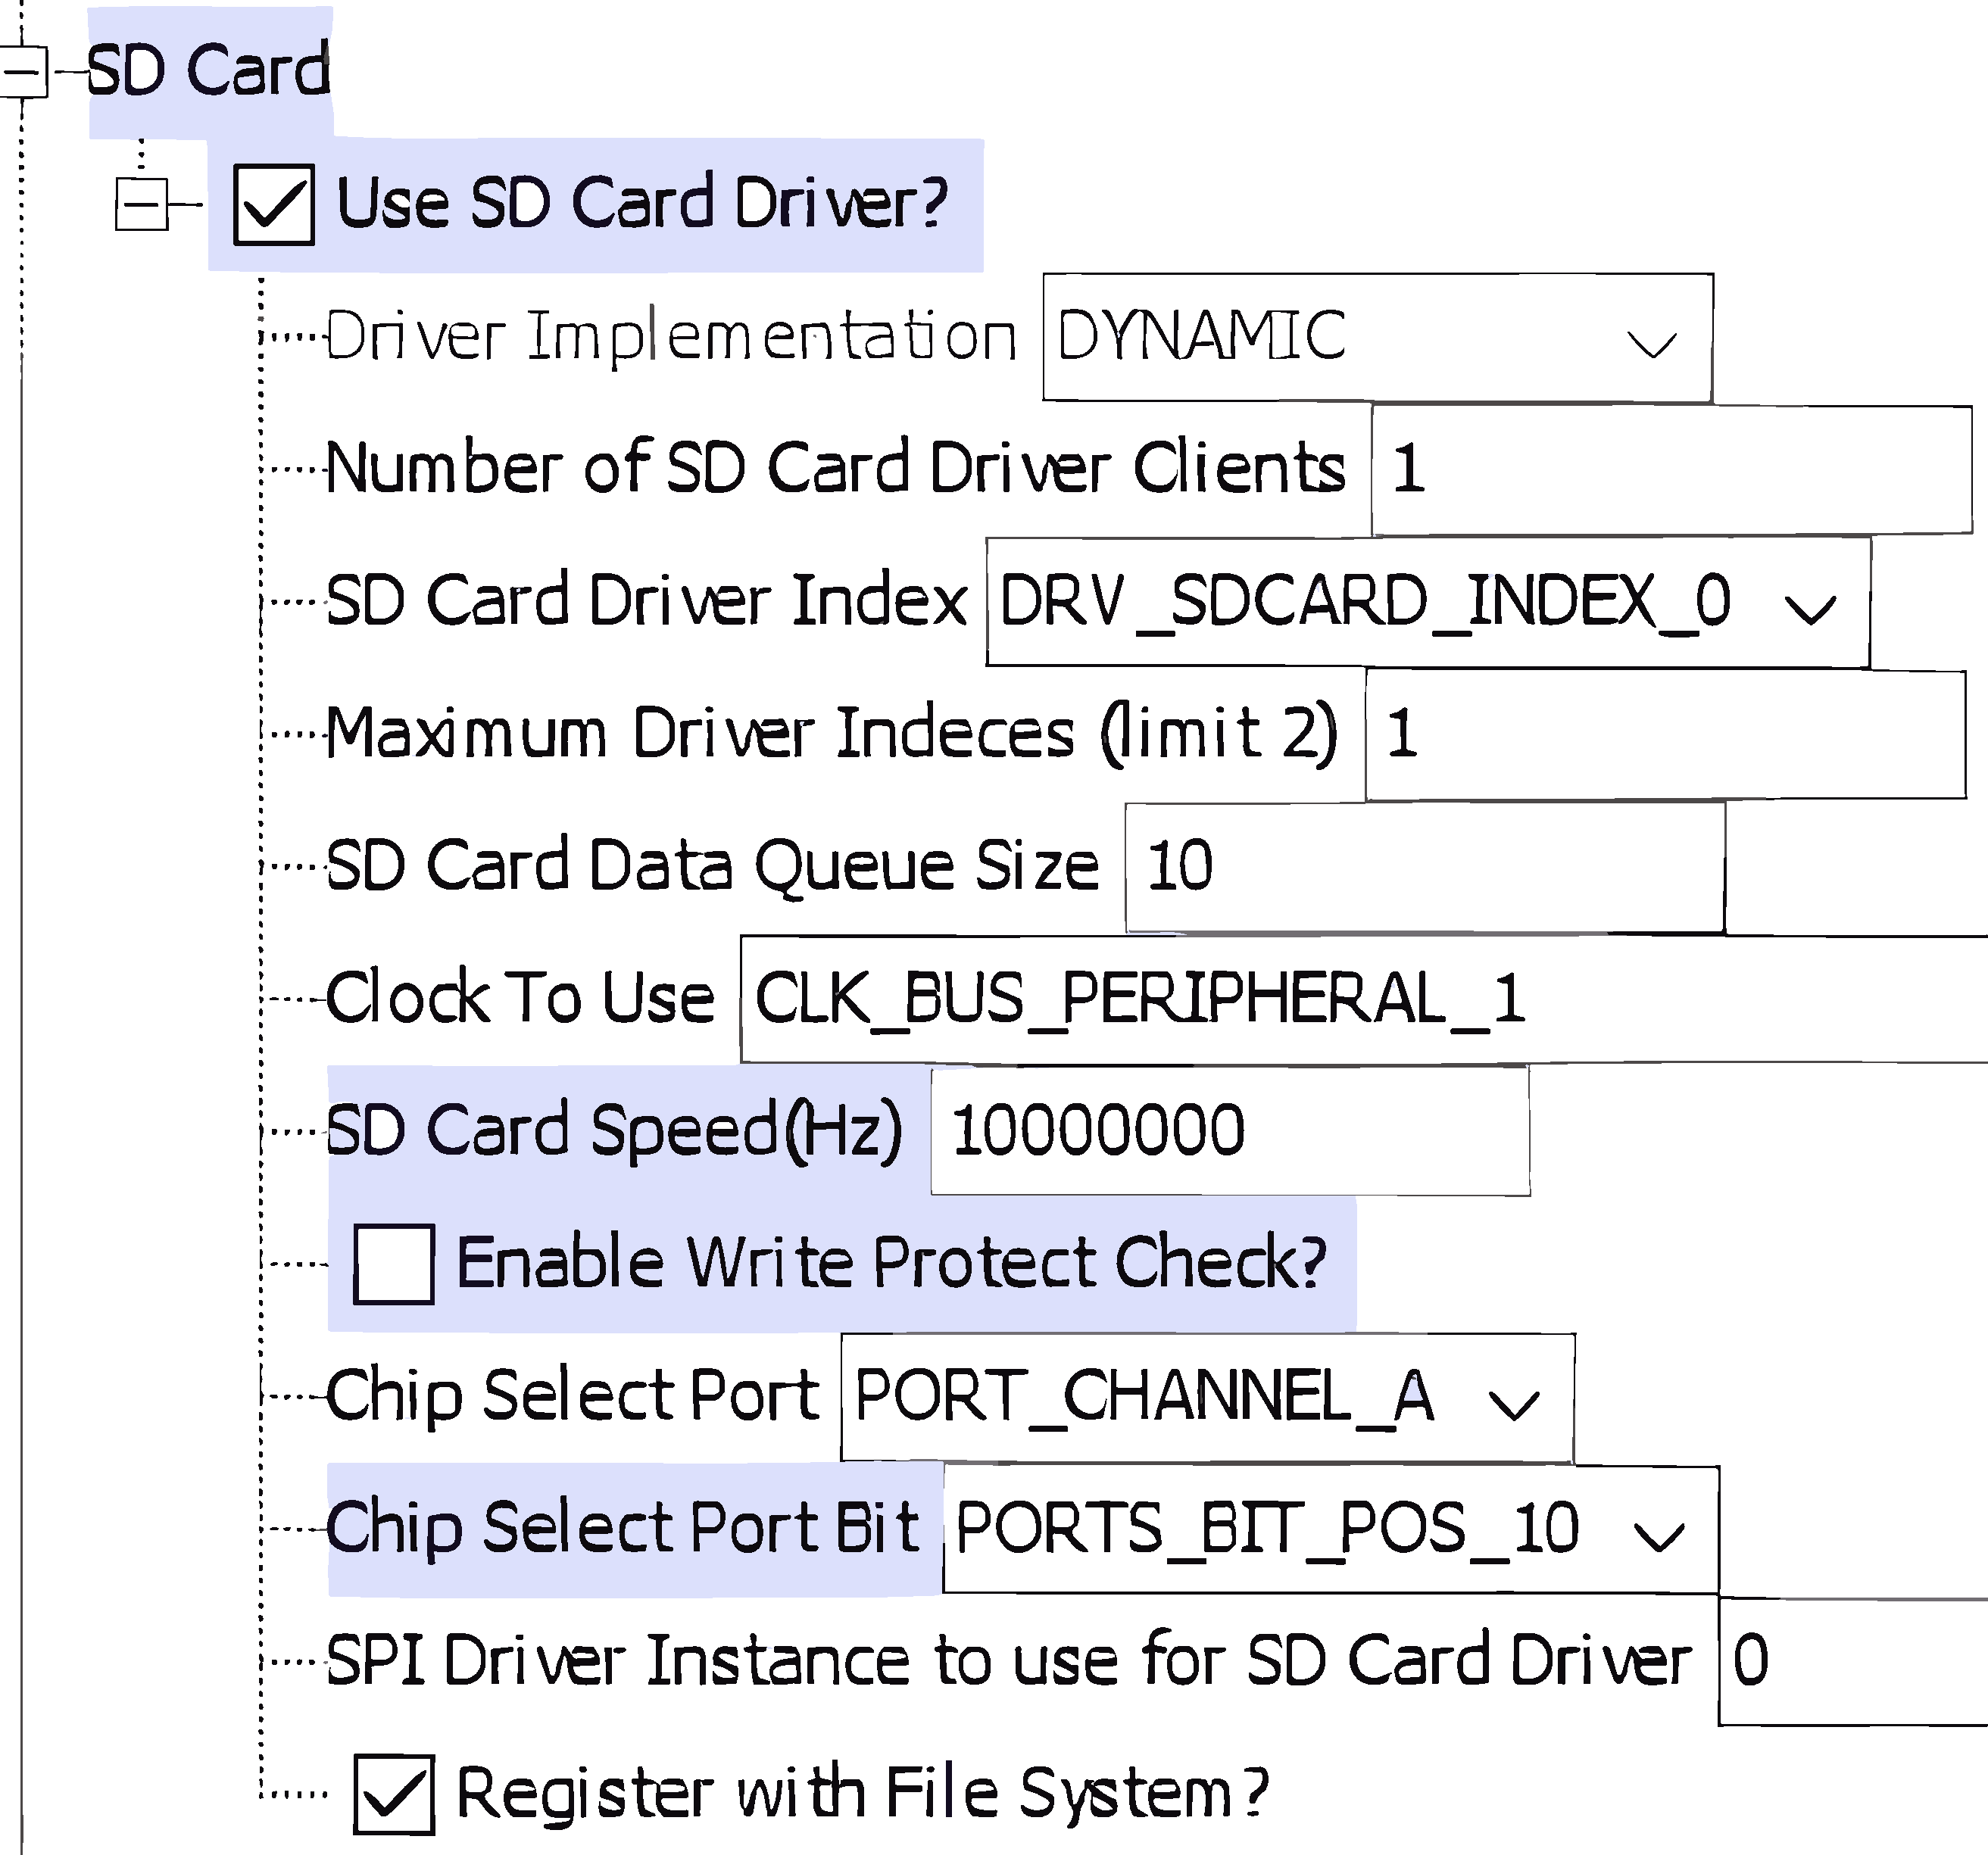
\includegraphics[width=\linewidth]{../figures/code/harmony/SD-card}
		\caption{Configuration Carte SD.}
		\label{fig:sd-card}
	\end{subfigure}
	\hfill
	\begin{subfigure}[b]{0.44\textwidth}
		\centering
		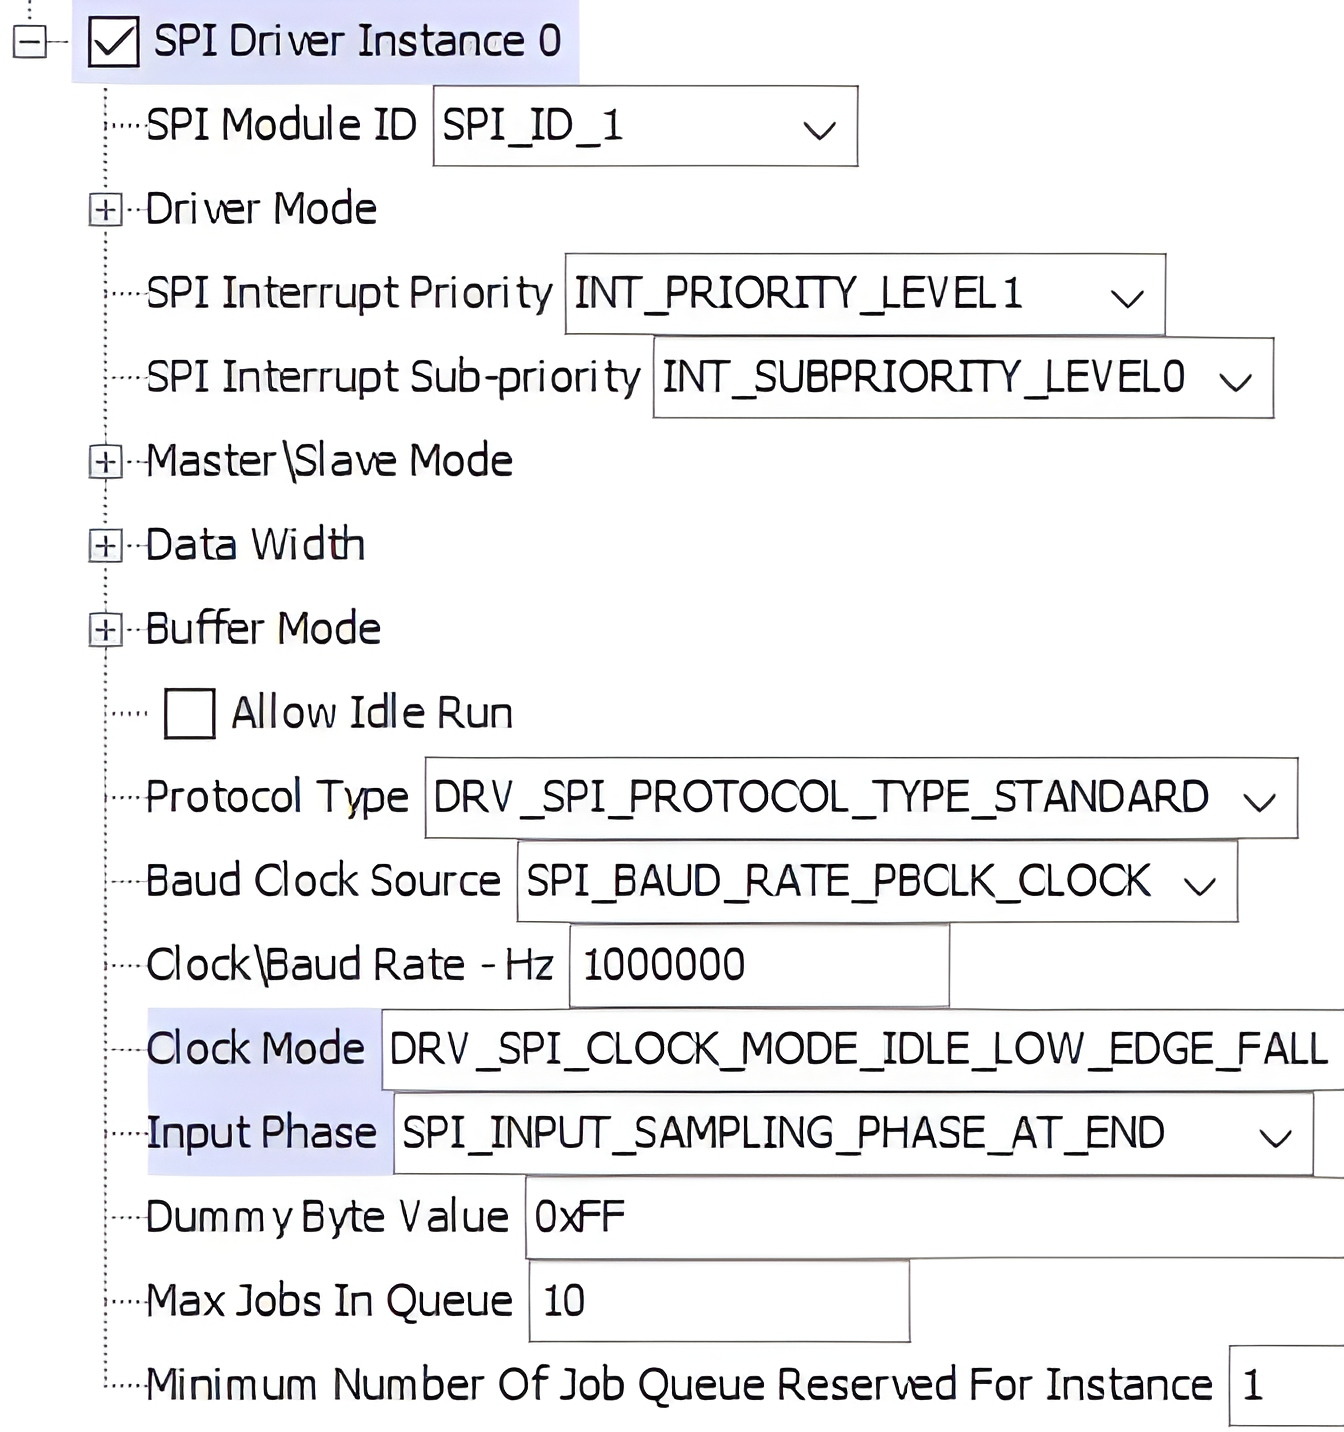
\includegraphics[width=\linewidth]{../figures/code/harmony/SD-card-spi}
		\caption{Configuration SPI.}
		\label{fig:sd-card-spi}
	\end{subfigure}
	\hfill
	\caption{Harmony, driver carte-SD.}
	\label{fig:HDriverSD}
	\source{Auteur}
\end{figure}

Sur la figure \ref{fig:sd-card}, on peut observer la configuration de la carte SD. La broche de \textit{Chip Select} est attribuée à \textbf{RA10}, qui correspond à \textbf{CS\_SD} sur le schéma présenté à la figure \ref{fig:mcu}. La connexion est établie avec une fréquence de \textbf{10MHz}.

Concernant la figure \ref{fig:sd-card-spi}, les spécificités du bus SPI y sont configurées, incluant le mode de l'horloge et la phase de l'échantillonnage. Ces configurations ont été adaptées en adéquation avec les protocoles des cartes SD\footnote{\href{https://www.renesas.com/us/en/document/apn/sd-memory-card-interface-using-spi}{SD Memory Card Interface Using SPI}.}.


\clearpage

\subsection{Application principale} 

Lors de cette section nous allons décrire le fonctionnement principale du système sous la forme d'un diagramme d'état sur la figure \ref{fig:stateapp}.

\begin{figure}[h]
	\centering
	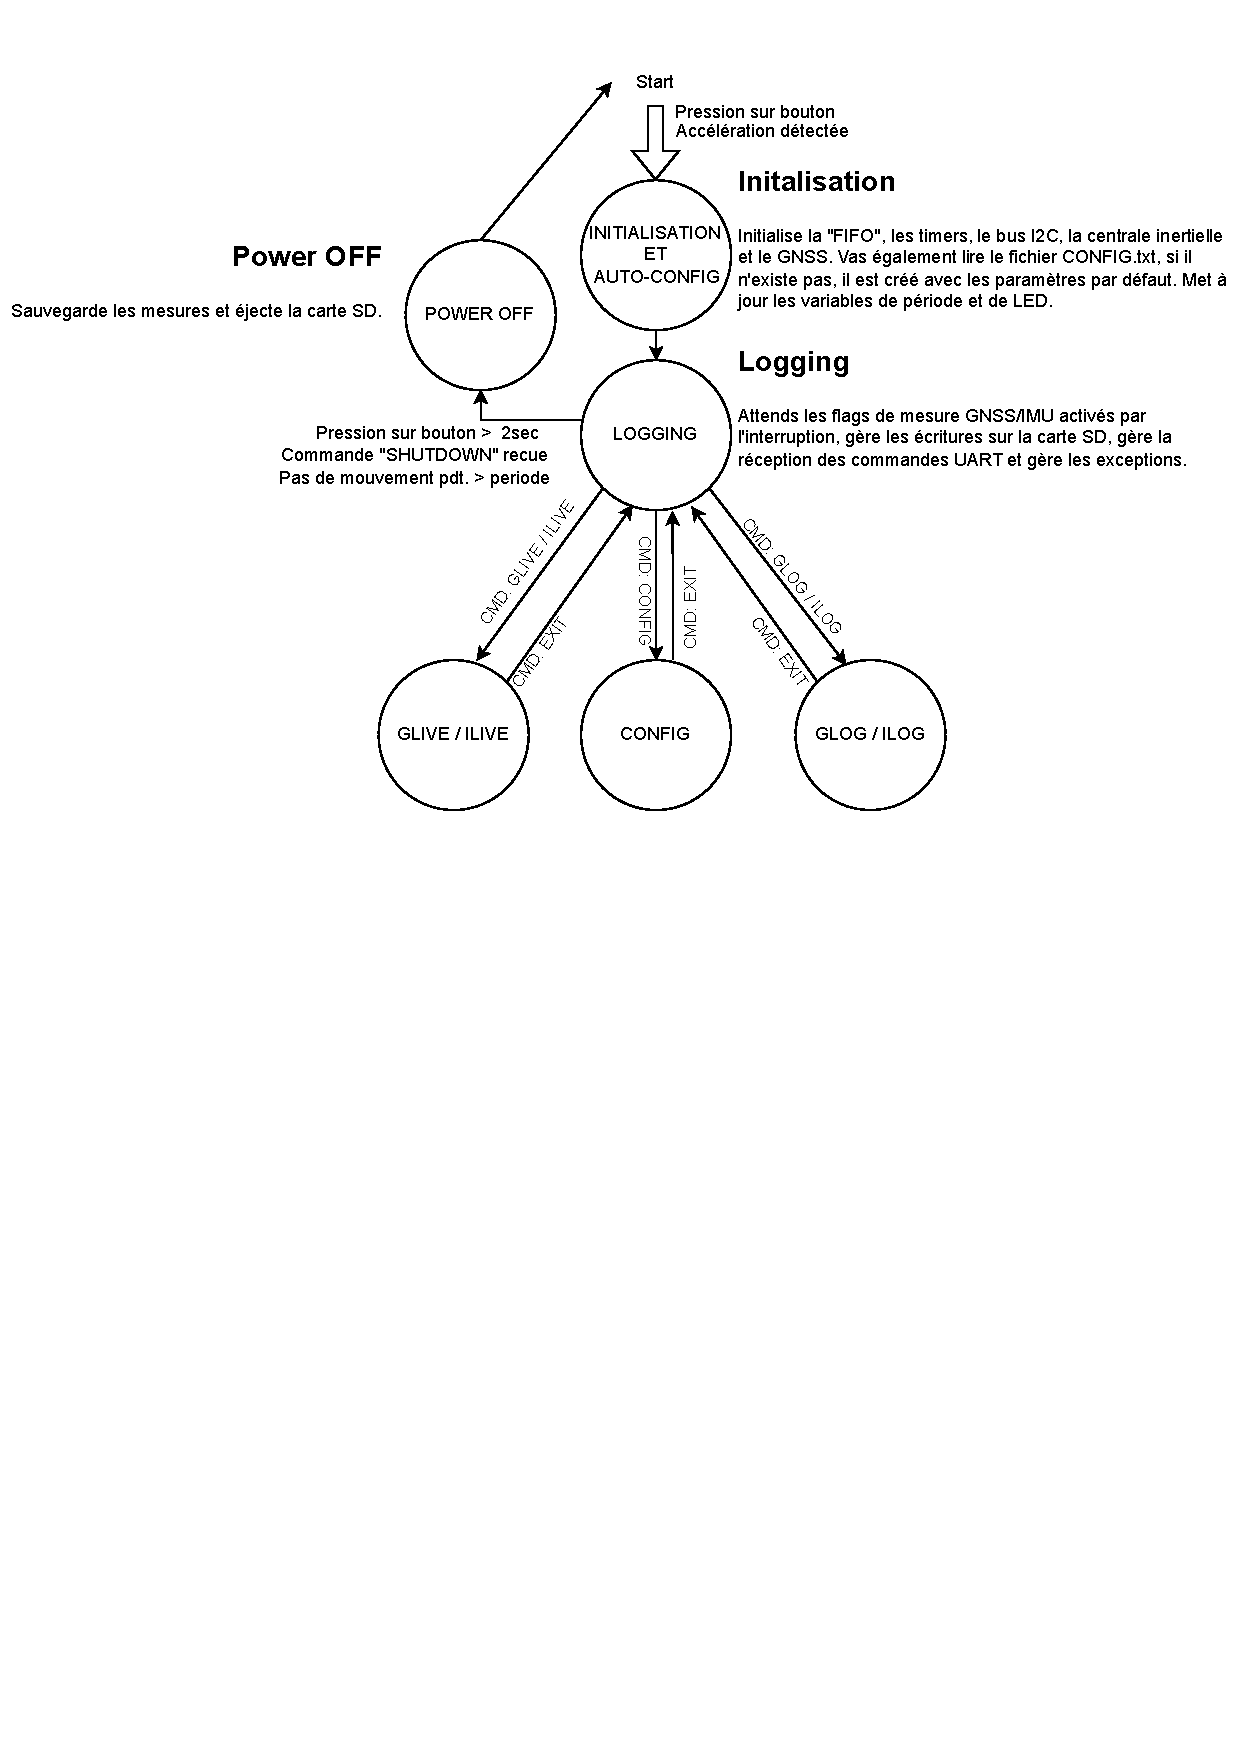
\includegraphics[width=1\linewidth]{../figures/code/diagrammes/state_app}
	\caption{Diagramme d'état principal.}
	\label{fig:stateapp}
	\source{Auteur}
\end{figure}

\subsubsection{Commandes USB-UART}
Les commandes permettent d'interagir avec le système et de manipuler les différentes données de la boîte noire.

\begin{center}
	\underline{Liste des commandes}
	\begin{table}[h]
		\centering
		\resizebox{\textwidth}{!}{
			\begin{tabular}{llll}
			GLIVE & -LVG & : & Permet d'afficher les données du \gls{gnss} en live sur le terminal sans les enregistrer. \\
			ILIVE & -LVI & : & Lance l'envoi des données live de l'\gls{imu} sans les enregistrer. \\
			GLOG & -GL & : & Envoie les données de localisation de la carte-SD au terminal. \\
			ILOG & -IL & : & Envoie les données inertielle de la carte-SD au terminal.\\
			GCLR & -GC & : & Supprime les logs du \gls{gnss}.\\
			ICLR & -IC & : & Supprime les logs de l'\gls{imu}.\\
			EXIT & X & : & Quitte le mode en cours.\\
			SHUTDOWN & -OFF & : & Sauvegarde et éteint le système. \\
			CONFIG & -CFG & : & Démarre le mode de configuration du système. \\
			\faChevronRight & INTG:XXXX & : & Dans mode config. permet de régler la période de mesure du \gls{gnss}.\\
			\faChevronRight & INTI:XXXX & : & Dans mode config. permet de régler la période de mesure de l'\gls{imu}. \\
			\faChevronRight & LEDV:X & : & Dans mode config. permet d'activer ou non la LED de vie. \\
			\faChevronRight & TOFF:XX & : & Dans mode config. permet de fixer le temps d'inactivité (éteint le système).
		\end{tabular}
		}
		\caption{Commandes disponibles}
		\label{tab:cmdDisp}
	\end{table}
\end{center}

Les commande de la table \ref{tab:cmdDisp} peuvent également être envoyés en caractères minuscules.

\clearpage

Sur la figure \ref{fig:sequence-app}, la séquence de la boucle principale de l'application est représentée. Celle-ci interagit avec les différents périphériques en utilisant diverses bibliothèques C.

\begin{figure}[!h]
	\centering
\	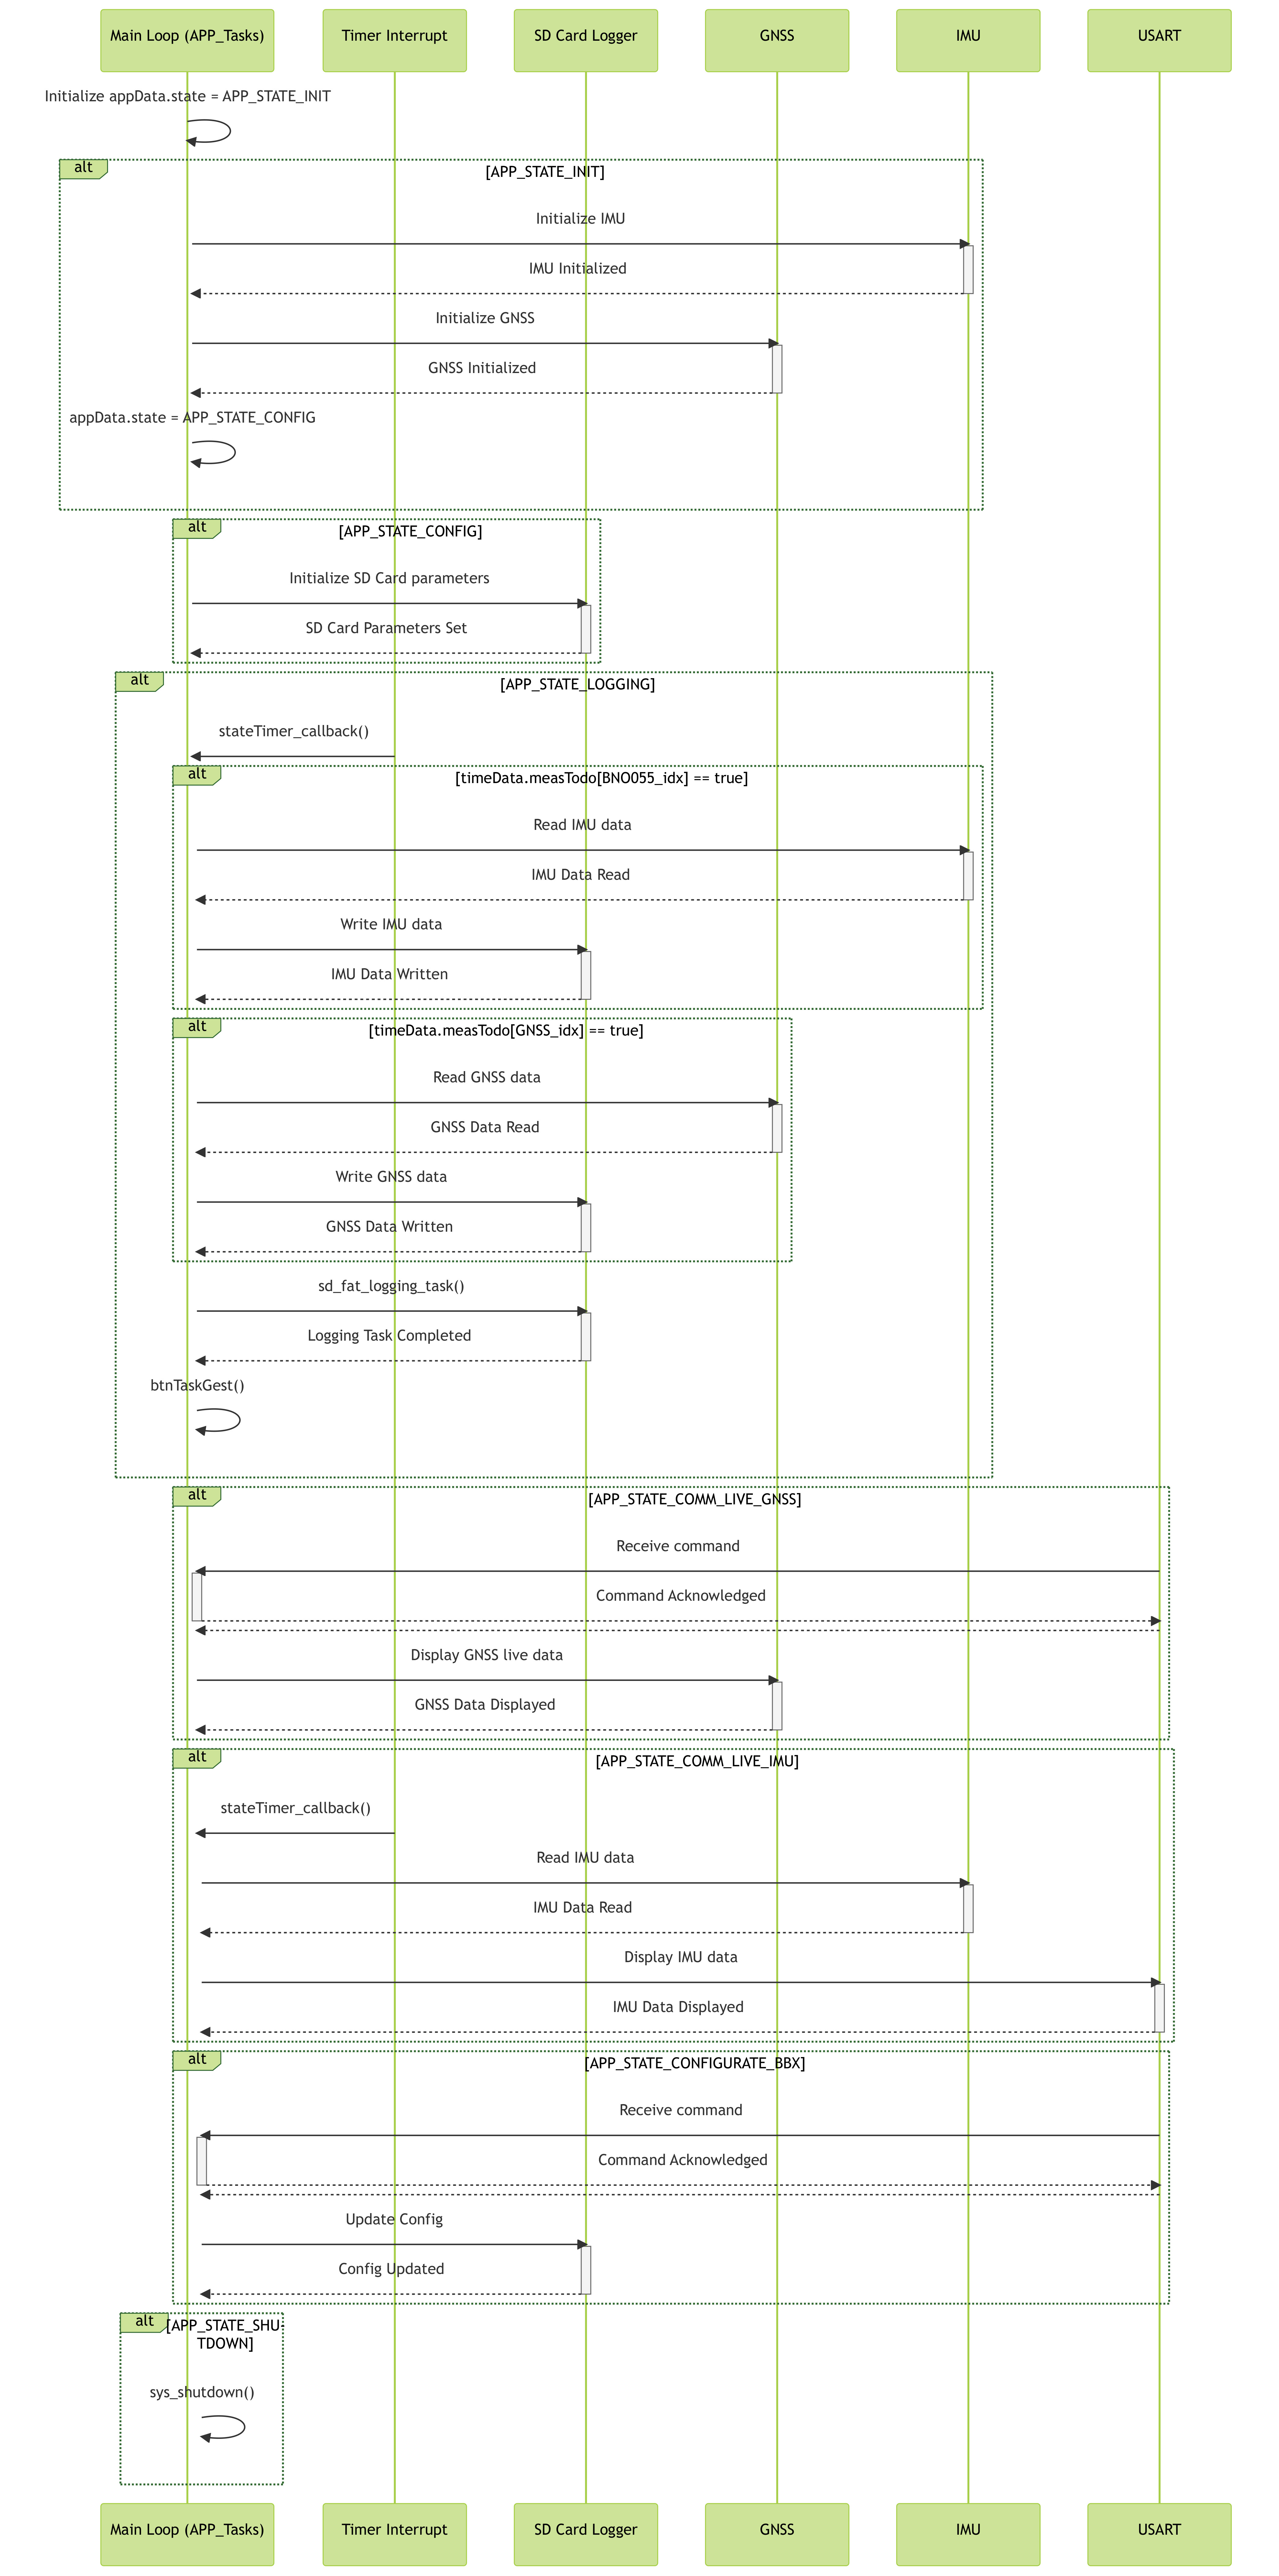
\includegraphics[width=.96\linewidth]{../figures/code/diagrammes/sequence-app}
	\caption{Diagramme de séquence principal.}
	\label{fig:sequence-app}
	\source{Auteur}
\end{figure}

\clearpage
\subsubsection{État de logging du système}
L'état de logging est représenté par un flowchart sur la figure \ref{fig:pdfresizer}.

\begin{figure}[!h]
	\centering
	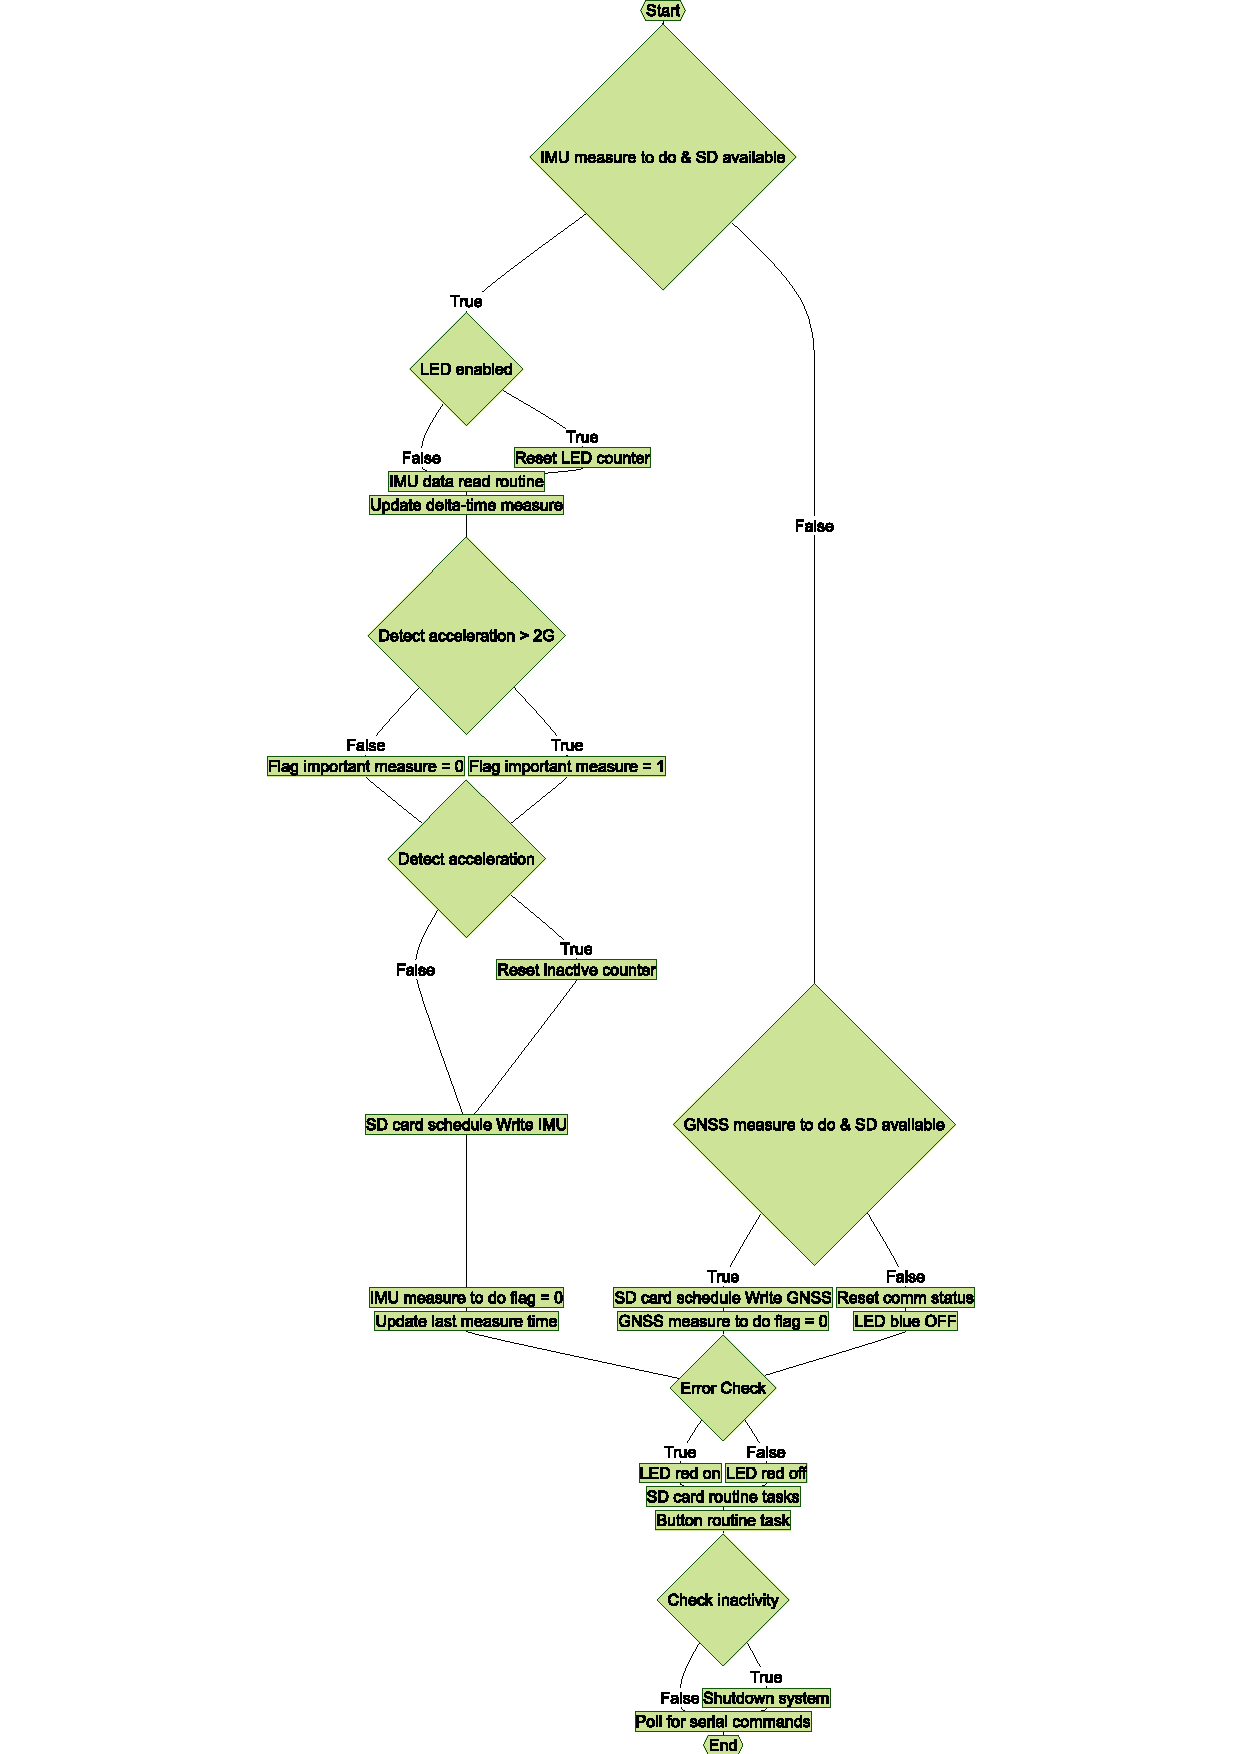
\includegraphics[width=.95\textwidth]{../figures/code/diagrammes/logging-flowchart}
	\caption{Flowchart de l'état de logging.}
	\label{fig:pdfresizer}
	\source{Auteur}
\end{figure}

\clearpage

\subsection{Carte SD}
Le code de gestion de fichier de la carte SD est divisé en deux machines d'états. La première est dédiée à l'initialisation, à la lecture et à la modification du fichier de configuration. La seconde s'occupe du logging et de l'enregistrement des mesures dans des fichiers distincts. Ces machines d'états sont non-bloquantes et doivent être appelées périodiquement pour permettre une routine de gestion de la carte SD.

\subsubsection{Carte SD : initialisation et configuration}

La machine d'état initiale est appelée lorsqu'elle se trouve dans l'état \textbf{APP\_STATE\_CONFIG}, comme illustré sur la figure \ref{fig:sequence-app}. Elle continuera d'être appelée jusqu'à ce qu'elle atteigne l'état \textbf{\textit{IDLE}}. Notons également que cette machine d'état est sollicitée en mode configuration (\textbf{\textit{init = false}}) durant l'état \textbf{APP\_STATE\_CONFIGURATE\_BBX}, visible sur la même figure \ref{fig:sequence-app}. Ce processus est représenté sous forme de diagramme d'état à la figure \ref{fig:sd-card-init}



\begin{figure}[h]
	\centering
	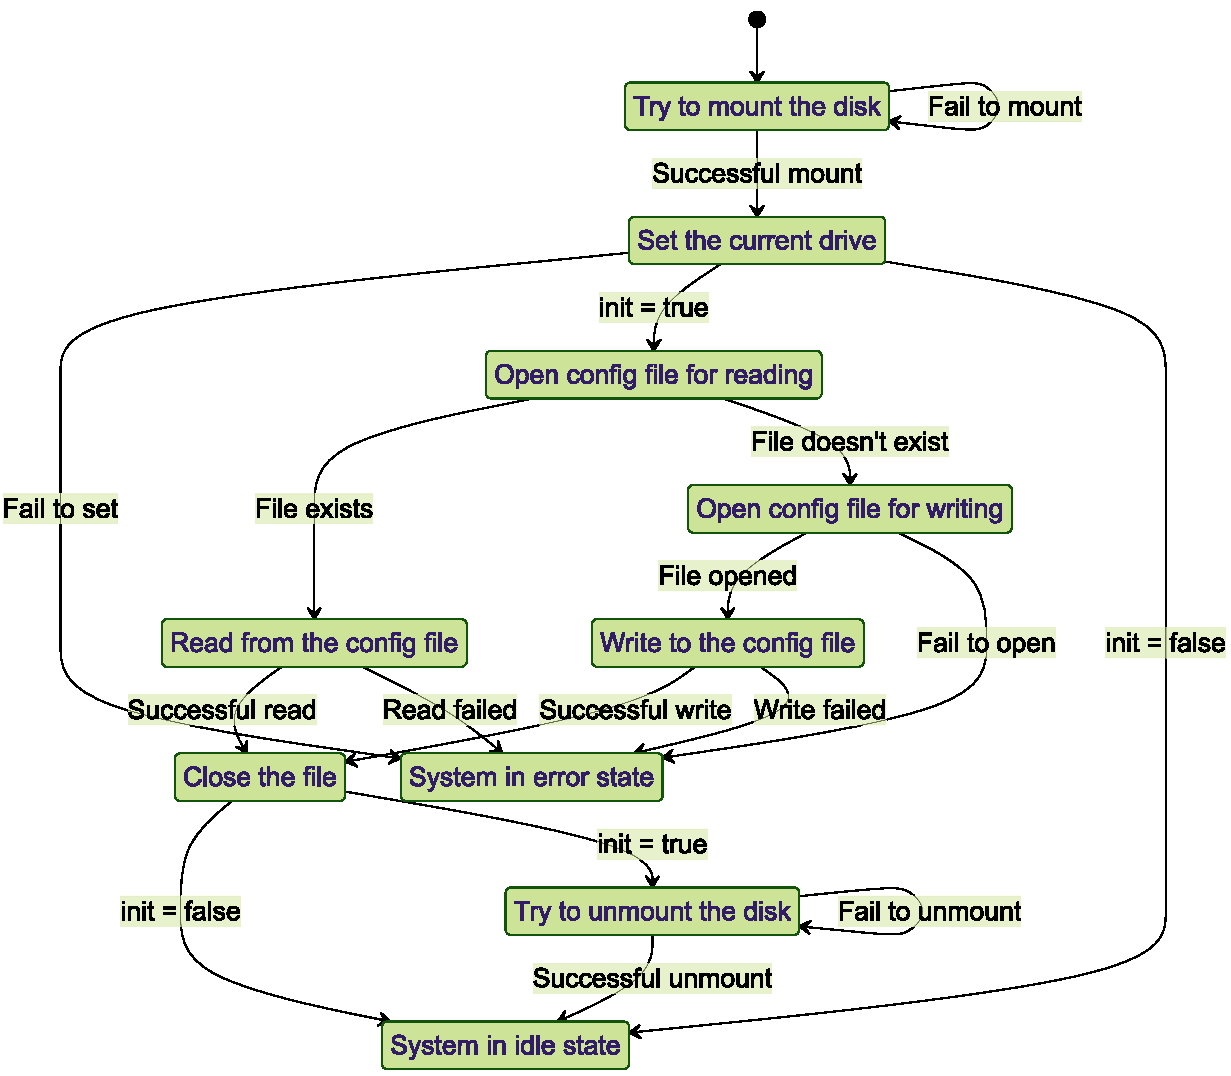
\includegraphics[width=1\linewidth]{../figures/code/diagrammes/sd-card-Init}
	\caption{Application carte SD initialisation/config.}
	\label{fig:sd-card-init}
	\source{Auteur}
\end{figure}

\clearpage

\subsubsection{Carte SD : écriture des données}
Cette machine d'état est systématiquement appelée lorsque le système se trouve dans l'état \textbf{APP\_STATE\_LOGGING}, comme illustré sur la figure \ref{fig:sequence-app}. Ceci est réalisé via la fonction \verb*|sd_fat_logging_task()|. Pour programmer des écritures et interagir avec cette machine d'état, deux fonctions d'interface sont utilisées : \verb*|sd_IMU_scheduleWrite()| qui permet de planifier l'écriture de données de l'\gls{imu}, et \verb*|sd_GNSS_scheduleWrite()| pour l'écriture des données du \gls{gnss}.

\begin{figure}[h]
	\centering
	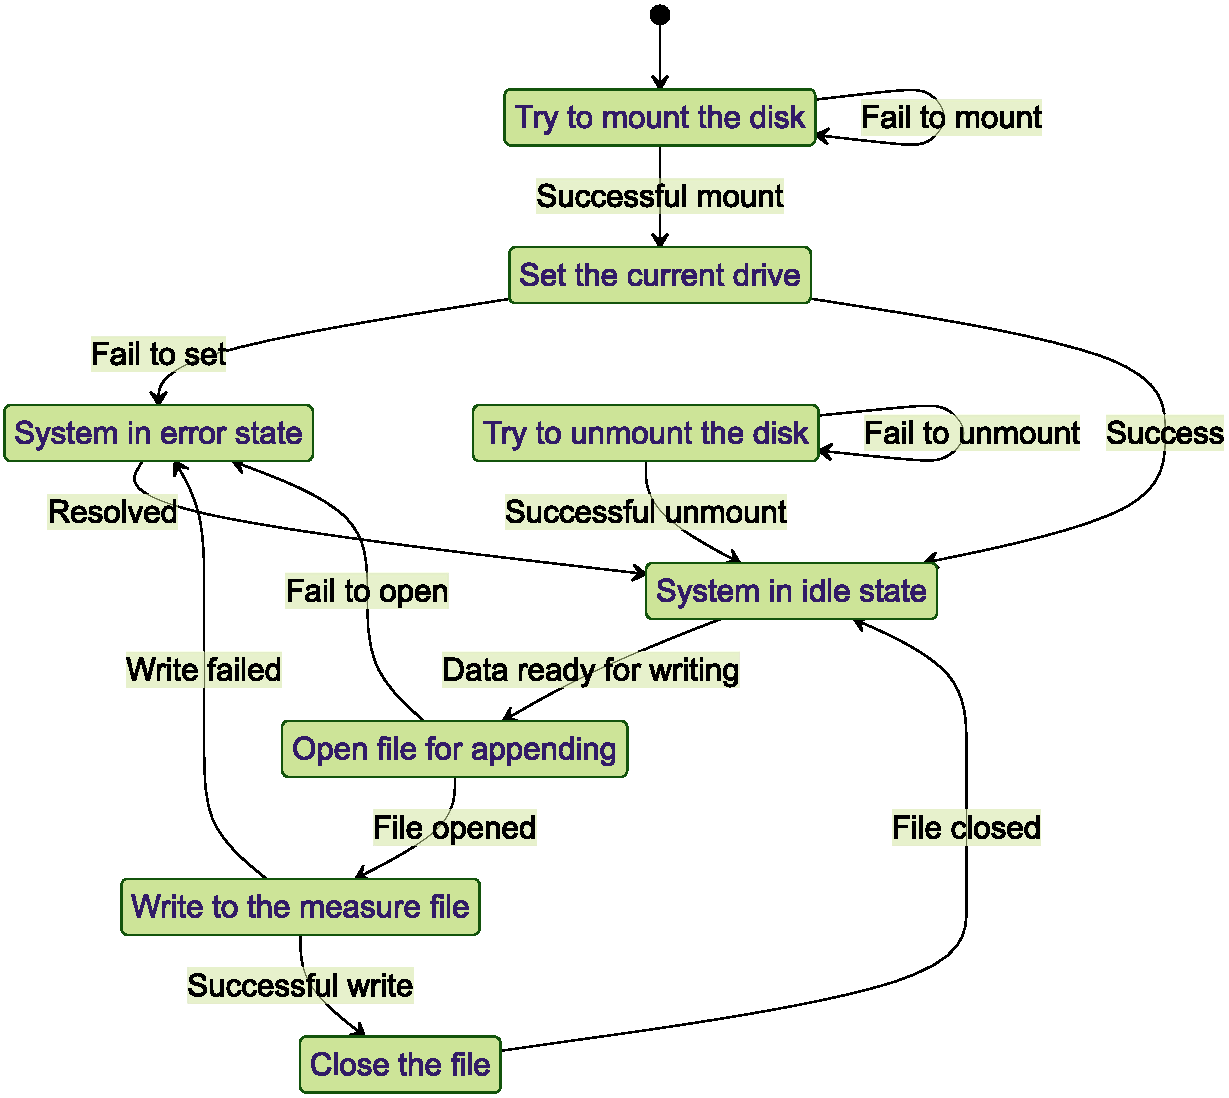
\includegraphics[width=.85\linewidth]{../figures/code/diagrammes/sd-card-logging}
	\caption{Machine d'état logging.}
	\label{fig:sd-card-logging}
	\source{Auteur}
\end{figure}

\begin{figure}[h]
	\centering
	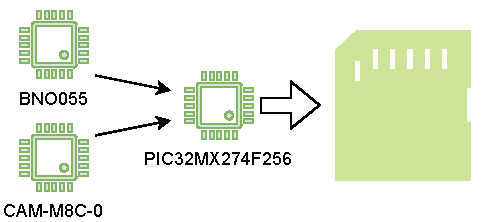
\includegraphics[width=0.46\linewidth]{../figures/code/Illustration-SD-per}
	\caption{Illustration des interactions.}
	\label{fig:illustration-sd-per}
	\source{Auteur}
\end{figure}

\clearpage

\subsection{Centrale inertielle}
Lors de cette section, nous allons décrire les différents aspects de la mise en place de la centrale inertielle \fbox{\href{https://www.bosch-sensortec.com/products/smart-sensors/bno055/}{BNO055}}.

\paragraph*{Interfaçage de l'\gls{imu}}
Bosch propose une librairie\footnote{\href{https://github.com/BoschSensortec/BNO055_driver}{https://github.com/BoschSensortec/BNO055\_driver}} d'APIs pour communiquer avec la centrale inertielle. Cette librairie est accompagnée d'un fichier \textit{support} qui sert à lier les fonctions de protocoles aux fonctions bas niveau du bus de communication I2C.


\subsubsection{Initialisation}

\begin{center}
	\underline{Procédure d'initialisation}
	\begin{table}[h]
		\centering
		\begin{tabular}{ll}
			$\star$ \oldstylenums{1} & Réinitialisation hardware par la pin RESET pendant 100ms. \\
			$\star$ \oldstylenums{2} & Désactivation de l'interruption\footnotemark de l'\gls{imu}. \\
			$\star$ \oldstylenums{3} & Attribution des fonctions bas niveau dans les pointeurs de la librairie. \\
			$\star$ \oldstylenums{4} & Obtention des informations du BNO055 (IDs, Version...). \\
			$\star$ \oldstylenums{5} & Attribution du mode d'alimentation "Normal". \\
			$\star$ \oldstylenums{6} & Choix du mode d'opération "AMG" (pour lecture simple Accel. magnitude et gyro.). \\
			$\star$ \oldstylenums{7} & Lecture initiale à vide, d'initialisation (Accel. magnitude gyroscope.). \\
			$\star$ \oldstylenums{6} & Choix du mode d'opération "NDOF" (pour lecture des données de fusions complexes.). \\
			$\star$ \oldstylenums{7} & Lecture initiale à vide, d'initialisation (Euler, Quaternion, gravité et accel. linéaire). \\
			$\star$ \oldstylenums{8} & Programmation de l'interruption du BNO055 pour la détection d'une certaine accélération.
		\end{tabular}
	\end{table}
\end{center}
\footnotetext{Reset toutes les sources d'interruptions de l'\gls{imu} dans le registre 0x3F bit 6. }
\vspace*{-15mm}

\subsubsection{Lecture des données}

La phase cruciale concernait l'initialisation du BNO055. La lecture des diverses valeurs est assurée par une fonction spécifiquement créée, nommée \verb*|bno055_read_routine()|. Cette fonction récupère les données suivantes : Quaternion WXYZ, magnitude XYZ, gyroscope XYZ, angles d'Euler HPR, accélération linéaire XYZ, et gravité XYZ. Ces données son stockées dans une structure locale au fichier \textit{app.c} et possède la structure suivante :

\begin{minted}{c}
typedef struct {
	s32 comres;
	bool flagMeasReady;
	uint8_t flagImportantMeas;
	struct bno055_gravity_double_t gravity;
	struct bno055_linear_accel_double_t linear_accel;
	struct bno055_euler_double_t euler;
	struct bno055_gyro_double_t gyro;
	struct bno055_mag_double_t mag;
	struct bno055_quaternion_t quaternion;
	unsigned long time;
	unsigned long l_time;
	uint16_t d_time;
}s_bno055_data;
\end{minted}

\subsubsection{Système de détection de mouvements}

La centrale inertielle \textit{BNO055} permet de configurer une interruption pour un certain événement et une certaine durée. Dans cette section, nous décrirons la configuration de cette interruption pour l'enclenchement du système ainsi que la possibilité d'activer/désactiver cette option.

\begin{code}
\caption{Configuration de l'interruption}
\label{code:configInt}
\begin{minted}[breaklines]{c}
/* BNO055 motion interrupt mode */
1) bno055_set_accel_any_motion_no_motion_axis_enable (BNO055_ACCEL_ANY_MOTION_NO_MOTION_X_AXIS, 1);
2) bno055_set_accel_any_motion_no_motion_axis_enable (BNO055_ACCEL_ANY_MOTION_NO_MOTION_Y_AXIS, 1);
3) bno055_set_accel_any_motion_no_motion_axis_enable (BNO055_ACCEL_ANY_MOTION_NO_MOTION_Z_AXIS, 1);

4) bno055_set_accel_any_motion_thres(10);
5) bno055_set_accel_any_motion_durn(20);
6) bno055_set_intr_accel_any_motion(1);
7) bno055_set_intr_mask_accel_any_motion(1);	
\end{minted}
\end{code}

Les valeurs de configuration peuvent êtres définies en tant que constantes pour êtres plus facilement configurable lors de mise-à-jour firmware.

\begin{center}
	\underline{Description des lignes du code \ref{code:configInt}}
	\begin{table}[h]
		\centering
		\begin{tabular}{ll}
			$\star$ \oldstylenums{1} & Activation de l'axe X pour le mode \textit{anymotion}. \\
			$\star$ \oldstylenums{2} & Activation de l'axe Y pour le mode \textit{anymotion}. \\
			$\star$ \oldstylenums{3} & Activation de l'axe Z pour le mode \textit{anymotion}. \\
			$\star$ \oldstylenums{4} & Attribution de la valeur de déclenchement à $78.3 m\textbf{g} = 0.768 m/s^2$. \\
			$\star$ \oldstylenums{5} & Configuration de la durée à $20ms$. \\
			$\star$ \oldstylenums{6} & Active l'interruption, accélération. \\
			$\star$ \oldstylenums{7} & Masque l'interruption. \\
		\end{tabular}
	\end{table}
\end{center} \vspace*{-10mm}

\paragraph{Gestion de l'interruption} L'interruption est réinitialisée au démarrage du système ainsi que lors de sa mise en veille.
\vspace*{-4mm}
\paragraph{Mode low power} lorsque le système se met en veille, la BNO055 est configurée pour fonctionner uniquement avec son accéléromètre et son mode de puissance passe en \textit{low power}.

\begin{code}
\caption{Configuration de l'interruption}
\label{code:lowPowerBNO}
\begin{minted}[breaklines]{c}
/* Set acceleration only operation, power saving */
bno055_set_operation_mode(BNO055_OPERATION_MODE_ACCONLY);
/* set the power mode to LOW POWER */
bno055_set_power_mode(BNO055_POWER_MODE_LOWPOWER);
/* Reset interrupt pin */
bno055_set_intr_rst(1);	
\end{minted}
\end{code}

\clearpage

\paragraph{Configuration enclenchement automatique}

Le système propose deux modes d'opération : le premier permet un enclenchement automatique lors de la détection d'un mouvement, tandis que le second active le système suite à une impulsion sur le bouton. Il est à noter que pour activer le mode automatique, une première impulsion sur le bouton est nécessaire et le système doit avoir transité au moins une fois par l'état "shutdown" du code. Dans les deux modes, le système peut entrer en veille si aucun mouvement n'est détecté sur une durée configurée.

Lorsque le système est en mode d'enclenchement automatique, le circuit reste partiellement actif, ce qui engendre une consommation d'énergie détaillée ultérieurement dans la section "Validation du design". Même si la batterie est en mesure de supporter cette consommation, il reste possible de désactiver ce mode pour activer le système uniquement par le biais du bouton.

\paragraph*{Configuration} La centrale inertielle peut être alimentée soit de manière indépendante, soit avec le reste du système, influençant ainsi les modes décrits précédemment. Pour configurer ces modes, deux options sont disponibles : \vspace*{+2mm}


\begin{tabular}{lll}
	\textbf{W6} connecté & \gls{imu} alimentation autonome. & Mode accélération auto-enclenchement. \\
	\textbf{W7} connecté & Alimentation dépendant du système. & Mode enclenchement bouton uniquement. \\
	\textbf{W6} \& \textbf{W7} & \color{red}{Connexion à éviter !} & \\
\end{tabular}

\begin{figure}[h]
	\centering
	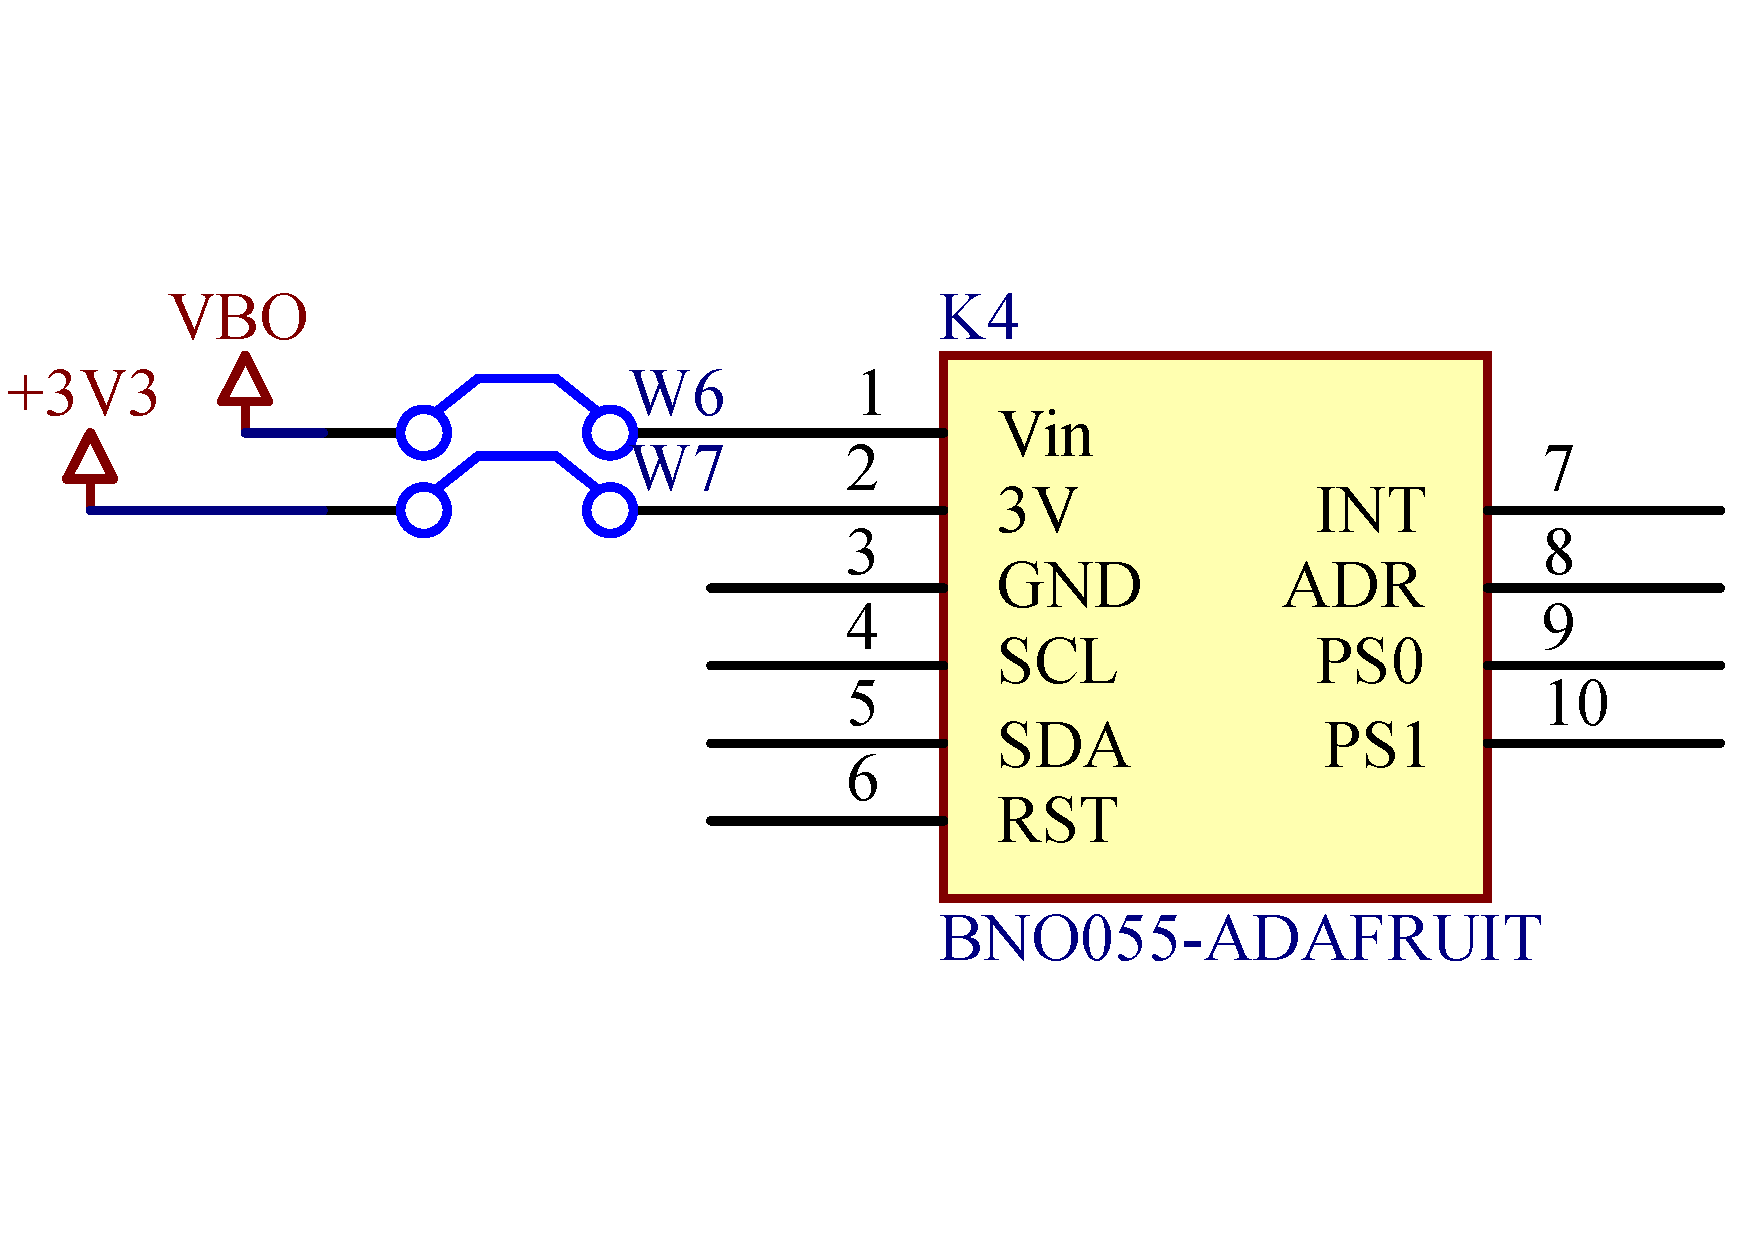
\includegraphics[width=0.7\linewidth]{../figures/code/jumper-config-mode-IMU}
	\caption{Connexions des jumber du BNO055.}
	\label{fig:jumper-config-mode-imu}
\end{figure}

\begin{figure}[h]
	\centering
	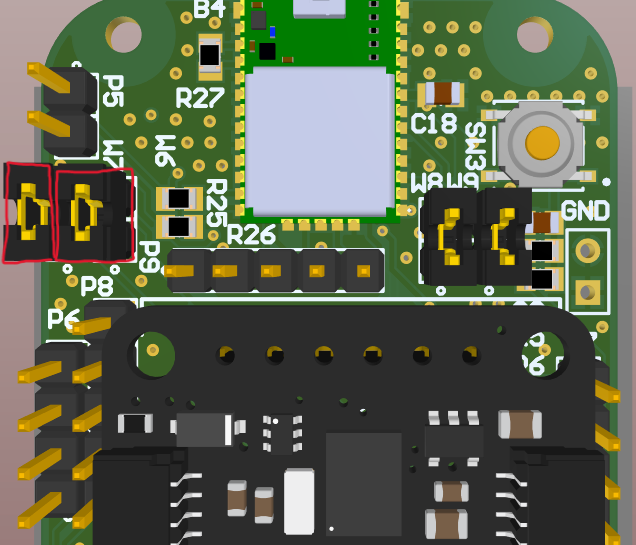
\includegraphics[width=0.5\linewidth]{../figures/code/config-mode-IMU}
	\caption{Emplacement des jumpers sur le \gls{pcb}.}
	\label{fig:config-mode-imu}
\end{figure}

Sur la figure \ref{fig:config-mode-imu}, les jumpers sont entourés en \textbf{rouge}. Le jumper \textbf{W6} se situe à droite tandis que \textbf{W7} se situe à gauche.

\clearpage	

\subsection{Format des données}

Lors de cette section, sera décrite les formats des données

\subsection{Hiérarchie des fichiers du système}






% ---------- MESURE PREUVE DE CONCEPT --------------------------- 
\clearpage

\section{Validation du design} \label{sec:Validation-design}
Dans cette section, nous décrirons la procédure de vérification des caractéristiques du projet ainsi que sa validation.

\subsection{Liste de matériel} \label{ssec:Liste-materiel}
\begin{itemize}
	\item \textbf{P1} : Oscilloscope Tektronix RTB2004 ES.SLO2.05.01.11
	\item \textbf{P2} : Multimètre GwInstek GDM-396 ES.SLO2.00.00.94
	\item Carte Mini-Boite-Noire 1924B
\end{itemize}

\subsection{Consommations}
Dans cette section, nous mesurerons les différentes consommations du système. Cette étape est importante pour caractériser le système et déterminer son autonomie.

\subsubsection{Méthode de mesure}
L'objectif est de basculer entre les différents modes (veille, logging...) de la carte et d'en mesurer la consommation. À cet effet, un ampèremètre a été placé en série avec la batterie, comme illustré à la figure \ref{fig:schema-courant}.

\subsubsection{Schéma de mesure}

\begin{figure}[h]
	\centering
	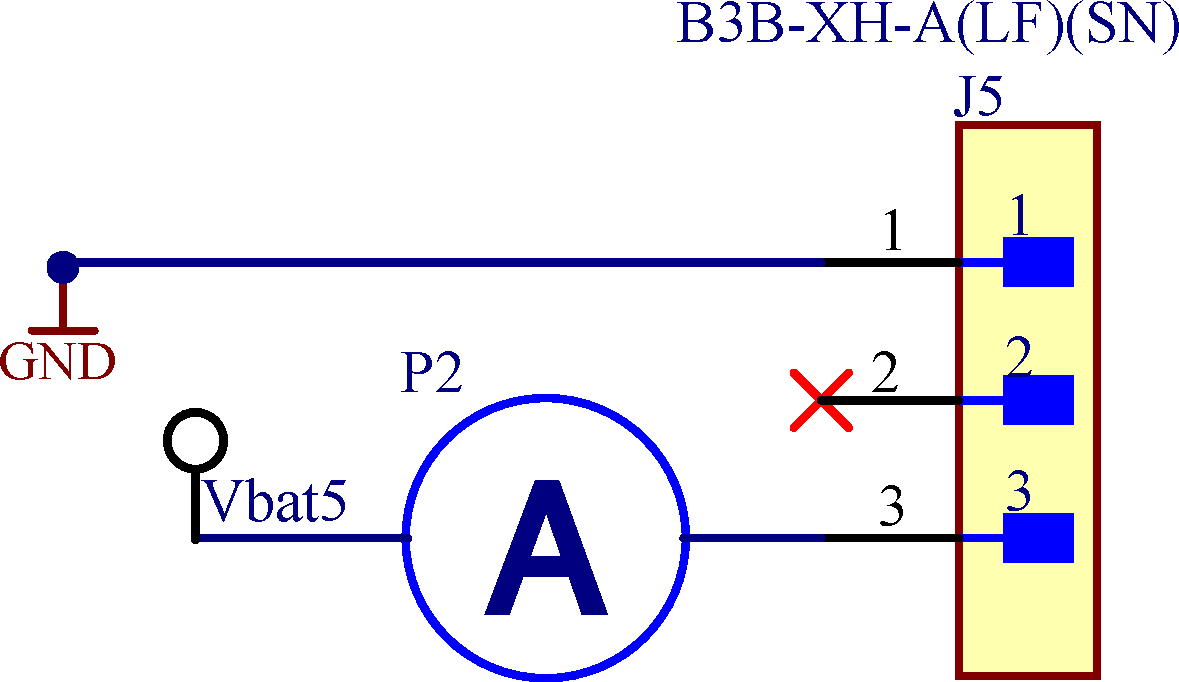
\includegraphics[width=.32\linewidth]{../figures/mesures/schema-courant}
	\caption{Schéma de mesure, courant}
	\label{fig:schema-courant}
	\source{Auteur}
\end{figure}

\subsubsection{Mesures}

\begin{table}[!h]
	\centering
	\resizebox{.78\textwidth}{!}{%
		\begin{tabular}{|c|l|l|c|c|}
			\hline
			\multicolumn{1}{|l|}{Index} & Etat du système & Condition                      & Courant [mA] & Symbol      \\ \hline
			[1]                         & Eteint.         & Mode auto-enclenchement OFF.   & 0.02         & $I_{off}$   \\ \hline
			[2]                         & Veille.         & Est passé par l'état SHUTDOWN. & 4.4          & $I_{sleep}$ \\ \hline
			[3]                         & Veille brutale.\footnotemark & Pas passé par l'état SHUTDOWN. & 9.56         & $I_{ws}$    \\ \hline
			[4]                         & Initialisation. & -                              & 90           & $I_{init}$  \\ \hline
			[5]                         & Logging.        & -                              & 100          & $I_{log}$   \\ \hline
			[6]                         & Shutdown.       & -                              & 83           & $I_{sh}$    \\ \hline
			[7]                         & Communication.  & USB branché.                   & 0            & $I_{usb}$   \\ \hline
		\end{tabular}%
	}
	\caption{Mesure des consommations}
	\label{tab:mes-cons}
	\source{Auteur}
\end{table}

\footnotetext{Lorsque le système a été éteint de façon non-contrôlée (Batterie débranchée).}

Nous pouvons par les mesure de la table \ref{tab:mes-cons} déduire les éléments suivants : 

Où : 

Capacité de la batterie $C = 1600\;mAh$

\begin{tabular}{llll}
	$\bullet$ & Temps de logging &  (Table \ref{tab:mes-cons}-[5]) : & $T_l = \frac{C}{I_{log}} = 16h$. \\
	$\bullet$ & Temps épuisement batterie en veille & (Table \ref{tab:mes-cons}-[2]) : & $T_l = \frac{C}{I_{sleep}} = 364h = 15J$. \\
	$\bullet$ & Temps épuisement en veille brutale & (Table \ref{tab:mes-cons}-[3]) : & $T_l = \frac{C}{I_{ws}} = 167h = 7J$. \\
\end{tabular}

Par conséquent, les caractéristiques d'autonomie de la batterie sont suffisantes pour notre application. 

\paragraph{Proposition de stratégies d'économie d'énergie}
Afin de diminuer la consommation lors du mode veille il existe différentes possibilités :

\noindent\textbf{Débraser la LED de la carte BNO0555 d'adafruit}

\begin{figure}[!h]
	\centering
	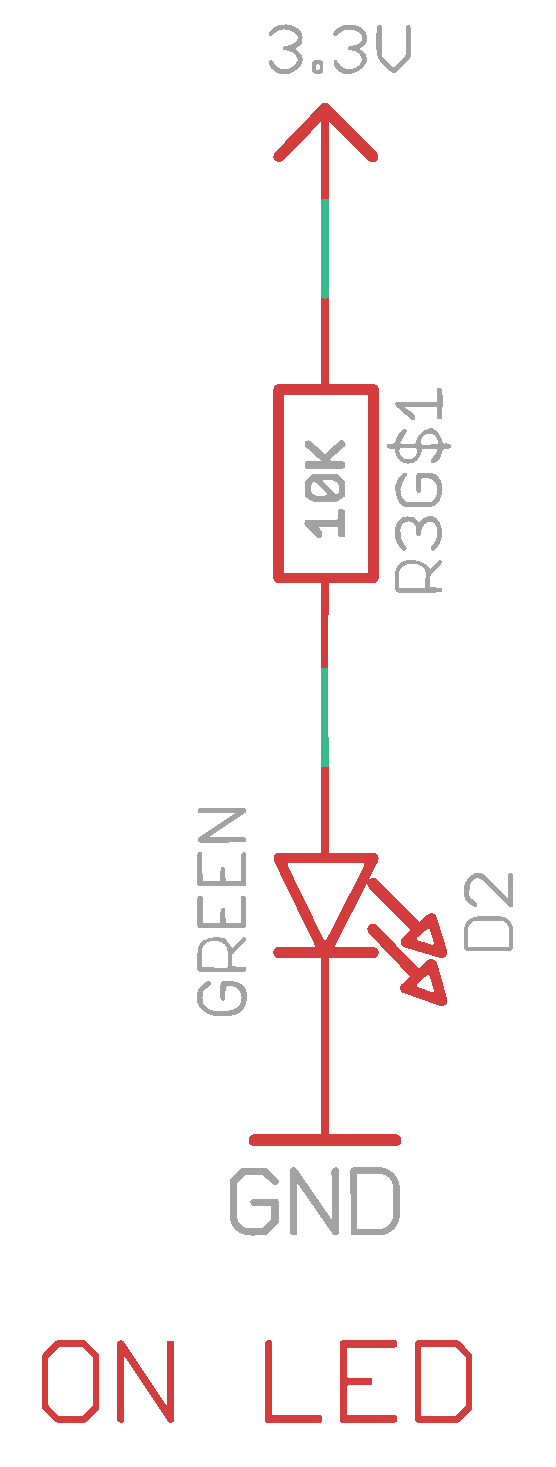
\includegraphics[width=0.16\linewidth]{../figures/mesures/led-imu}
	\caption{LED de vie de la carte d'adafruit (2.2V).}
	\label{fig:led-imu}
	\source{Schéma de la \href{https://cdn-learn.adafruit.com/assets/assets/000/092/544/original/sensors_BNO055_STEMMA_sch.png?1593120280}{carte BNO055 d'adafruit }}
\end{figure}

Comme le montre la figure \ref{fig:led-imu}, une LED reste constamment allumée lors de la mise sous tension de la carte de l'\gls{imu}. Elle présente une différence de potentiel de $2.2V$ à ses bornes, entraînant une consommation constante de $0.11mA$. Bien que cette consommation soit faible, elle est inutile. Dans le cadre de ce prototype, la LED n'a pas été débrasée, mais un adhésif a été collé dessus afin de limiter la pollution lumineuse sur la LED d'état qui passe par un guide-lumière.

\noindent\textbf{Permettre de changer de mode plus facilement} Permettre à l'utilisateur de facilement basculer entre le mode "auto-enclenchement" et "enclenchement manuel" permettrait d'éviter des consommations inutiles.



\subsection{Bus de communications}
Avec le code implémenté dans le microcontrôleur, les différents périphériques fonctionnent correctement et la communication avec les différents bus est opérationnelle. C'est pourquoi, dans cette section, l'objectif principal est de mesurer la qualité et l'intégrité des signaux plutôt que d'analyser les différents protocoles.

\subsubsection{Communication I2C} \label{ssec:Comm-I2C}
La communication I2C s'effectue entre la centrale inertielle BNO055 et le microcontrôleur. Par ce bus, les configurations du registre de l'\gls{imu} ainsi que les données inertielles mesurées, en fonction de ces configurations, sont transmises. Comme nous avons pu le voir précédemment, cette communication est effective et les données sont cohérentes. Dans ce contexte, nous examinerons si l'intervalle entre les mesures est respecté, la durée de ces mesures, ainsi que la qualité des signaux I2C.


\paragraph{Méthode de mesure}
La boîte noire a été configurée pour transmettre et enregistrer des données inertielles à intervalles de 2 secondes. De plus, les mesures ont été prises pendant la transmission des données inertielles, et non lors de la configuration. Enfin, les trames ont été décodées automatiquement par l'oscilloscope grâce à sa fonction "Protocol".

\paragraph{Schéma de mesure} Le schéma de mesure est présenté sur la figure \ref{fig:schema-mesure-i2c}.


\begin{figure}[H]
	\centering
	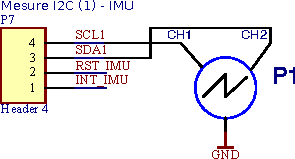
\includegraphics[width=0.4\linewidth]{../figures/mesures/I2C/Schema-mesure-i2c}
	\caption{Schéma de mesure, mesures I2C.}
	\label{fig:schema-mesure-i2c}
	\source{Auteur}
\end{figure}

\paragraph{Mesures}
Comme le montre la figure \ref{fig:intervale-2s}, il y a un délai de $1.98$ secondes entre l'envoi de deux sets de données de la centrale inertielle.


\begin{figure}[H]
	\centering
	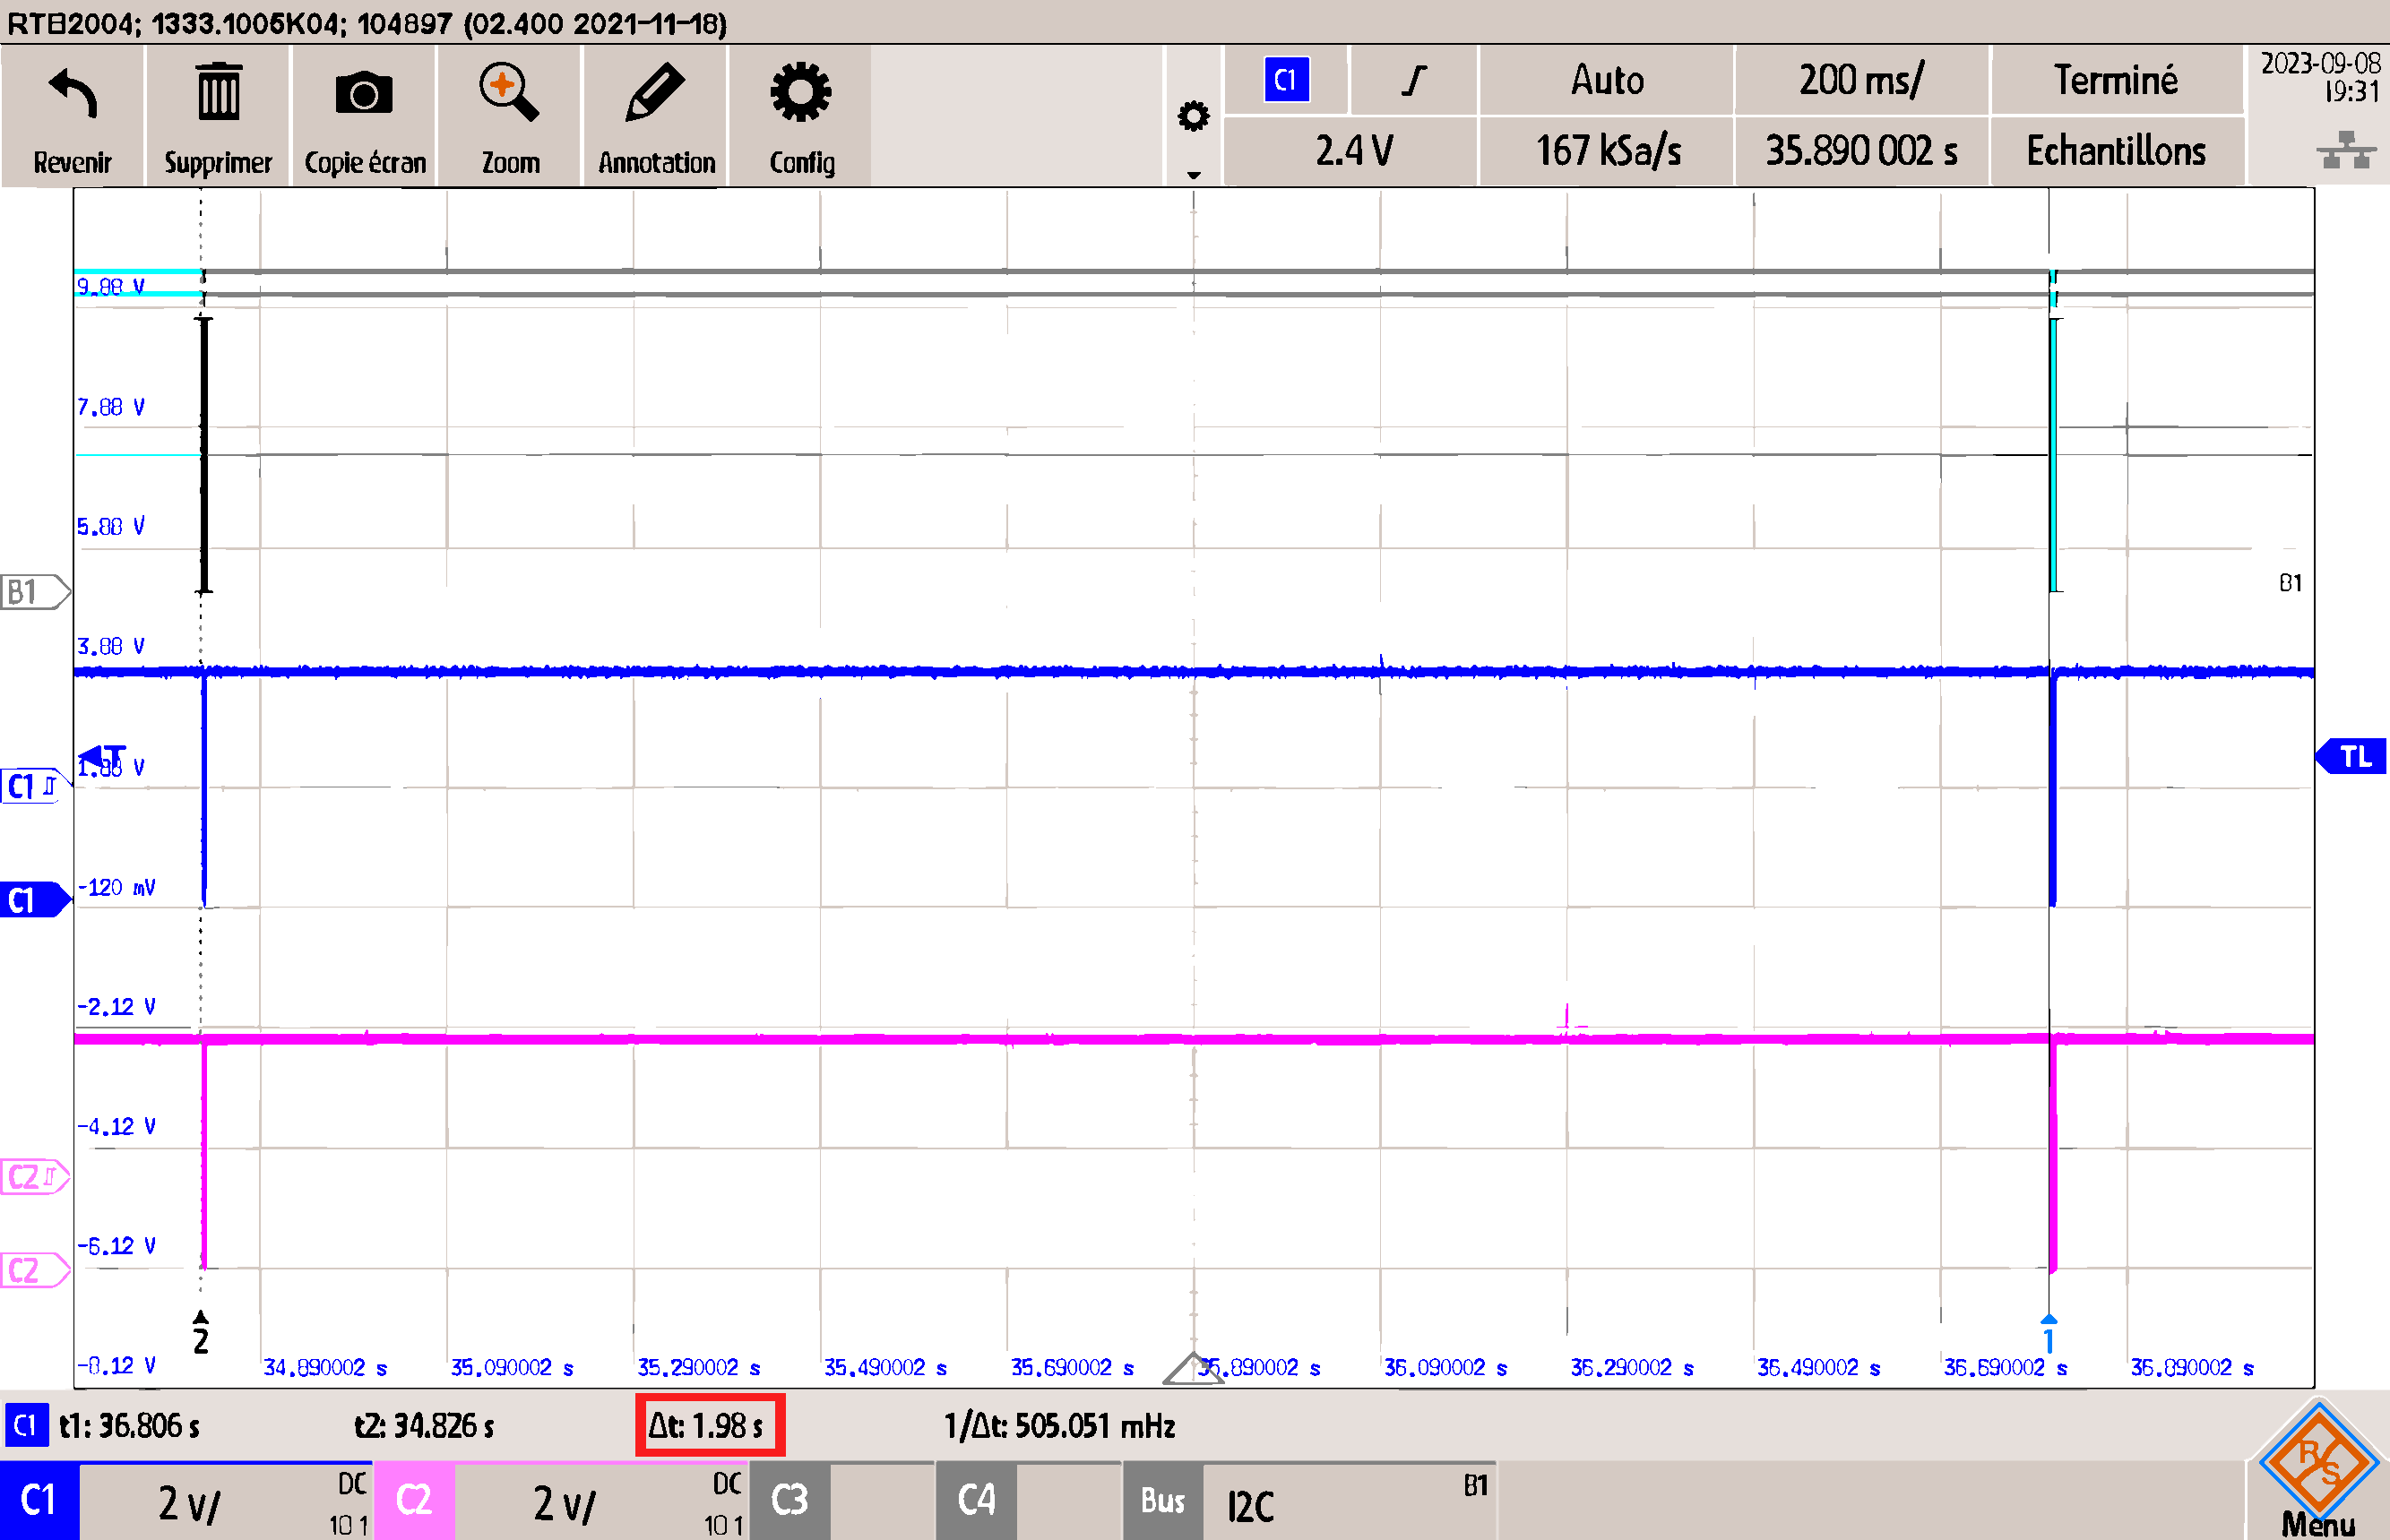
\includegraphics[width=.7\linewidth]{../figures/mesures/I2C/Intervale-2s}
	\caption{Intervale entre deux mesures, config. 2 secondes.}
	\label{fig:intervale-2s}
	\source{Auteur}
\end{figure}

Malgré la légère différence sur la figure \ref{fig:intervale-2s} de $20ms$, probablement due à une imprécision de mesure, nous pouvons conclure que l'intervalle entre les mesures respecte bien la configuration établie, même après modifications de celle-ci.

Sur la figure \ref{fig:duree-comm}, nous observons la durée d'une trame de mesures qui englobe toutes les données mentionnées dans la section \ref{sssec:IMU-data}. La durée de transmission d'un set de mesure est de $2.274ms$. Compte tenu que le bus est configuré en mode "fast" à $400 kbit/s$, cela suggère qu'environ $\sim910$ bits ont été transmis, ce qui explique la densité des données rendant la figure peu lisible.

\begin{figure}[H]
	\centering
	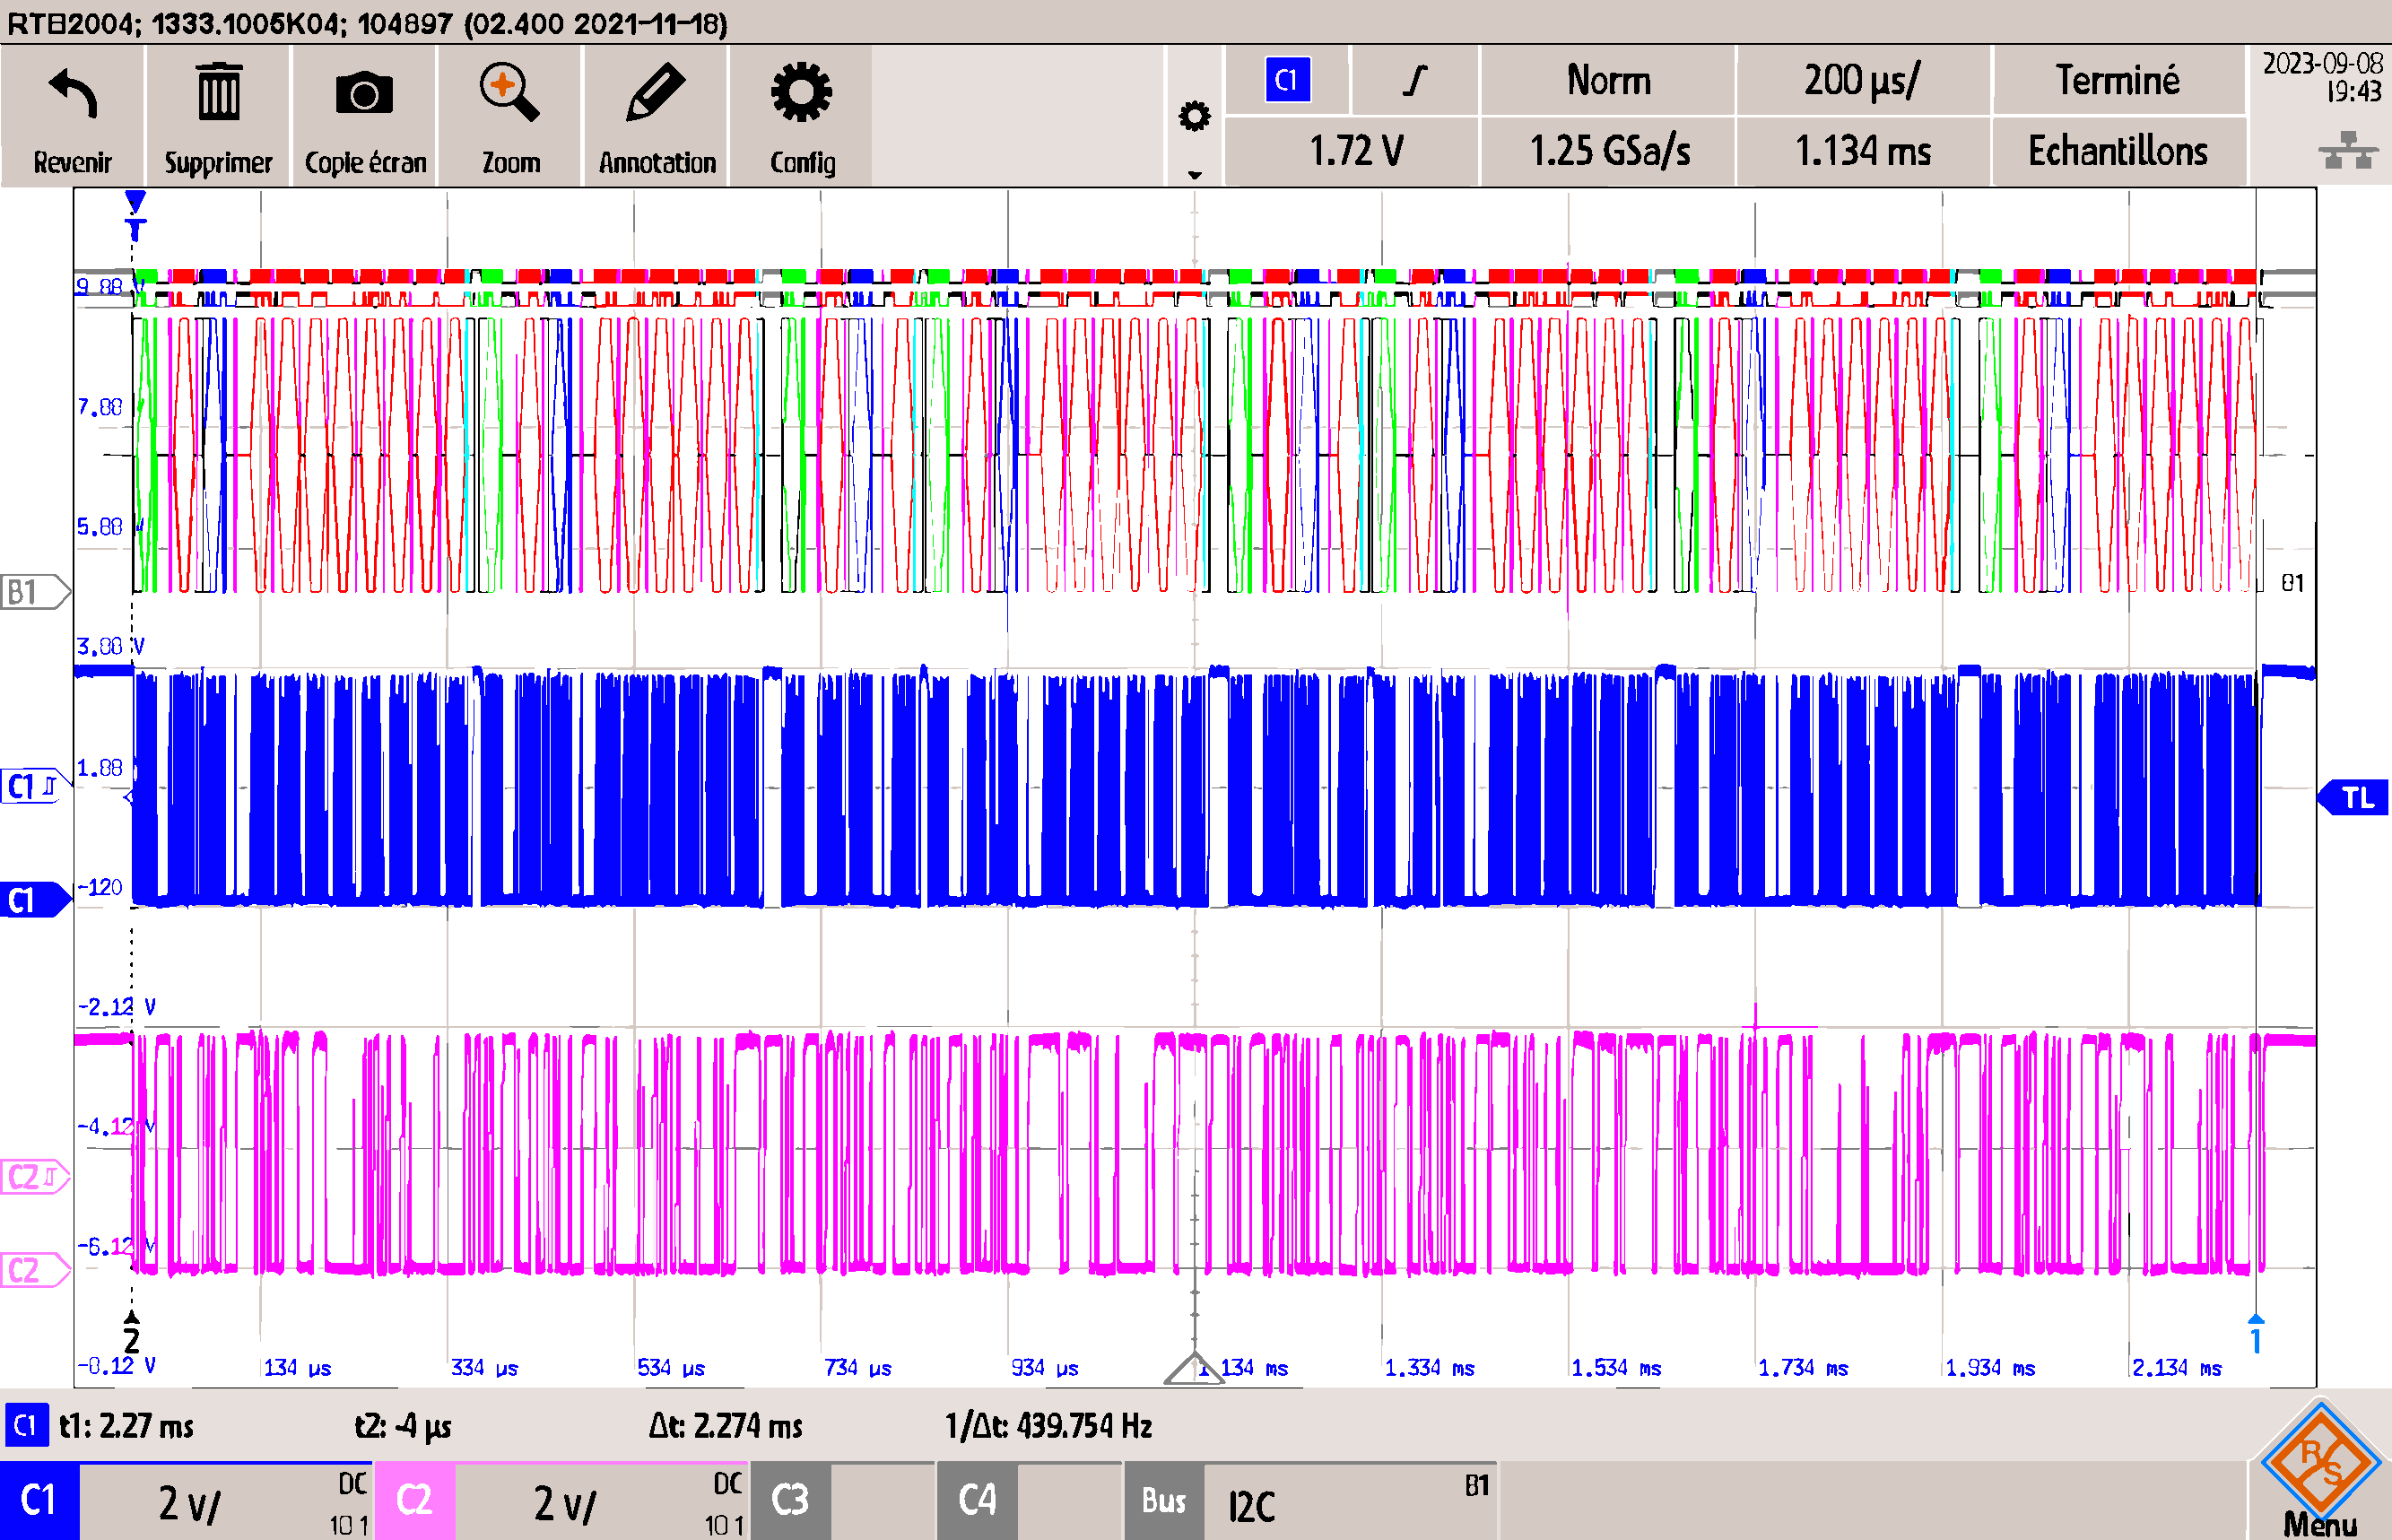
\includegraphics[width=.7\linewidth]{../figures/mesures/I2C/duree-comm}
	\caption{Durée d'une mesure.}
	\label{fig:duree-comm}
	\source{Auteur}
\end{figure}

Sur la figure \ref{fig:tramme-mesure}, nous observons le début d'une communication avec l'\gls{imu}. Le premier byte (\textbf{0x28}) correspond à l'adresse du BNO055. Ensuite, le registre \textbf{0x28} est adressé : il s'agit du registre contenant les données \textbf{LSB} de l'accélération linéaire. Les flancs des bits transmis semblent suffisamment nettes et peu parasités pour une bonne communication.

\begin{figure}[H]
	\centering
	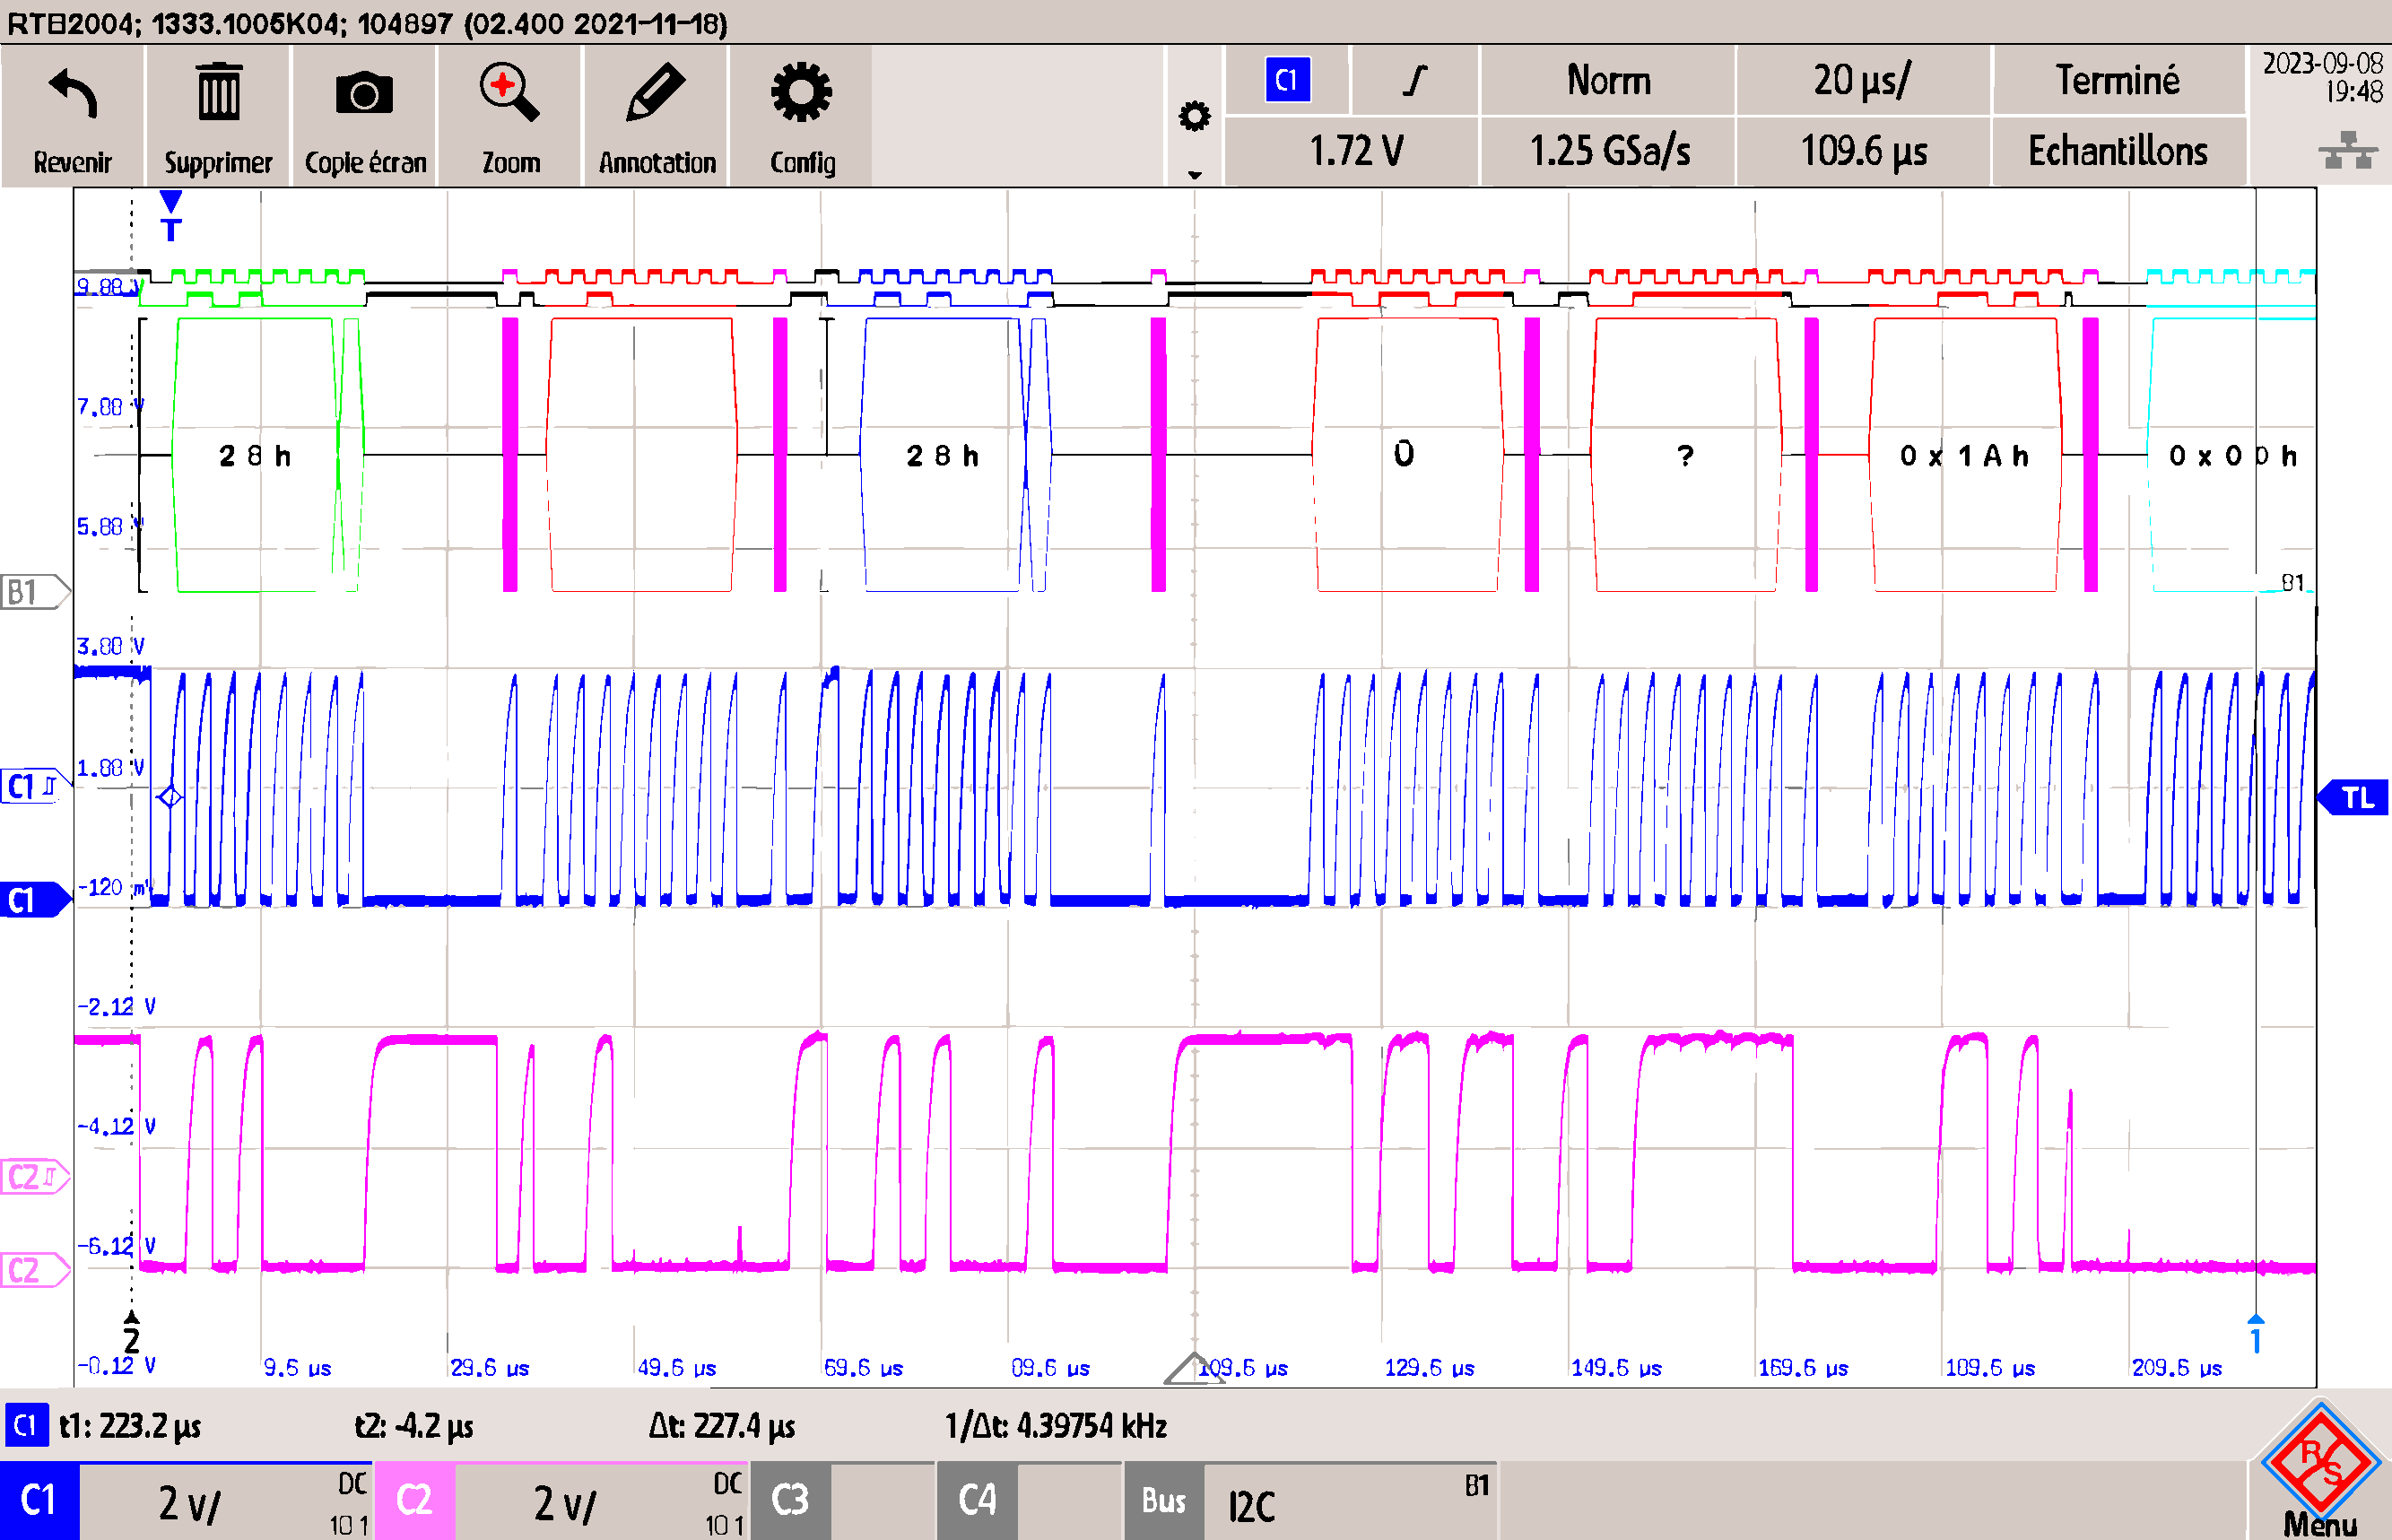
\includegraphics[width=.7\linewidth]{../figures/mesures/I2C/Tramme-mesure}
	\caption{Début de tramme d'une mesure.}
	\label{fig:tramme-mesure}
	\source{Auteur}
\end{figure}

\clearpage

\subsubsection{Communication UART GNSS} \label{ssec:Comm-UART}
Dans cette section, nous analyserons les différentes caractéristiques de la communication UART entre le microcontrôleur et le module \gls{gnss}.

\paragraph{Méthode de mesure} Pour réaliser ces mesures, le système a été activé et le \gls{gnss} a été configuré par défaut à une fréquence de \textbf{1Hz}.

\paragraph{Schéma de mesure} Le schéma de mesure est présenté sur la figure \ref{fig:scheam-mesure-uart-gnss}, nous nous intéressants ici, qu'au message envoyés par le GNSS dans sa configuration par défaut. 
\begin{figure}[h]
	\centering
	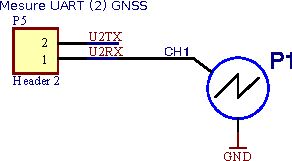
\includegraphics[width=0.4\linewidth]{../figures/mesures/UART/scheam-mesure-uart-gnss}
	\caption{Schéma de mesure \gls{gnss}.}
	\label{fig:scheam-mesure-uart-gnss}
	\source{Auteur}
\end{figure}



\paragraph{Mesures}
Sur la figure \ref{fig:interval-gnss}, nous observons l'intervalle entre les messages GNSS. Effectivement, cet intervalle est de $1s$, offrant ainsi suffisamment de temps au \gls{mcu} pour traiter ces données, que ce soit pour les afficher sur un terminal ou les enregistrer sur la carte SD.

\begin{figure}[H]
	\centering
	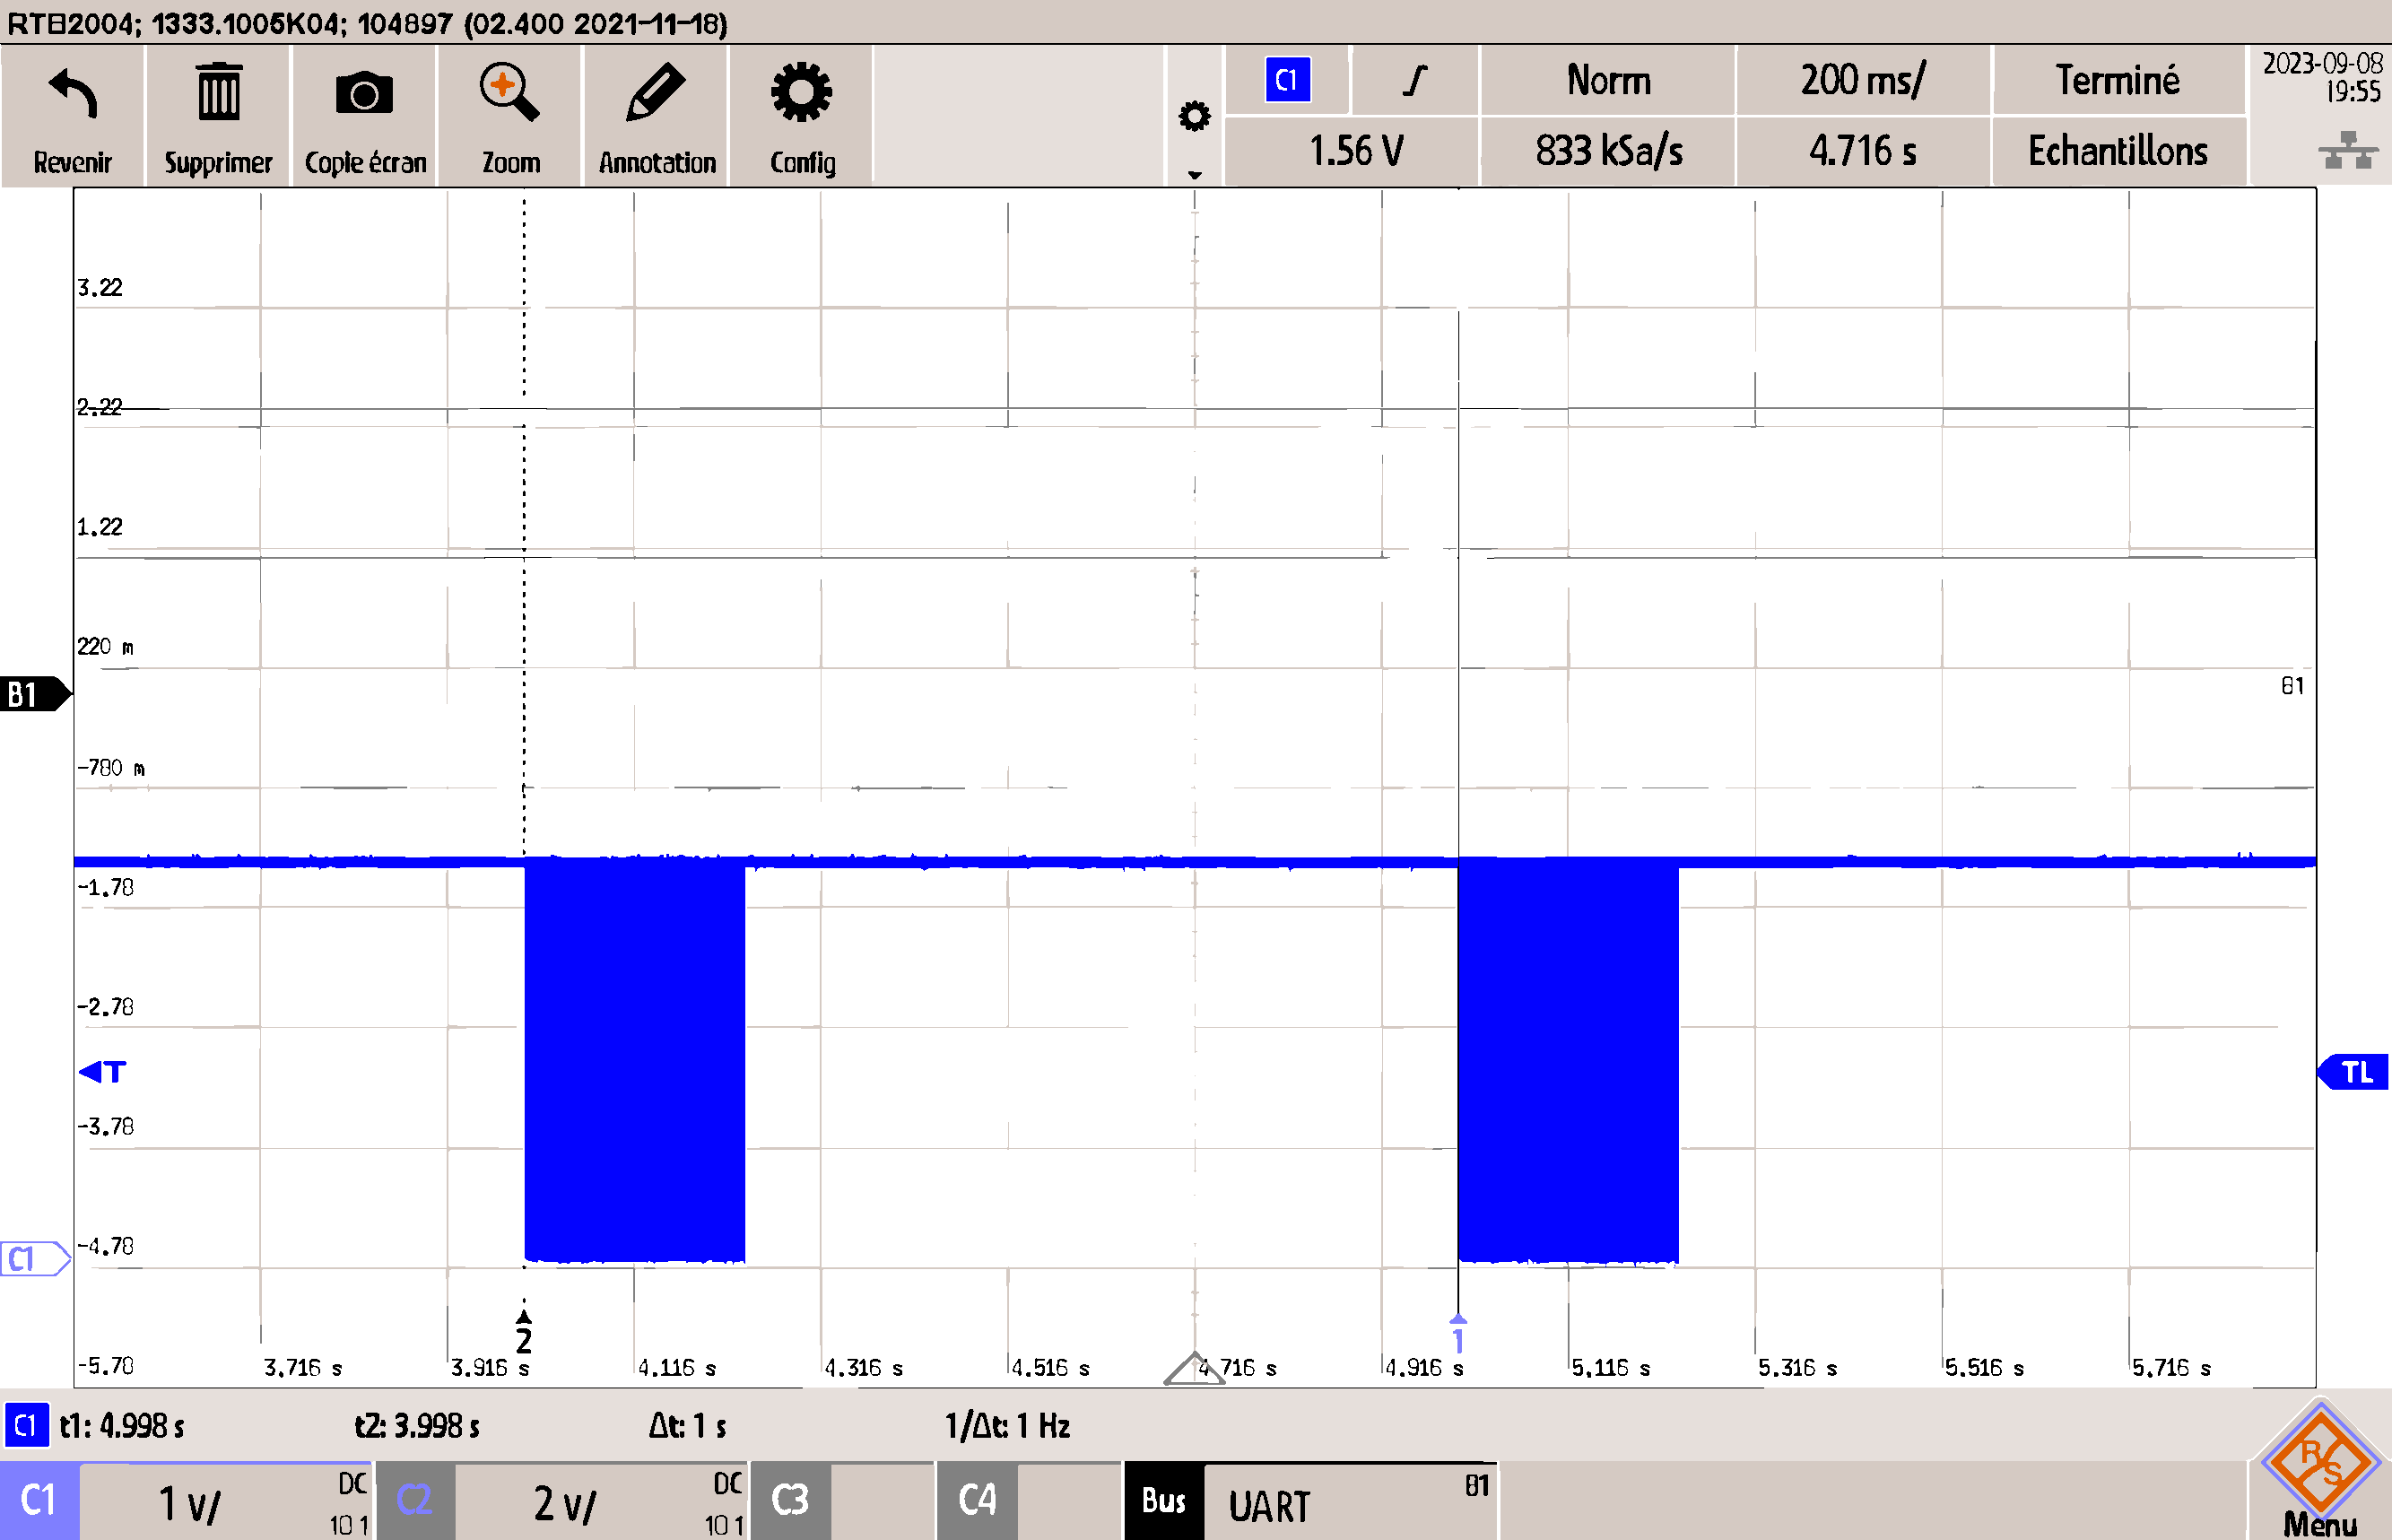
\includegraphics[width=0.7\linewidth]{../figures/mesures/UART/interval-gnss}
	\caption{Intervale entre les données NMEA.}
	\label{fig:interval-gnss}
	\source{Auteur}
\end{figure}

Sur la figure \ref{fig:duree-comm-gnss}, nous constatons que la durée d'envoi des messages \textbf{NMEA} est de $234.4 ms$. Sachant que l'intervalle entre les transmissions est de $1s$, cela laisse une fenêtre de $756ms$ au \gls{mcu} pour traiter ces données. Cette période est largement suffisante pour la transmission des données via le second UART (opérant au même baud rate) ou vers la carte SD, dont la fréquence est nettement supérieure ($10MHz$). Si nous considérons la durée des transmissions de l'\gls{imu}, qui est de $2.274ms$, nous estimons avec une marge qu'environ $\sim400ms$ des $756ms$ disponibles sont utilisés pour traiter les données. Ce temps de traitement pourrait être encore diminuée si la fréquence d'enregistrement du \gls{gnss} était baissée. Ainsi, nous pourrions envisager d'obtenir jusqu'à $\sim155$ mesures d'\gls{imu} dans l'intervalle donné.


\begin{figure}[H]
	\centering
	\includegraphics[width=0.7\linewidth]{../figures/mesures/UART/duree-comm-gnss}
	\caption{Durée d'une communication avec le GNSS.}
	\label{fig:duree-comm-gnss}
	\source{Auteur}
\end{figure}

La figure \ref{fig:message-nmea-rmc} illustre le décodage d'une trame \textbf{NMEA} correspondant à un message \textbf{RMC}. Les données de ce message sont similaires à celles présentées dans la section \ref{sssec:GNSS-data}. Les signaux présentent une bonne intégrité et sont correctement interprétés par le microcontrôleur. Ils sont ensuite retransmis à la carte SD et au second UART avec justesse.


\begin{figure}[H]
	\centering
	\includegraphics[width=0.7\linewidth]{../figures/mesures/UART/message-NMEA-RMC}
	\caption{Message RMC du protocole NMEA.}
	\label{fig:message-nmea-rmc}
	\source{Auteur}
\end{figure}

Nous observons sur la figure \ref{fig:message-nmea-rmc} le message décodé par l'oscilloscope \hyperref[ssec:Liste-materiel]{\textbf{P1}} : \textbf{\$GN\textcolor{blue}{RMC},,\textcolor{red}{V},,,,,,,,,N*}

\clearpage

\subsubsection{Communication SPI, carte SD} \label{ssec:Comm-SPI}
\paragraph{Méthode de mesure}
\paragraph{Schéma de mesure} Le schéma de mesure est présenté sur la figure
\paragraph{Mesures}

\begin{figure}[H]
	\centering
	\includegraphics[width=0.7\linewidth]{../figures/mesures/SPI/freq-spi}
	\caption{Mesure fréquence clock SPI.}
	\label{fig:freq-spi}
	\source{Auteur}
\end{figure}

\begin{figure}[H]
	\centering
	\includegraphics[width=0.7\linewidth]{../figures/mesures/SPI/densite-comm}
	\caption{Densité de la communication SPI.}
	\label{fig:densite-comm}
	\source{Auteur}
\end{figure}



\section{Caractéristiques du produit fini} \label{sec:Carac-finis}

% ---- Bibliographie ----
%\input{bibliography}

\clearpage

\section{Conclusion}



\newpage
\nocite{*}
\section{Bibliographie}
\bibliography{Biblio_TDD} 
\bibliographystyle{ieeetr}


% ANNEXES
\clearpage
\section{Annexes}

\end{document}
